\documentclass{beamer}

\input{preamble.tex}
\usepackage{breqn} % Breaks lines

\usepackage{amsmath}
\usepackage{mathtools}

\usepackage{pdfpages} % \includepdf

\usepackage{listings} % R code
\usepackage{verbatim} % verbatim

% Video stuff
\usepackage{media9}

% packages for bibs and cites
\usepackage{natbib}
\usepackage{har2nat}
\newcommand{\possessivecite}[1]{\citeauthor{#1}'s \citeyearpar{#1}}
\usepackage{breakcites}
\usepackage{alltt}

% Setup math operators
\DeclareMathOperator{\E}{E} \DeclareMathOperator{\tr}{tr} \DeclareMathOperator{\se}{se} \DeclareMathOperator{\I}{I} \DeclareMathOperator{\sign}{sign} \DeclareMathOperator{\supp}{supp} \DeclareMathOperator{\plim}{plim}
\DeclareMathOperator*{\dlim}{\mathnormal{d}\mkern2mu-lim}
\newcommand\independent{\protect\mathpalette{\protect\independenT}{\perp}}
   \def\independenT#1#2{\mathrel{\rlap{$#1#2$}\mkern2mu{#1#2}}}
\newcommand*\colvec[1]{\begin{pmatrix}#1\end{pmatrix}}

\newcommand{\myurlshort}[2]{\href{#1}{\textcolor{gray}{\textsf{#2}}}}


\begin{document}

\imageframe{./lecture_includes/mixtape_did_cover.png}


% ---- Content ----

\section{Background material}
\subsection{Introduction}

\begin{frame}{Introduction}

\begin{itemize}

\item Scott Cunningham, Ben H. Williams Professor, Baylor Economics Dept
\item Research interests: mental illness and corrections, sex work, abortion policy, drug policy
\item Author of \underline{Causal Inference: the Mixtape} (Yale Press 2021)
\item Today we will review new material in diff-in-diff and review code implementation and applications
\item All this is on github repo plus exercises

\end{itemize}

\end{frame}



\begin{frame}{Why diff-in-diff and differential timing?}

\begin{itemize}
\item We will be discussing some of the newer material on difference-in-differences with differential timing
\item Fairly rapid advances over last six years in methodologies
\item Arguably the most recent wave of updates to our understanding of a technique that we thought was probably pretty straightforward
\item Difference-in-differences is as we'll see very straightforward, but \emph{regression} is less straightforward
\end{itemize}

\end{frame}

\begin{frame}{Differential timing outline}

We will cover some of the properties of twoway fixed effects (TWFE), some solutions and my personal opinions

\bigskip

\begin{enumerate}
	\item Brief review of DiD history, potential outcomes and the ATT
	\item Difference-in-differences equation (``four averages and three differences'') and the parallel trends assumption
	\item TWFE Pathologies in static specification
		\begin{itemize}
		\item Goodman-Bacon decomposition as diagnosis of the problem
		\item Callaway and Sant'Anna estimator as a cure
		\end{itemize}
	\item TWFE Pathologies in event study specification
		\begin{itemize}
		\item Sun and Abraham as both a diagnosis and a cure 
		\end{itemize}
	\item Application, practical advice and code
\end{enumerate}

\end{frame}	

\subsection{Three waves of Difference-in-Differences}

\begin{frame}{Diff-in-diff had belonged to the empiricists}

	\begin{figure}
	\caption{Currie, et al. (2020)}
	\includegraphics[scale=0.25]{./lecture_includes/currie_did.png}
	\end{figure}

\bigskip

\footnotesize

With some exception (e.g., Heckman, Ichimura and Todd 1997; Abadie 2005; Bertrand, Duflo and Mullainthan 2004), econometricians had not given it much notice

\end{frame}

\begin{frame}{First Wave of Diff-in-Diff}

\begin{itemize}
\item Difference-in-differences has evolved in three waves from 1983 to present in economics
\item First wave lasts from 1983 to 2011; second wave from 2011 to 2018; third wave from 2018 to present
\item Initially, the pick up was slow, mostly used by labor economists throughout the 1990s in the ``program evaluation'' area
\item No potential outcomes notation, no mention of parallel trends, no event studies -- only Ashenfelter's Dip, evidence of time varying selection bias

\end{itemize}

\end{frame}


\begin{frame}{Ashenfelter and Card coin the phrase difference-in-differences}

	\begin{figure}
	\caption{Ashenfelter and Card (1983)}
	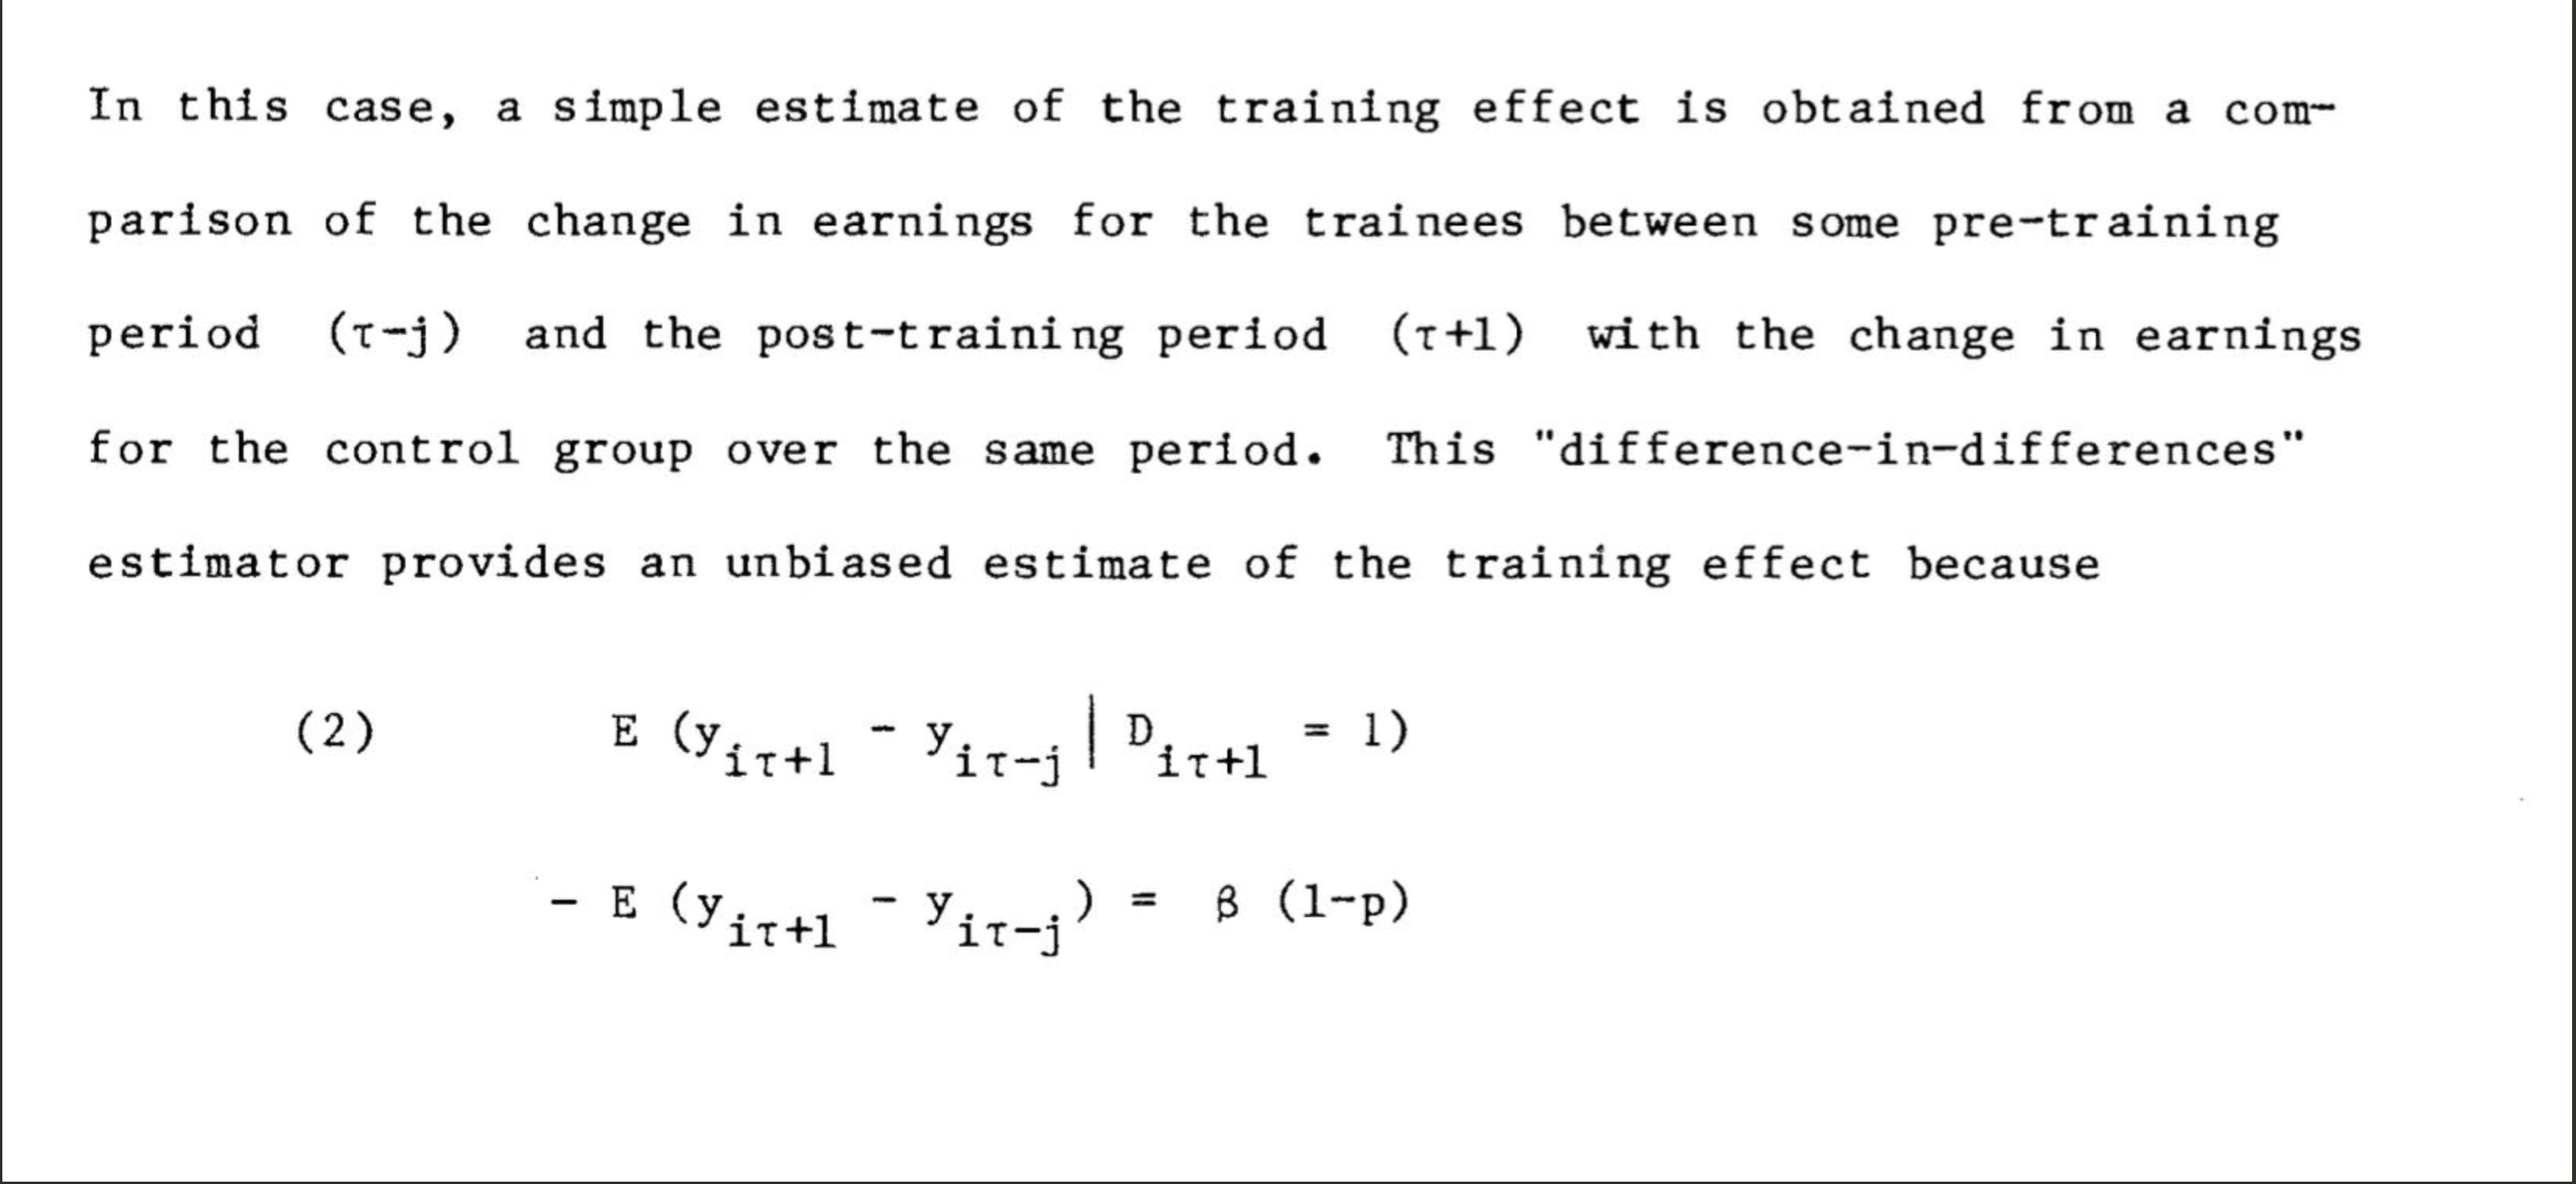
\includegraphics[scale=0.2]{./lecture_includes/orley1983.png}
	\end{figure}


\end{frame}




\begin{frame}{Card on Dips and Parallel Trends}

\begin{quote}
Scott: “This diff-in-diff thing. … I had the impression from stuff you’d written with Orley that you were a little lukewarm about the method a little bit. That it wasn’t always something that you’d found credible. Is that accurate?”

Dave: “Well in the original [job training program evaluation] case, you didn’t have parallel trends. … [Diff-in-diff] wasn’t something you could just count on to use out of the box.”

Scott: “So you were thinking about parallel trends from the very start?”

Dave: “Oh no, it’s right there in that 1985 paper with Orley that introduces the term difference-in-differences. Unfortunately we didn’t have a graph. When I teach the paper now I show the graph. It has a very large dip for the treatment group. And that’s the thing everyone nowadays calls the Ashenfelter Dip.” (my emphasis)


\end{quote}

\end{frame}


\begin{frame}{But parallel trends does not yet appear}

	\begin{figure}
	\caption{No mention of parallel trends in Ashenfelter and Card (1985)}
	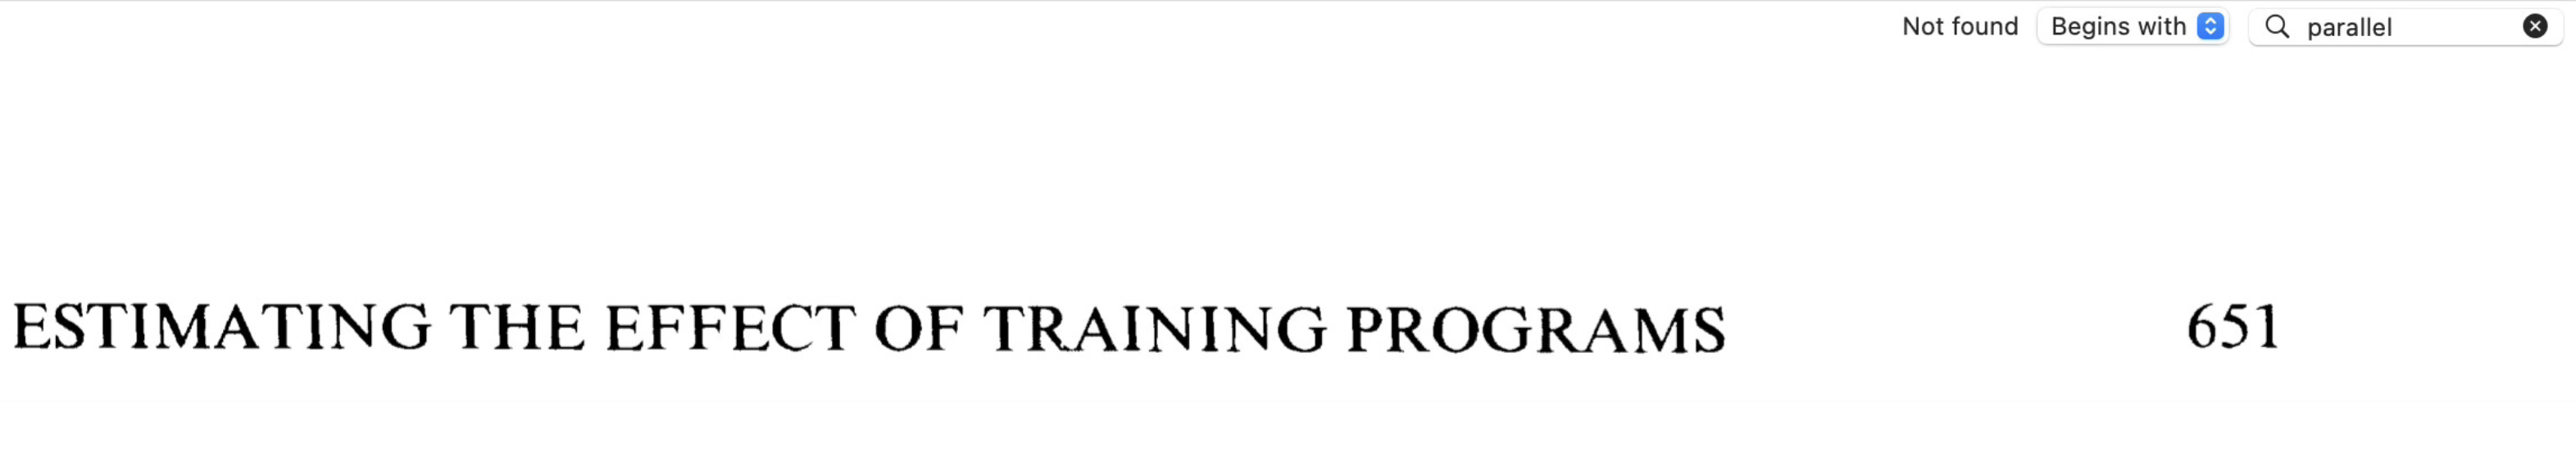
\includegraphics[scale=0.2]{./lecture_includes/nomention.png}
	\end{figure}

\end{frame}




\begin{frame}{Second wave grows faster than first}

\begin{itemize}
\item From 2011 to 2018, the share of NBER working papers that used diff-in-diff went from 11-12\% to 23\% in 2018, a little over 11 percentage points in only 7 years. 
\item It had taken 24 years to reach 11\% the first time, but only 7 years the second time. 
\item The second wave had a very fast growth rate. 
\item The second wave’s energy was stronger than the first.
\end{itemize}

\end{frame}

\begin{frame}{Second wave of DiD: event study and parallel trends}

	\begin{figure}
	\caption{Currie, et al. (2020)}
	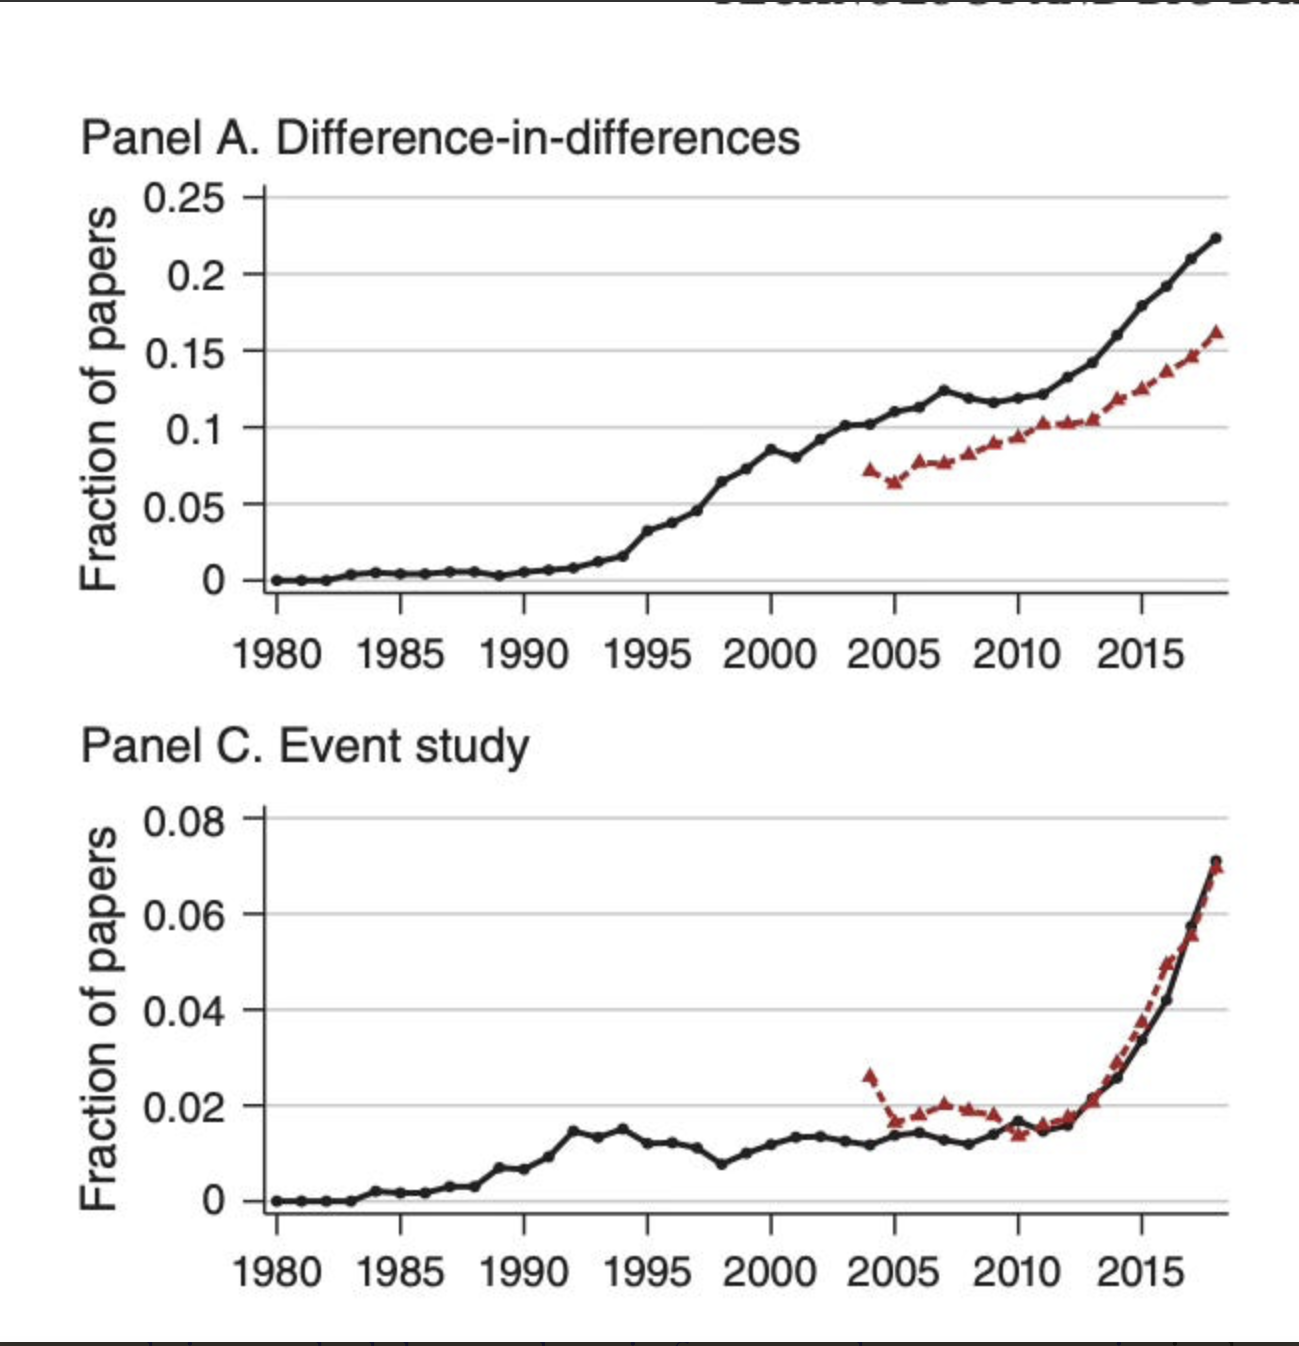
\includegraphics[scale=0.25]{./lecture_includes/secondwave.png}
	\end{figure}


\end{frame}

\begin{frame}{Second wave incorporates parallel trends and event studies}

\begin{itemize}

\item Prior to 2011, parallel trends was not a phrase used in combination with diff-in-diff
\item Event studies were used in finance to study abnormal stock market returns, not difference-in-differences
\item From 2011 to 2018, the share of NBER working papers that used diff-in-diff went from 11-12\% to 23\% and event study grows from 2\% to 7\%. 
\item It's more than just correlation -- papers that say  both``event study'' and ``parallel trends'' suddenly start appearing early to mid teens with exponential growth of 66\% a year
\end{itemize}

\end{frame}

\begin{frame}{Event study and parallel trends}

	\begin{figure}
	\caption{Exponential growth in both event study and parallel trends}
	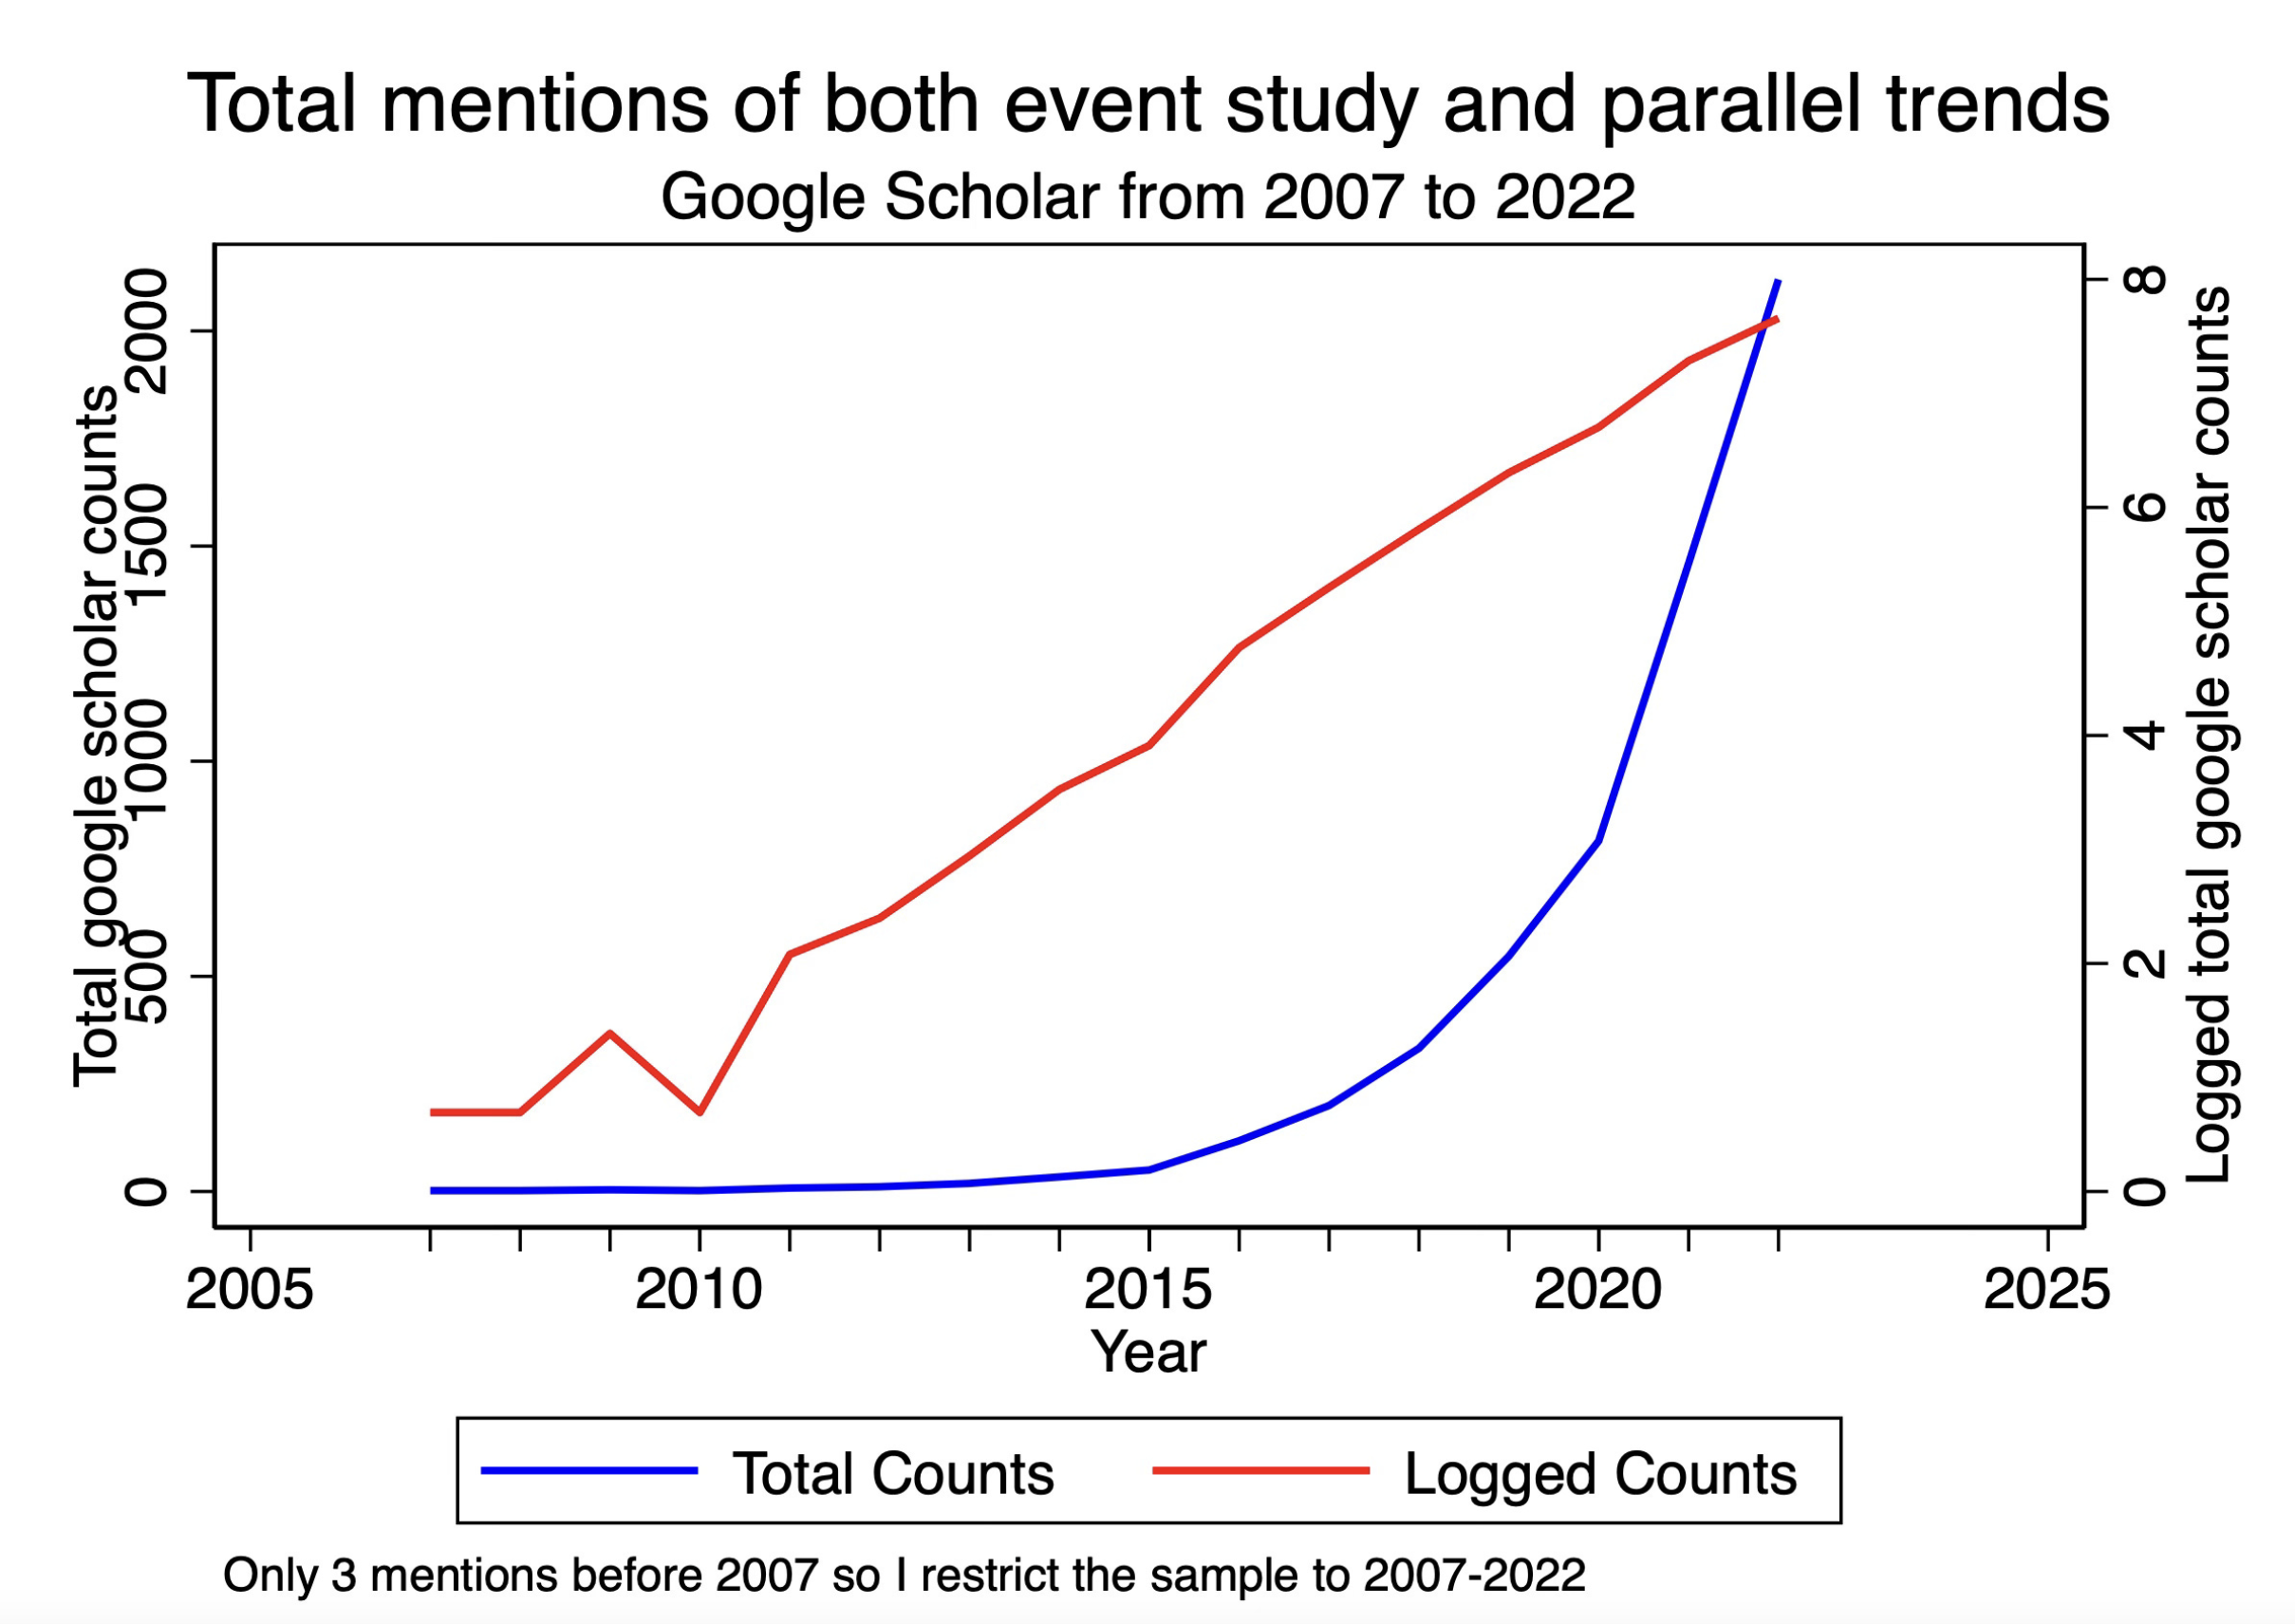
\includegraphics[scale=0.2]{./lecture_includes/event_pt.png}
	\end{figure}

\end{frame}


\begin{frame}{Second wave captures event studies}

\begin{itemize}
\item Second wave DiD brings in parallel trends and event studies to DiD designs, perhaps riding on the long tradition of Ashenfelter's Dip
\item But the explicit notation and identifying assumption is worked out gradually by different authors before being broadly adopted by practitioners 
\item Plotting of the words "parallel trends", "event study" and "common trends" in combination with papers with phrase "difference-in-differences"

\end{itemize}

\end{frame}


\begin{frame}{Incorporating PT and event study into diff-in-diff}

	\begin{figure}
	\caption{Growth in both event study and parallel trends}
	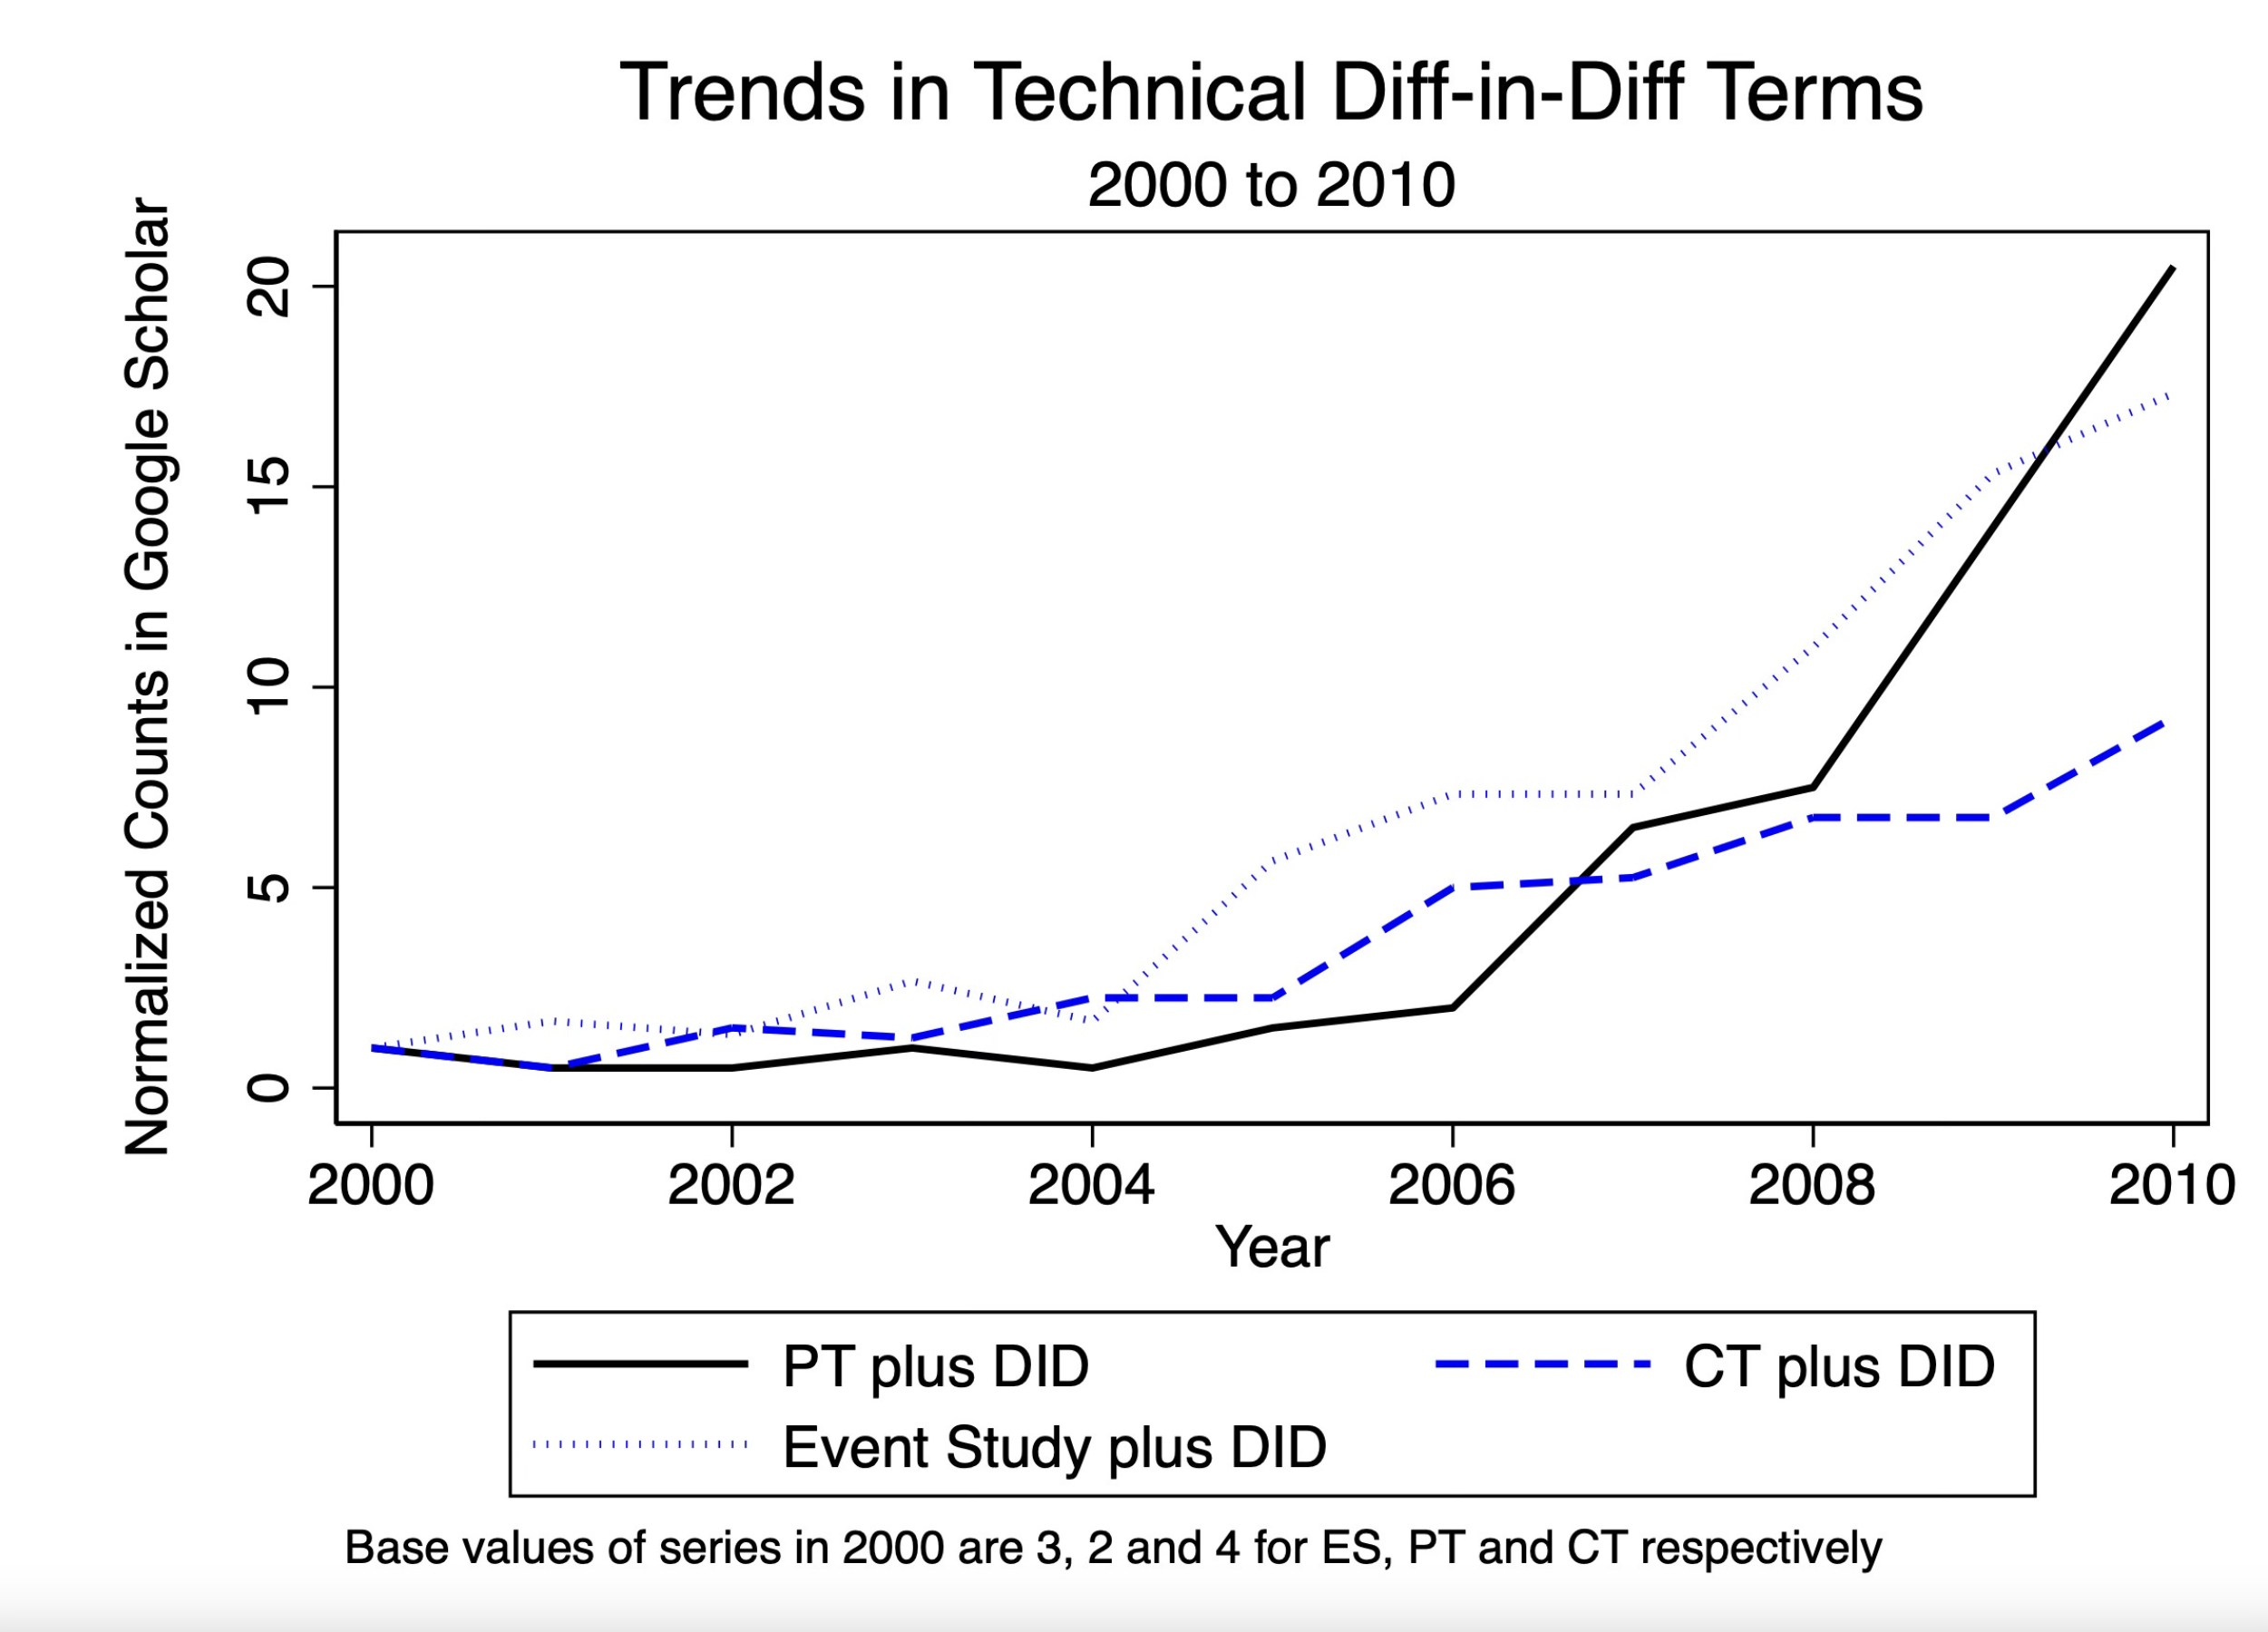
\includegraphics[scale=0.2]{./lecture_includes/espt_2}
	\end{figure}


\end{frame}

\begin{frame}{Incorporating PT and event study into diff-in-diff}

	\begin{figure}
	\caption{Growth in both event study and parallel trends}
	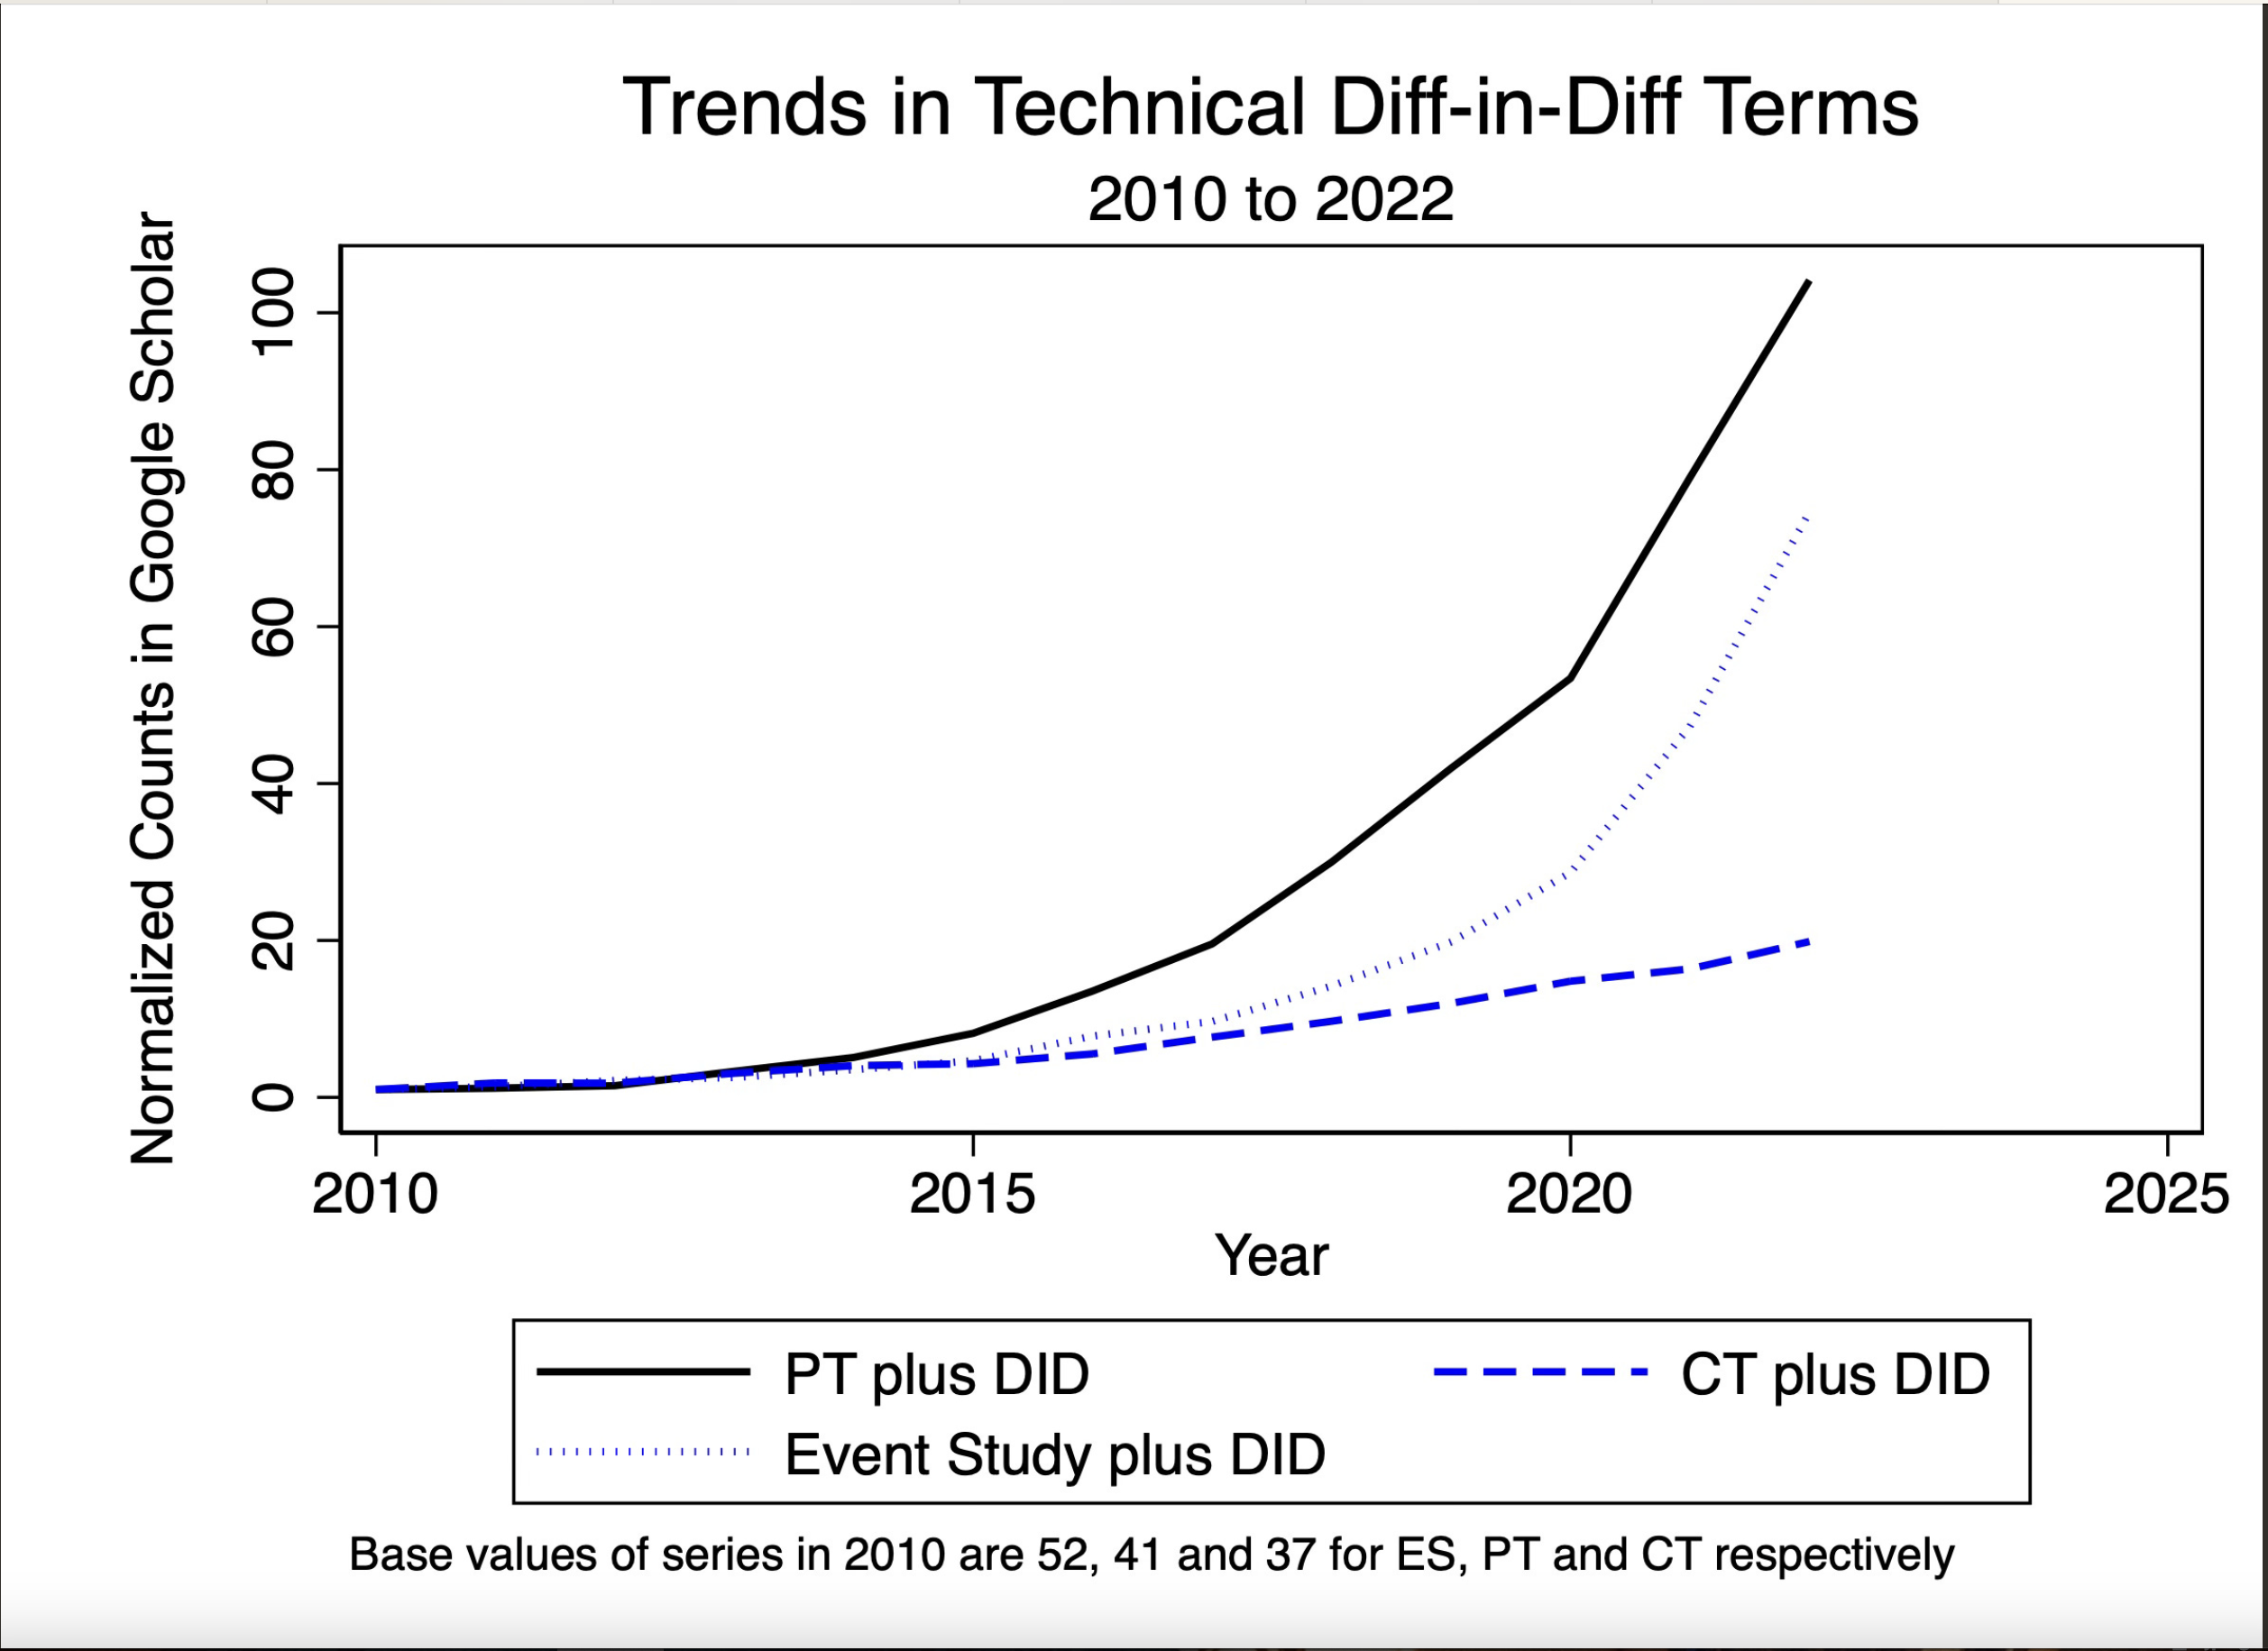
\includegraphics[scale=0.2]{./lecture_includes/espt_3}
	\end{figure}


\end{frame}





\begin{frame}{Parallel trends is introduced late}

\begin{itemize}

\item Early focus had tended to emphasize the year fixed effects, but authors did not typically mean ``parallel trends'' 
	\begin{quote}
	“Moreover, given the increasing dispersion of incomes and wages among all groups during that period, the common time effects (common trends) assumption among the unobservable components across the two groups may not be satisfied.” (Blundell and Dias 1999)
	\end{quote}
\item Early identification was an independent assumption by Blundell, but this was viewed as too strong by Athey and Imbens (2006)

\begin{quote}
“Note that the full independence assumption $\varepsilon_i \independent(G_i,T_i)$ (e.g., Blundell and MaCurdy (2000)) is stronger than necessary for [DiD] to give the average treatment effect.”
\end{quote}

\end{itemize}

\end{frame}


\begin{frame}{Heckman, et al. (1997) introduce potenial outcomes}


\begin{itemize}
\item First time we see parallel trends expressed (without name) using potential outcomes, though, is a conditional parallel trends assumption by Heckman, Ichimura and Todd (1997)

\bigskip

	\begin{figure}
	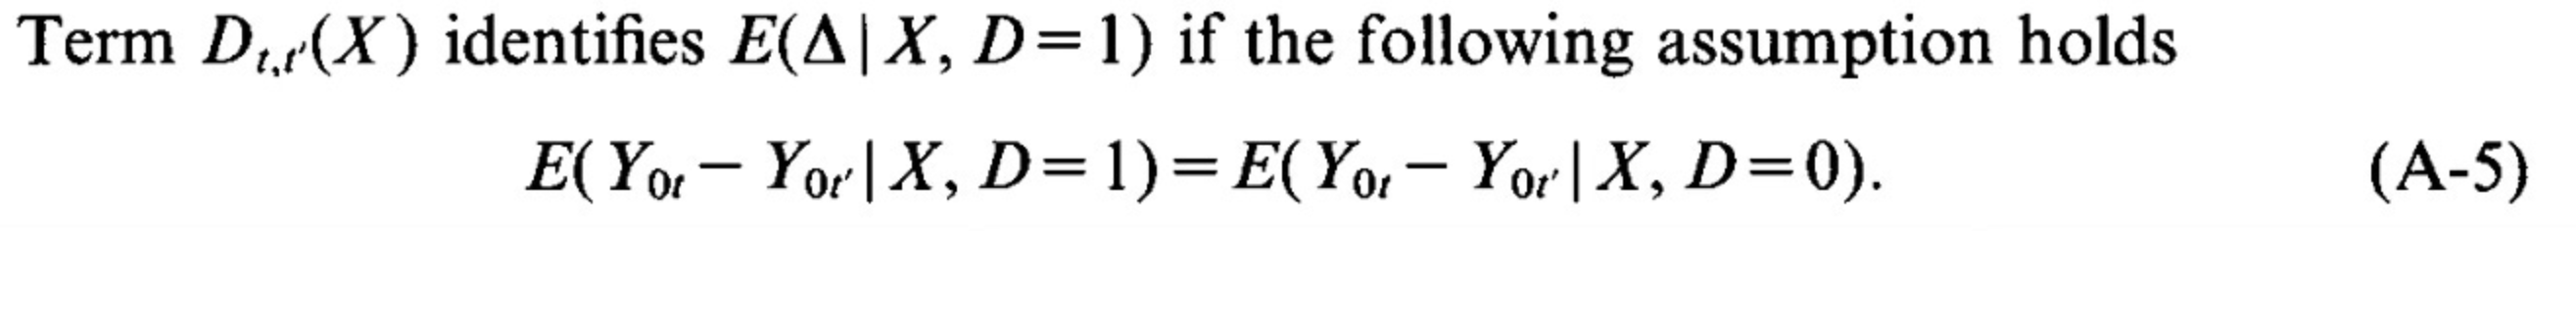
\includegraphics[scale=0.2]{./lecture_includes/heckman_cpt}
	\end{figure}


\item Angrist and Pischke (2009) chapter 5 is entitled "Parallel Worlds: Fixed Effects, Difference-in-Differences and Panel Data''
\item But phrase ``parallel trends'' does not appear (actually unclear when it starts getting used) -- but we do see this diagram
\end{itemize}


\end{frame}




\begin{frame}{Mostly Harmless and Parallel Trends}


	\begin{figure}
	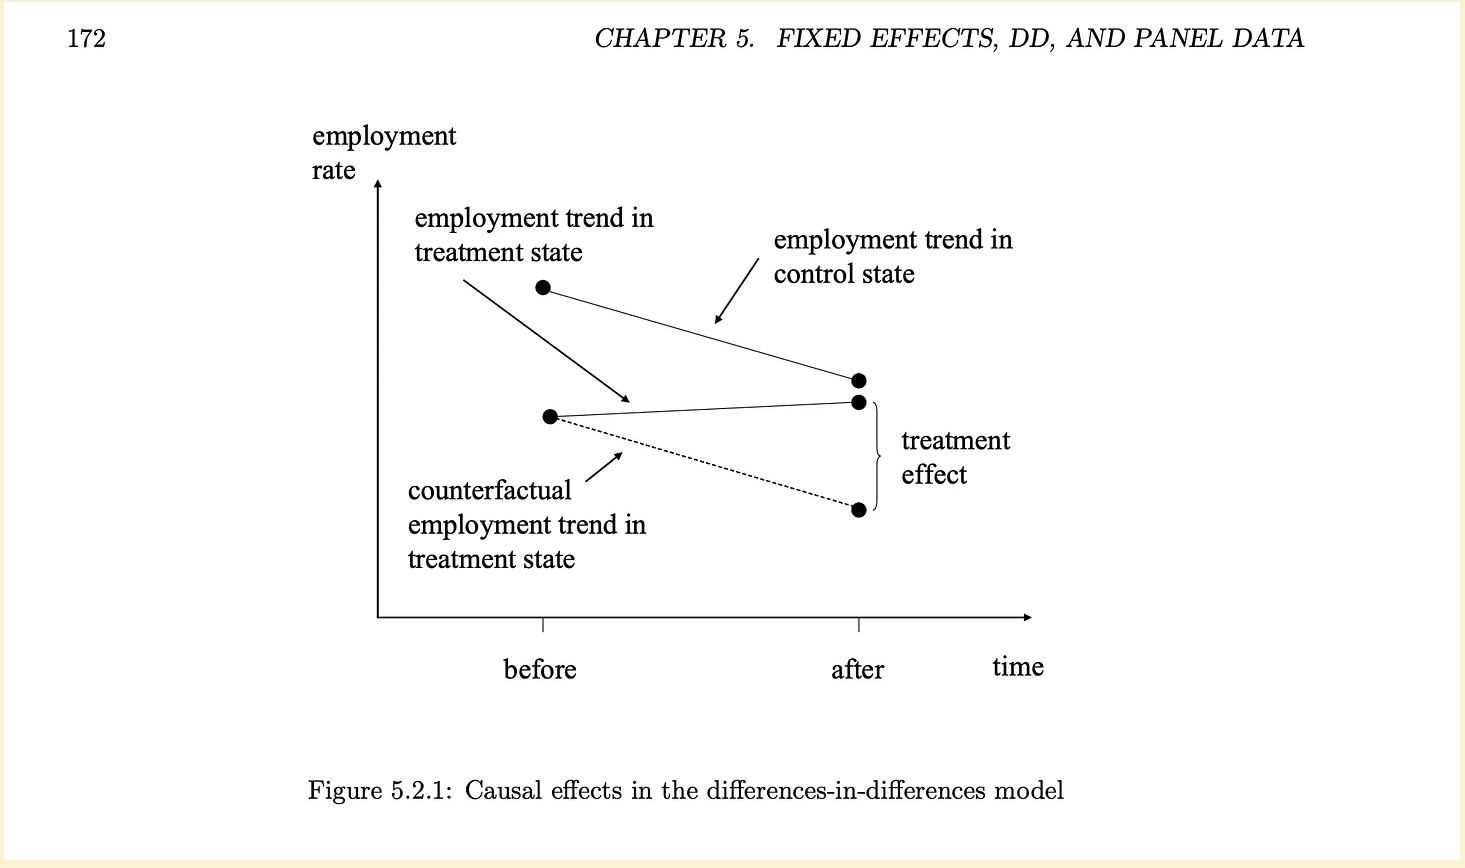
\includegraphics[scale=0.45]{./lecture_includes/mhe_pt}
	\end{figure}



\end{frame}








\begin{frame}{Introducing Event Studies to Diff-in-Diff}

	\begin{figure}
	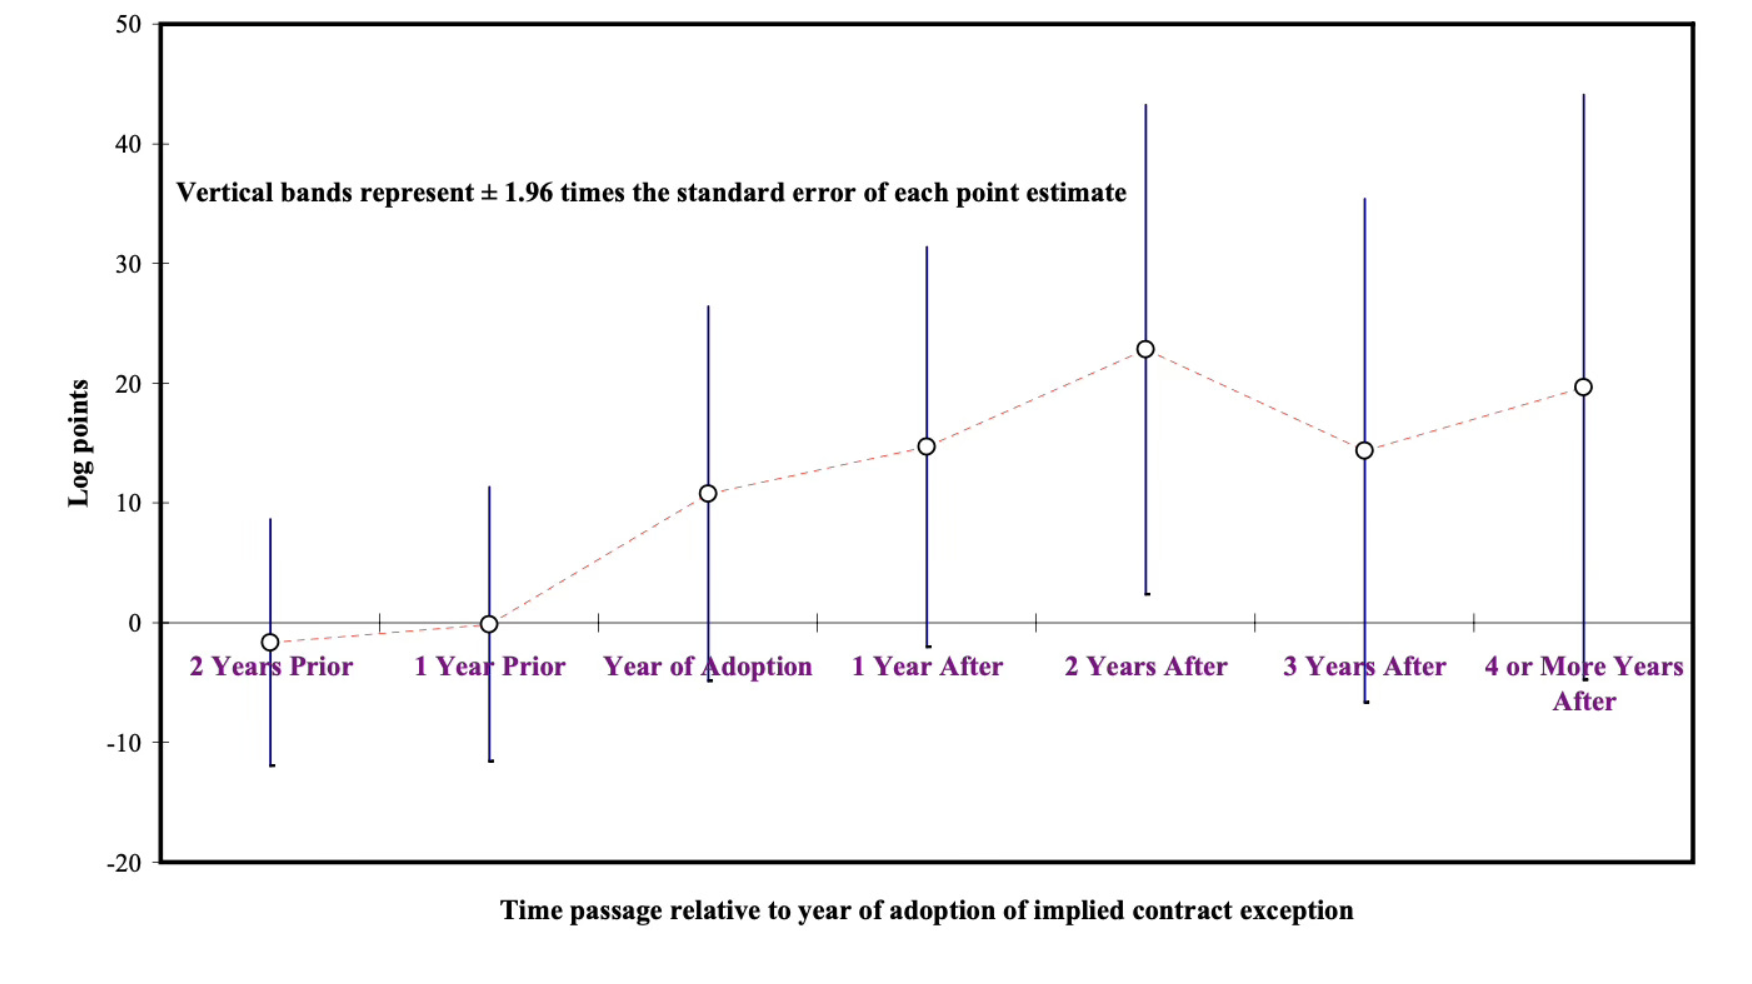
\includegraphics[scale=0.35]{./lecture_includes/autor2003}
	\caption{David Autor (2003) ``unjust dismissals'' paper}
	\end{figure}

\end{frame}

\begin{frame}{Constant effects model}

	\begin{figure}
	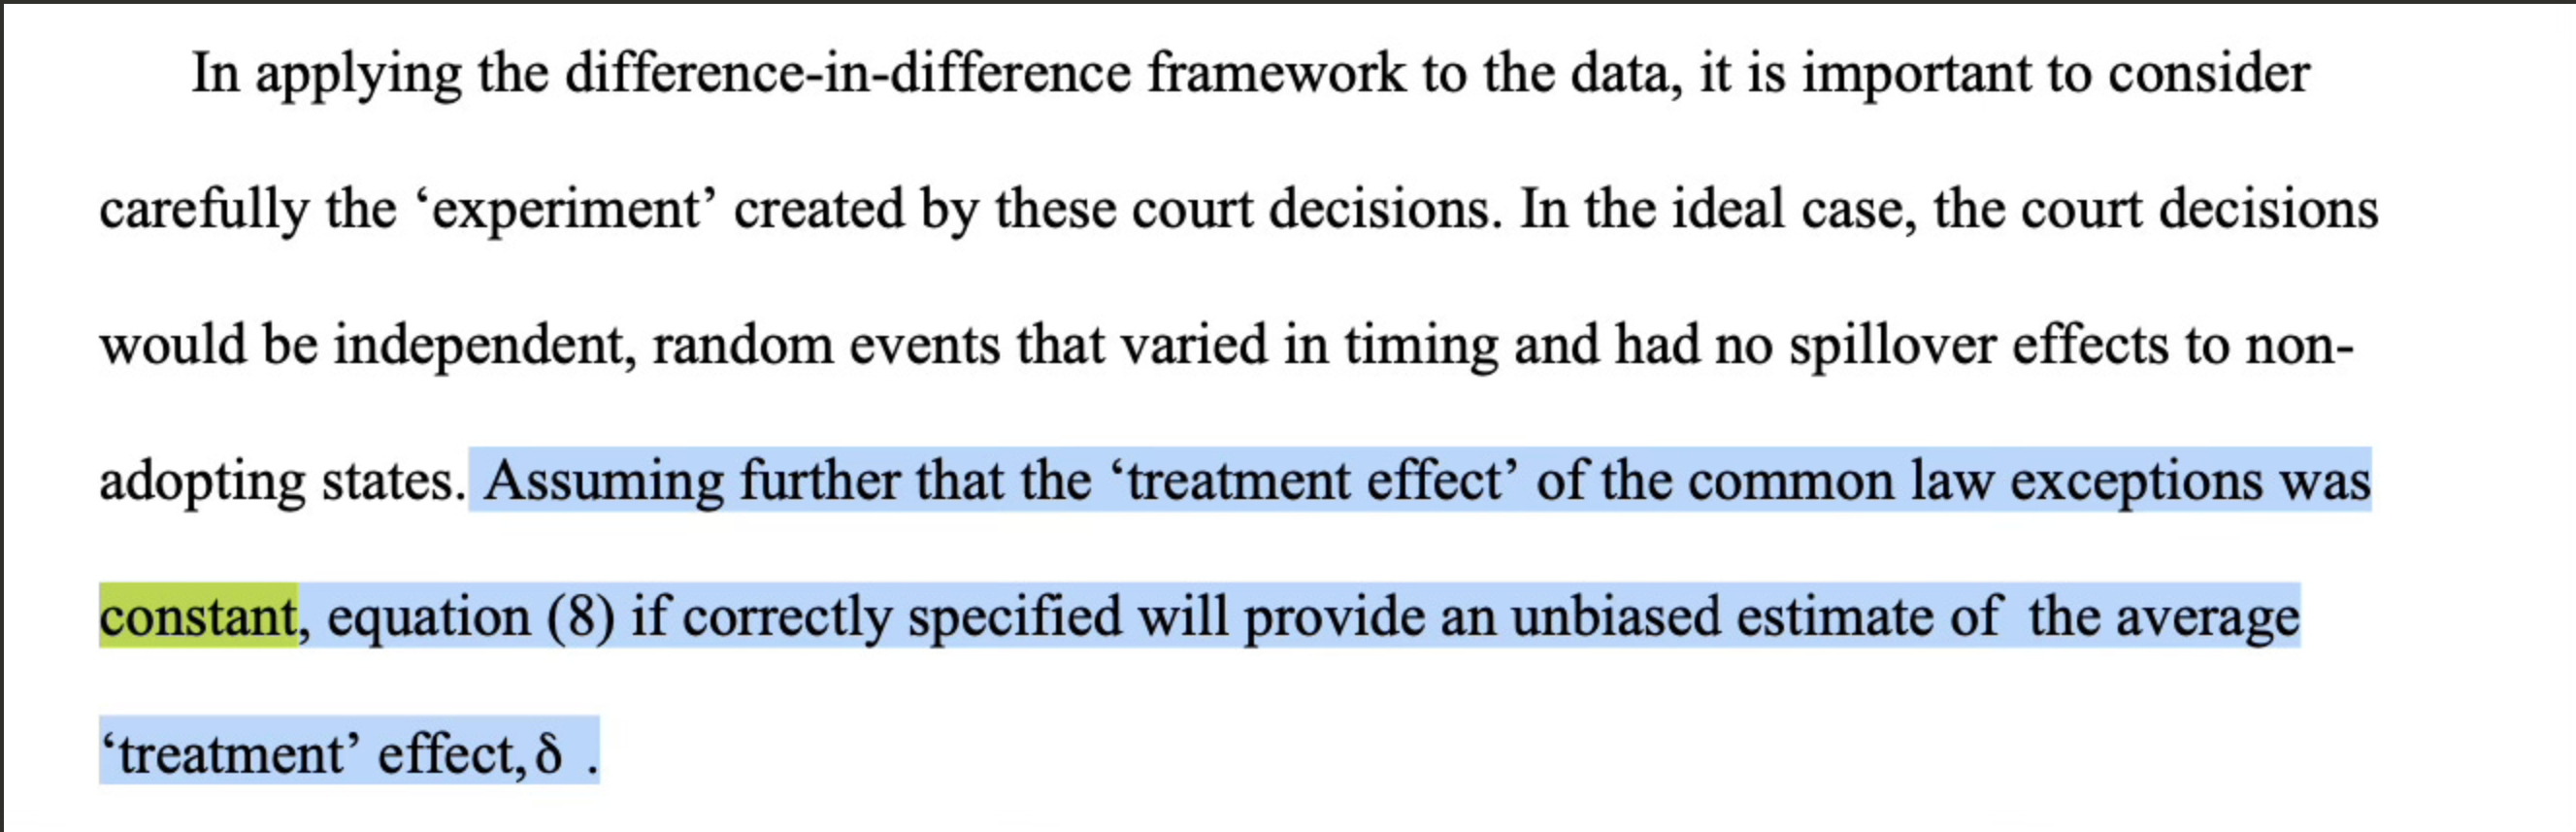
\includegraphics[scale=0.25]{./lecture_includes/autor_quote}
	\caption{David Autor clues us into the problems of TWFE}
	\end{figure}

\end{frame}









\begin{frame}{Third wave of diff-in-diff}

\begin{itemize}

\item Starts with Kirill Borusyak and Xavier Jaravel (2016) working paper posted to SSRN (later published with Jan Speiss 2023)
\item Key elements: explicit mention of the average treatment effect on the treated (ATT), heterogenous treatment effects and the pathologies of twoway fixed effects (TWFE)
\end{itemize}

\end{frame}


\begin{frame}{First Wave}

	\begin{figure}
	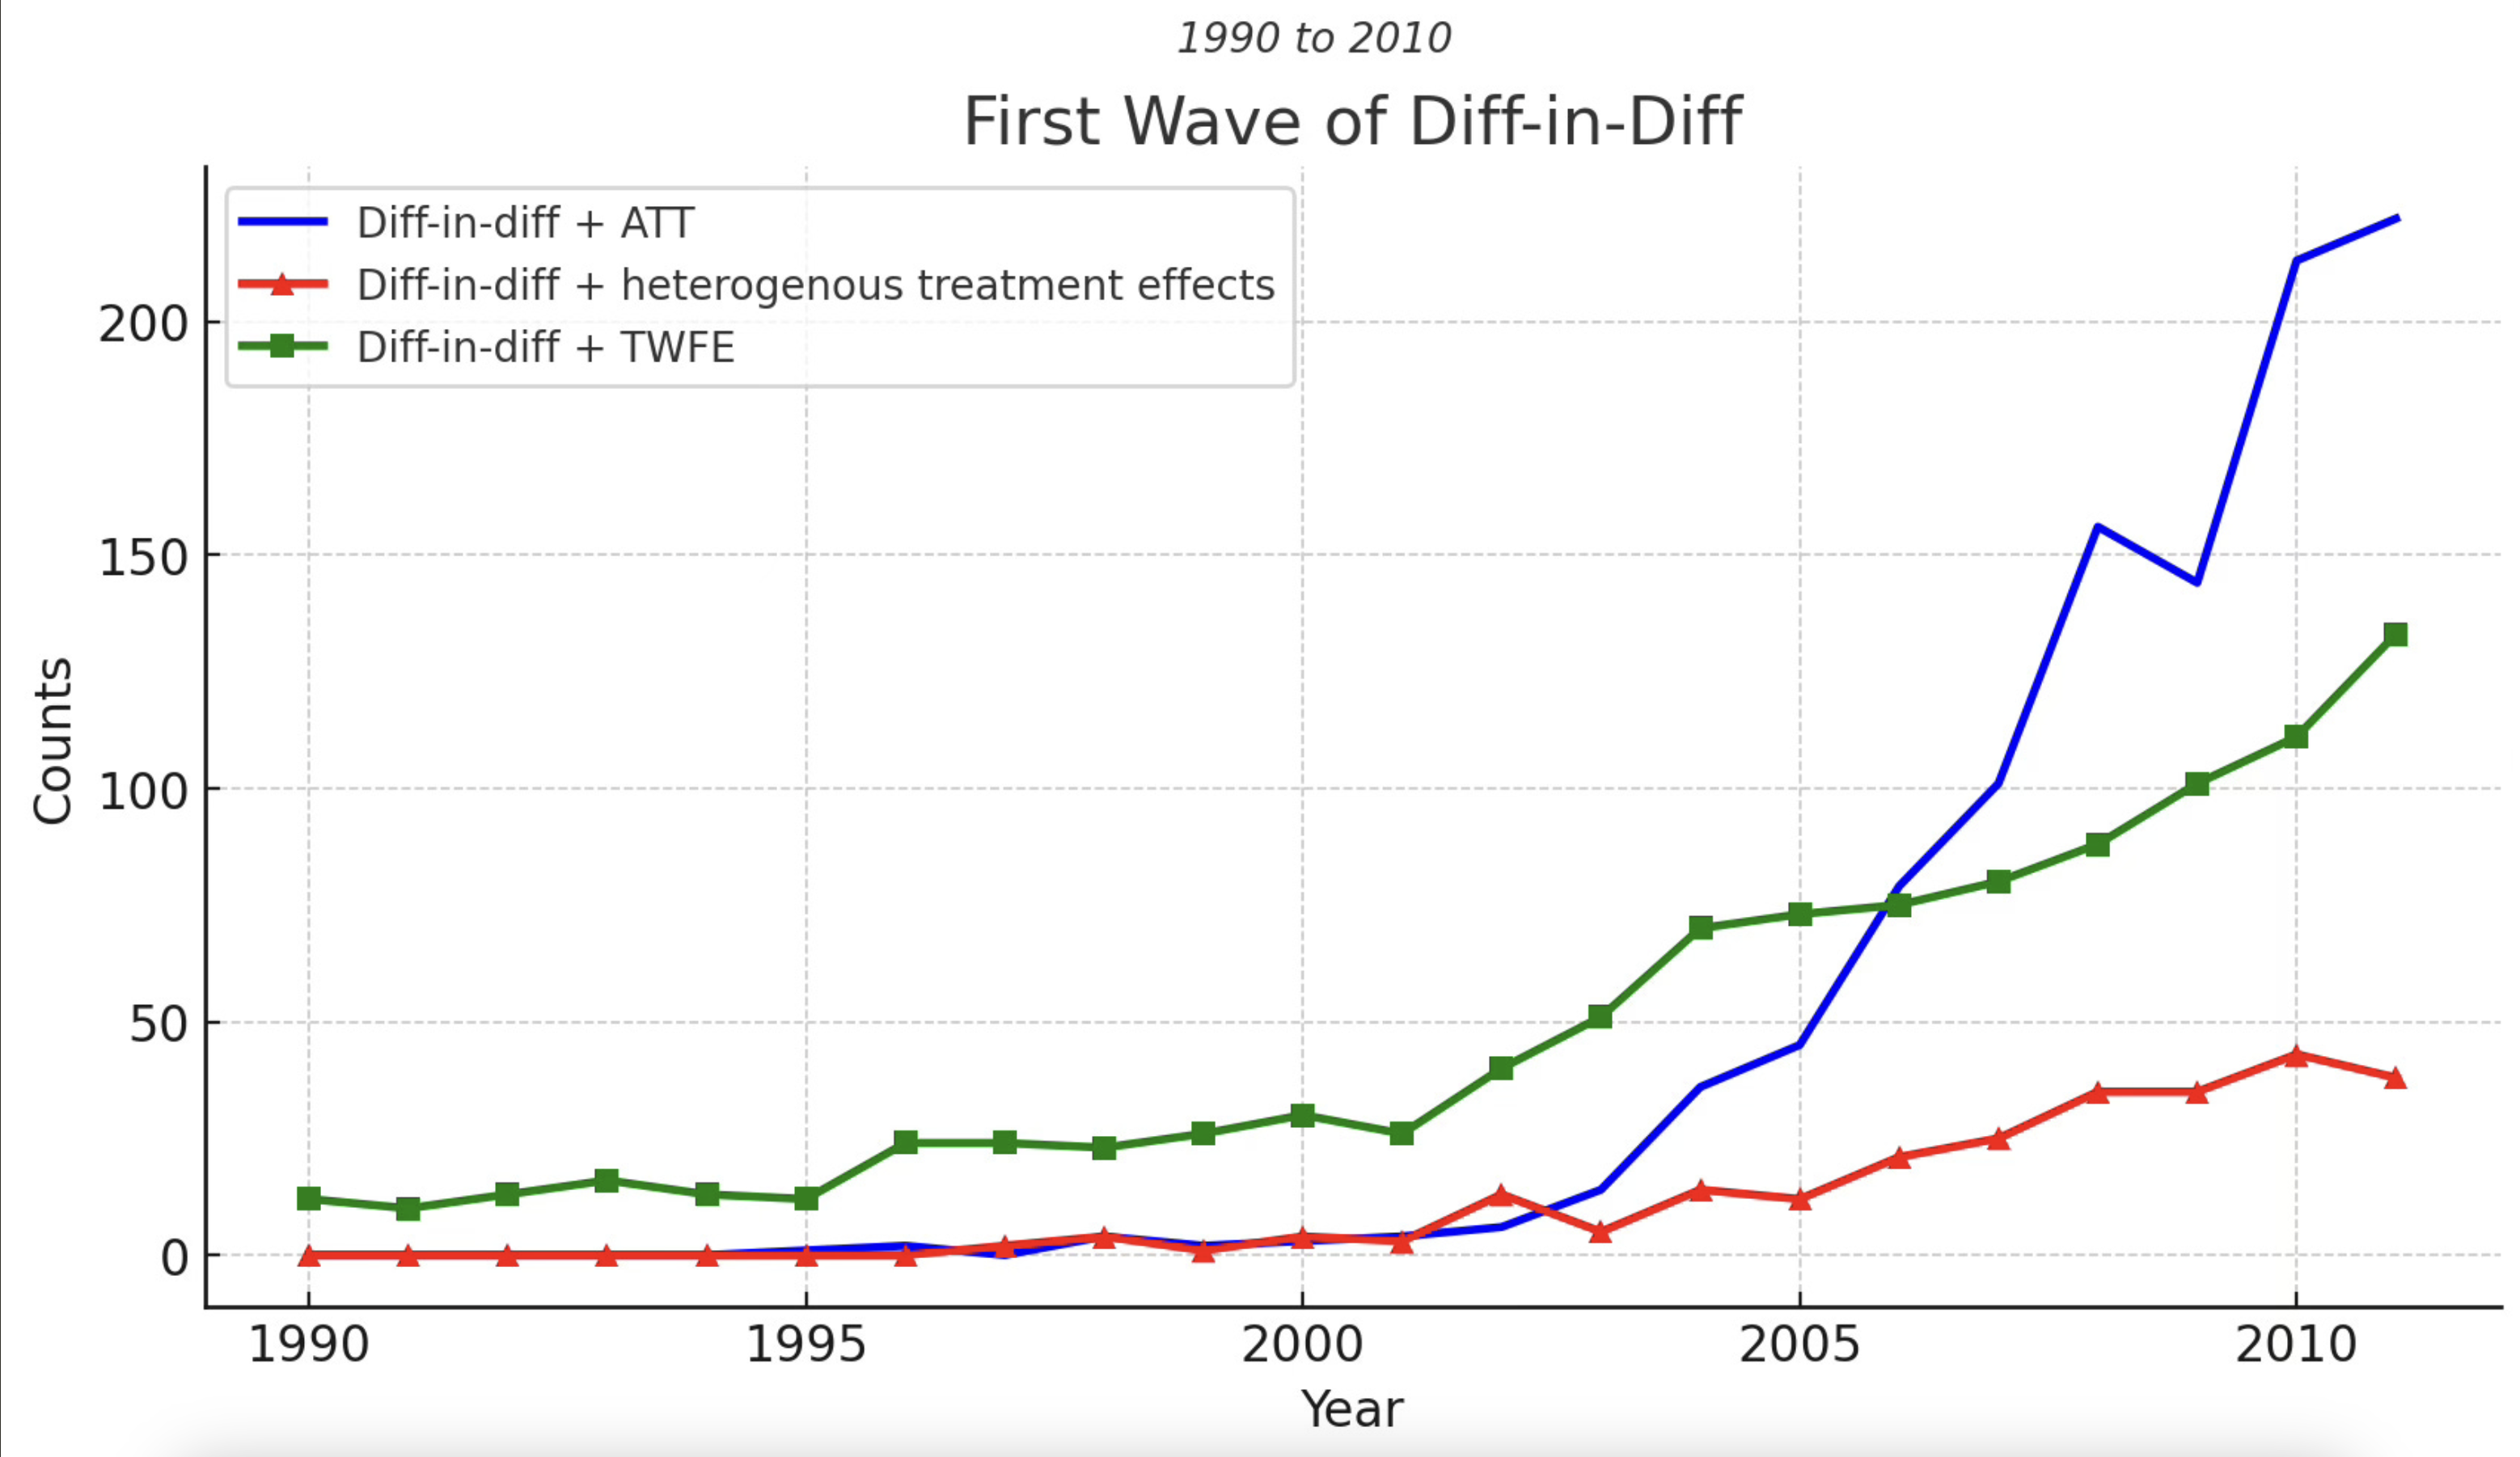
\includegraphics[scale=0.15]{./lecture_includes/wave1}
	\end{figure}

\end{frame}


\begin{frame}{Second Wave}

	\begin{figure}
	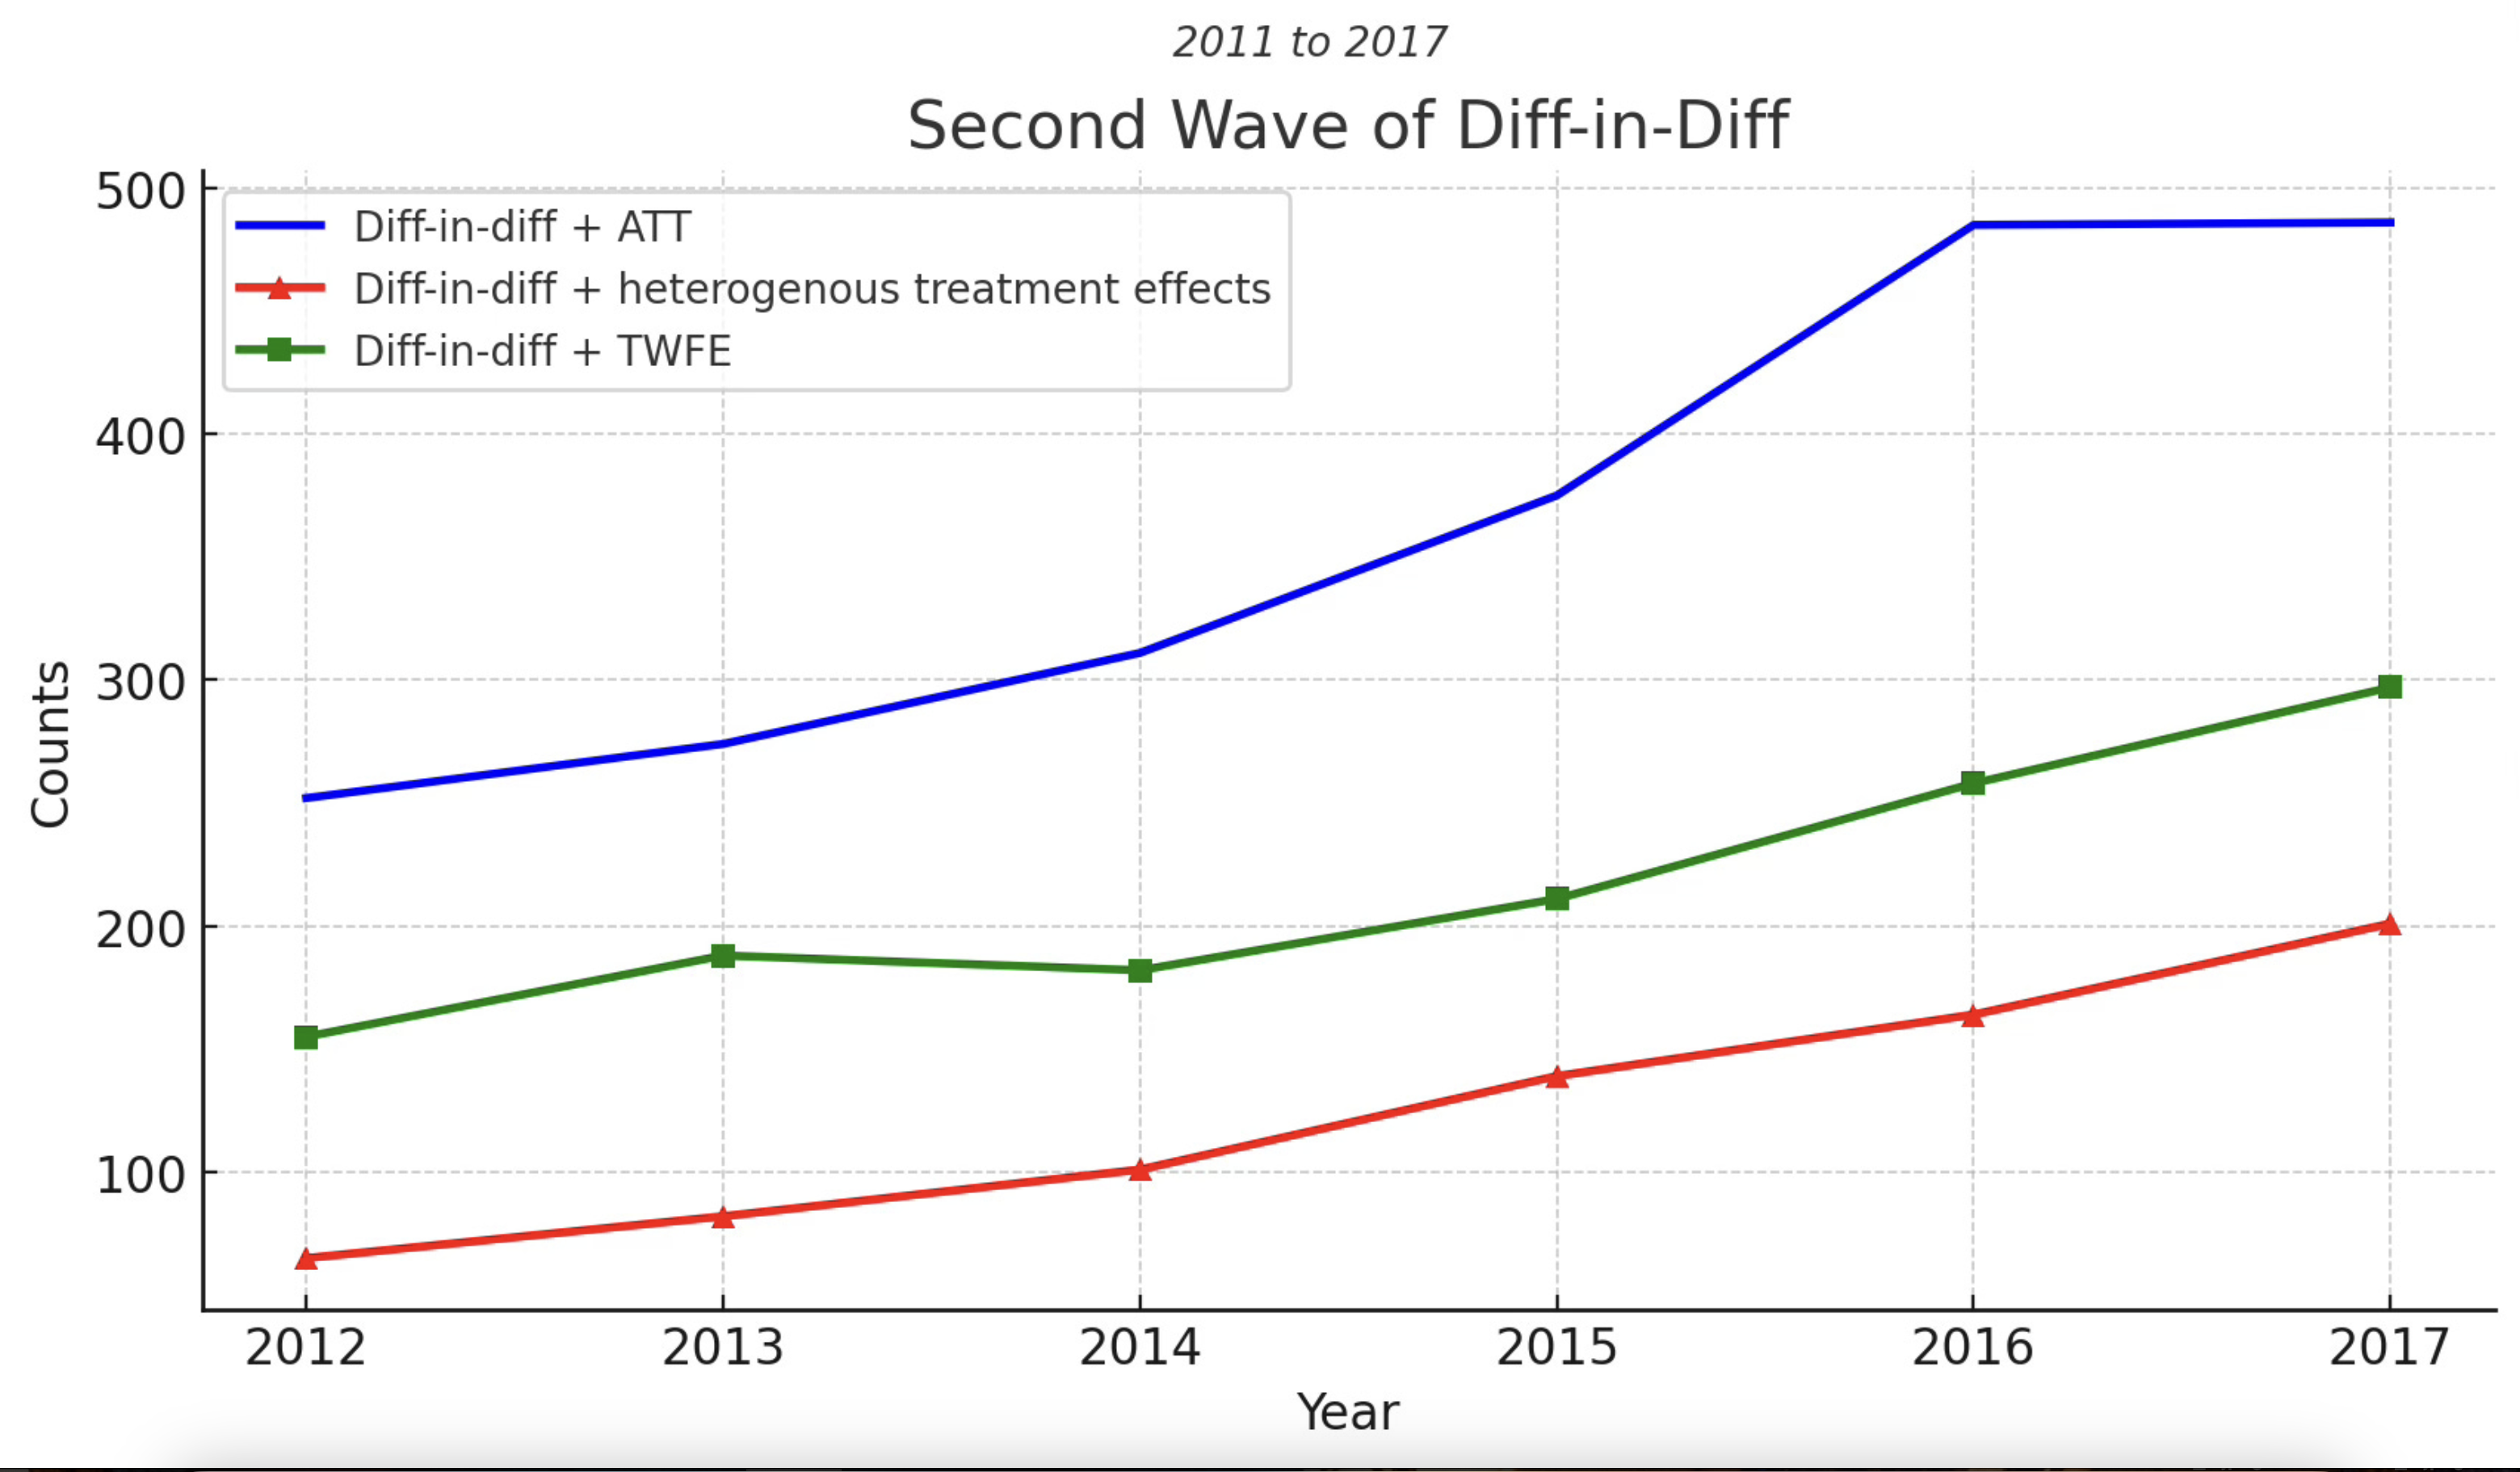
\includegraphics[scale=0.15]{./lecture_includes/wave2}
	\end{figure}

\end{frame}

\begin{frame}{Third Wave}

	\begin{figure}
	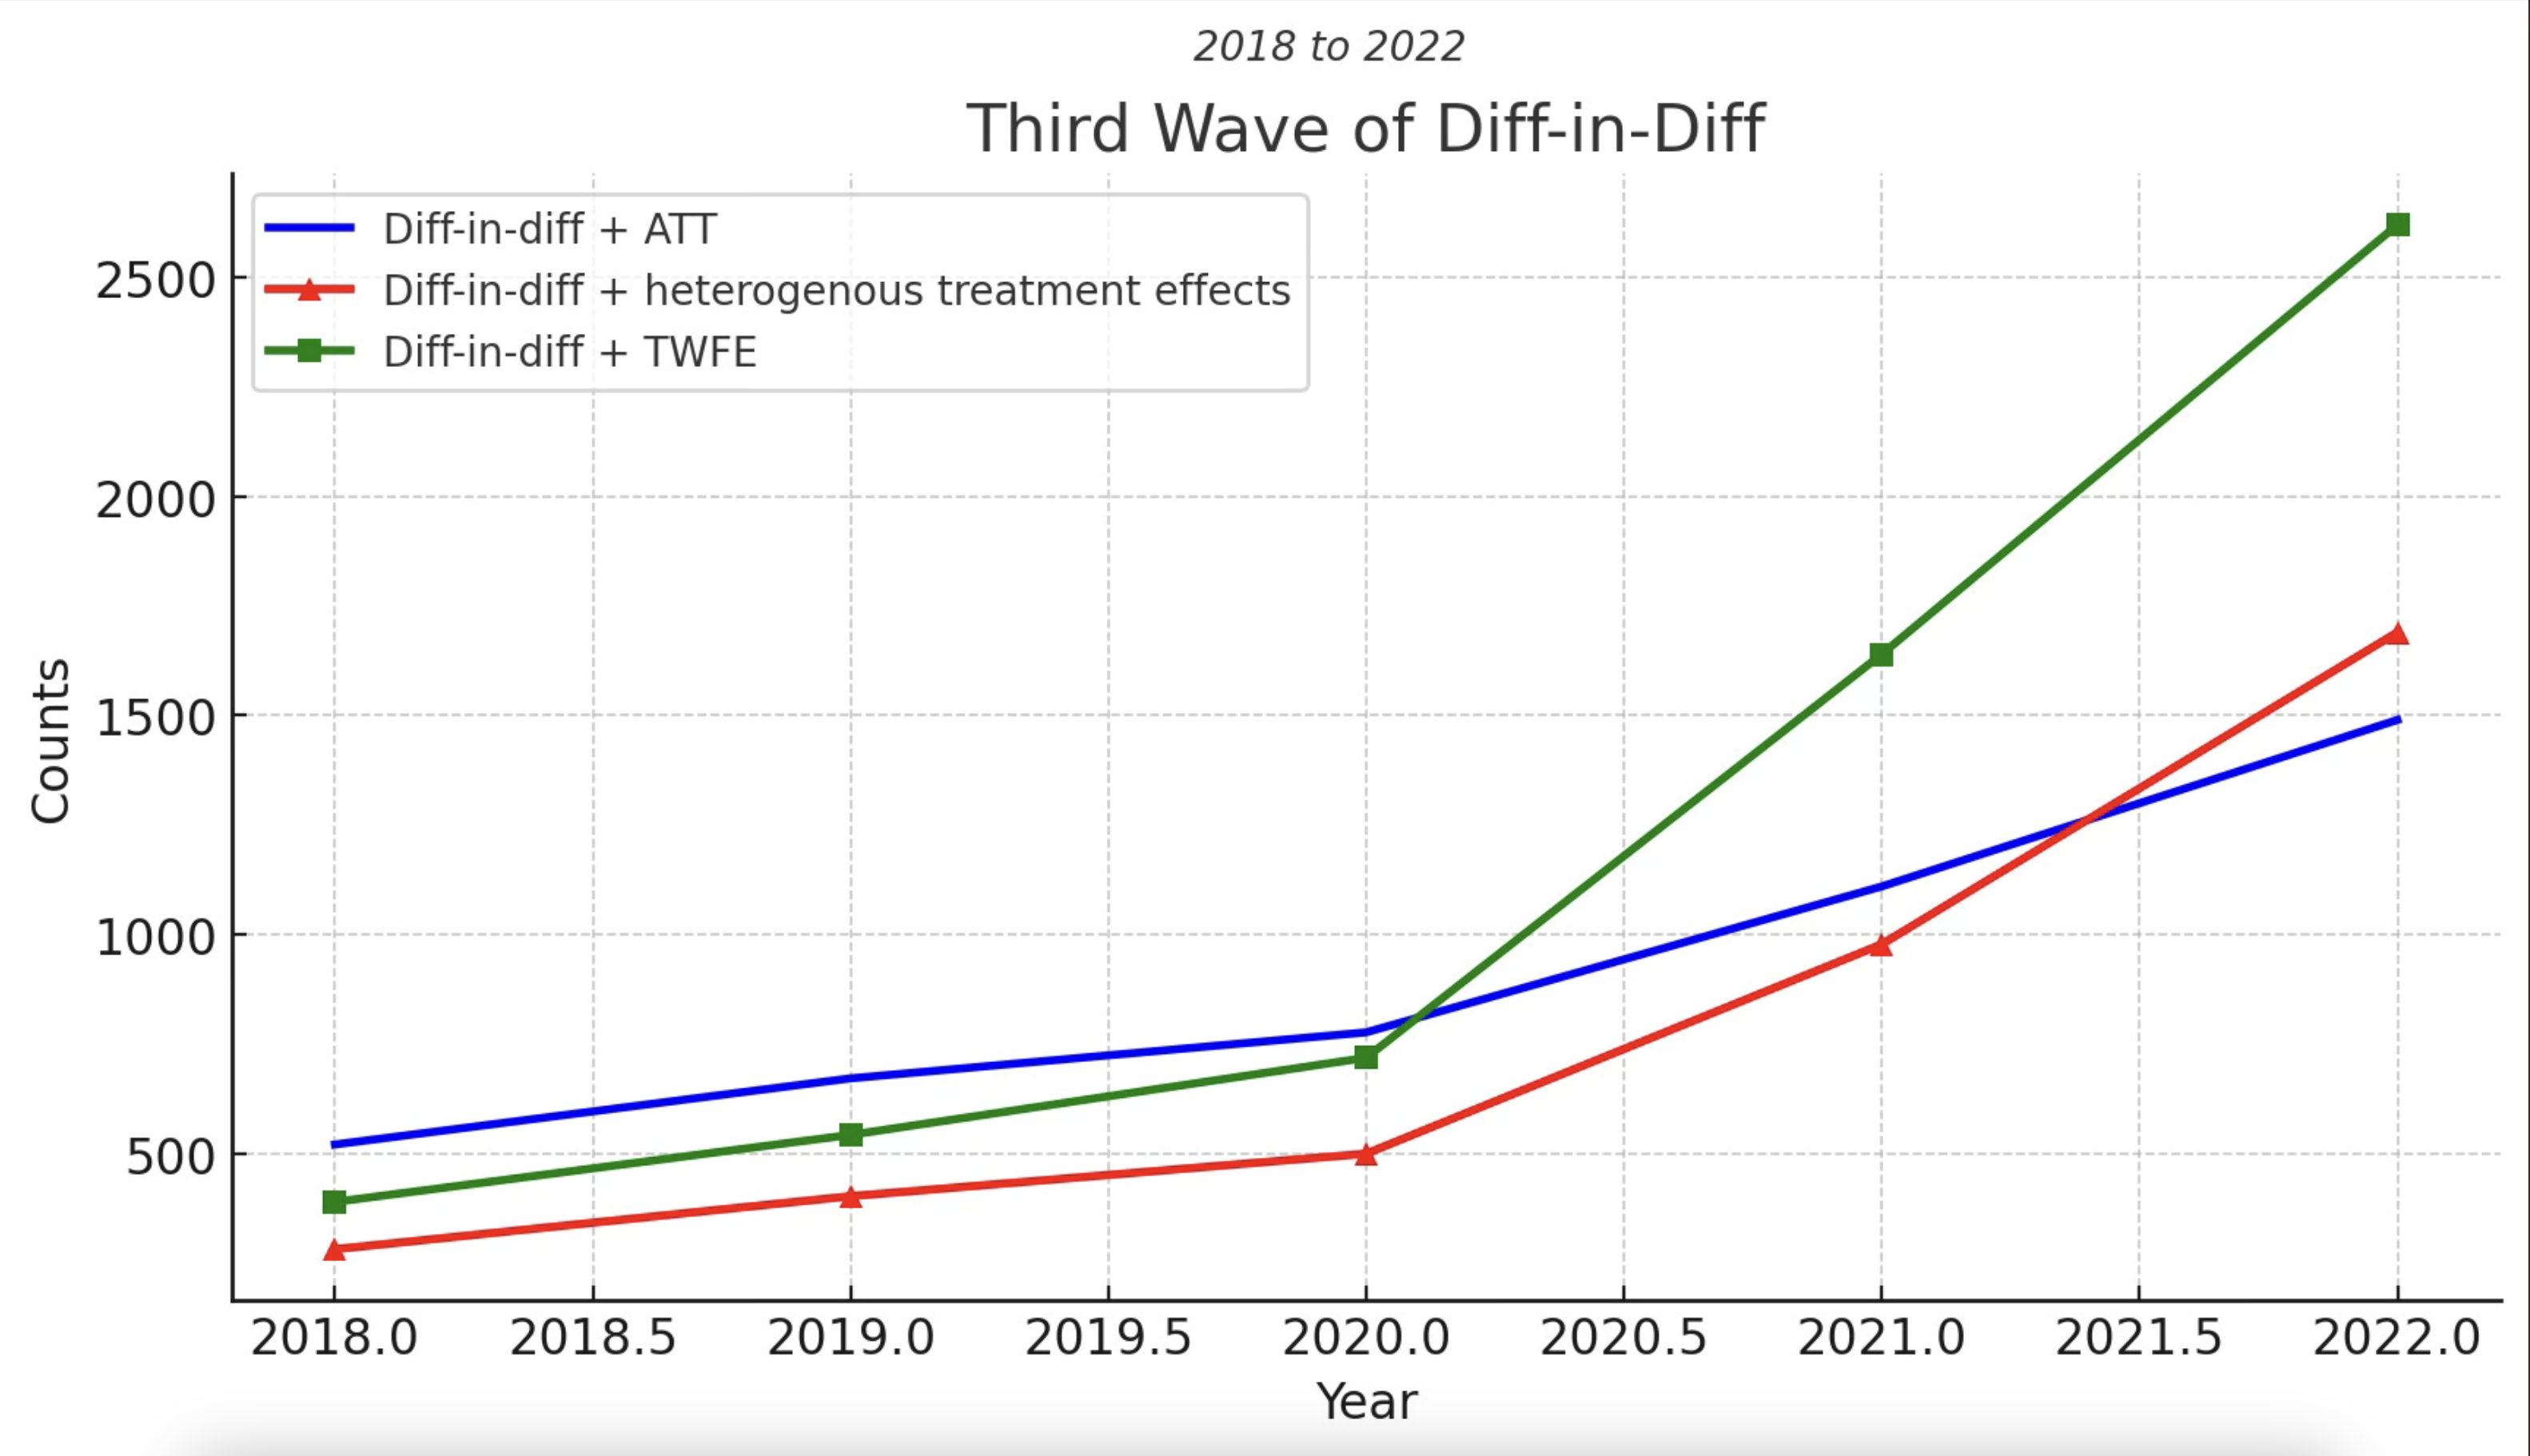
\includegraphics[scale=0.15]{./lecture_includes/wave3}
	\end{figure}

\end{frame}

\begin{frame}{TWFE relative to DID}

	\begin{figure}
	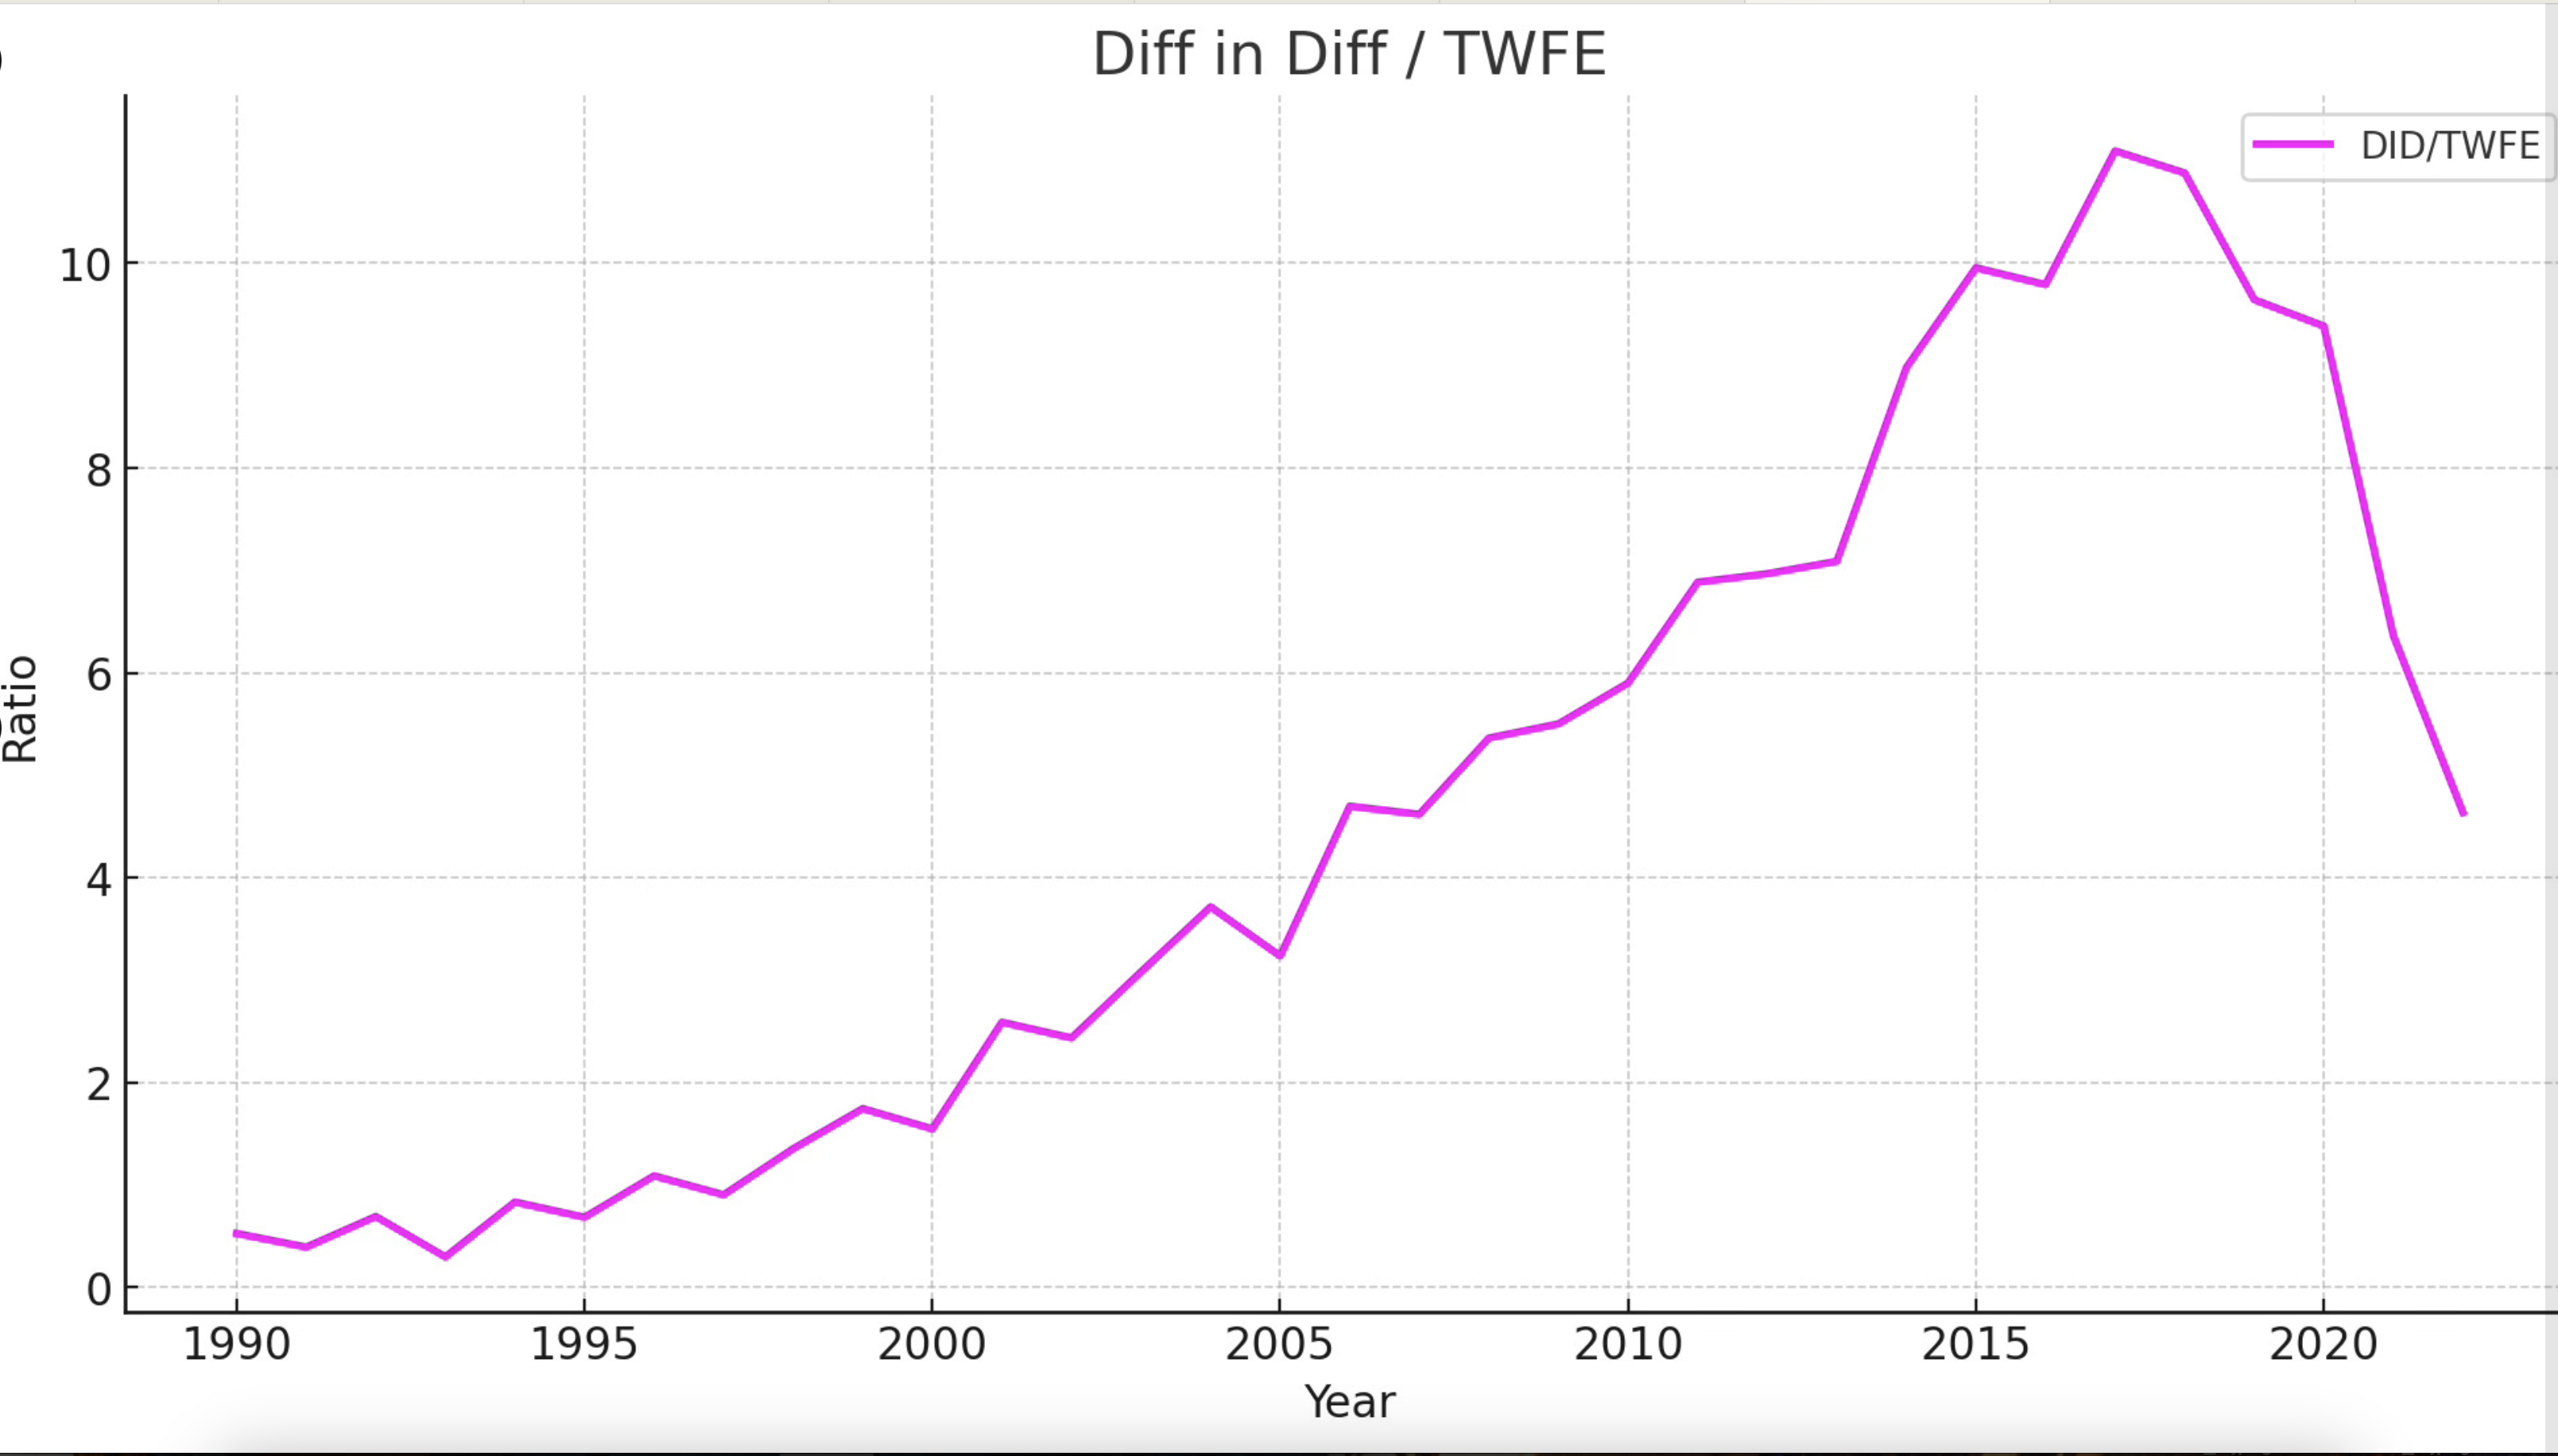
\includegraphics[scale=0.15]{./lecture_includes/wave4}
	\end{figure}

\end{frame}







\section{TWFE Pathologies}

\subsection{Historical links}




\begin{frame}{Twoway fixed effects}

\begin{itemize}
\item When working with panel data, the so-called ``twoway fixed effects'' (TWFE) estimator was the workhorse estimator
\item And from the start, regression was used with diff-in-diff, and as more complex designs began studied, panel fixed effects were a natural choice
\item But DiD is not regression, nor is it TWFE -- it is four averages and three subtractions as we saw earlier
\item Under differential timing, interpreting the TWFE coefficient became challenging given there weren't just two groups
\end{itemize}

\end{frame}

\begin{frame}{Two OLS Models}

\begin{eqnarray}
Y_{ist} &=& \alpha_0 + \alpha_1 Treat_{is} + \alpha_2 Post_{t} + \delta (Treat_{is} \times Post_t) + \varepsilon_{ist} \\
Y_{ist} &=& \beta_0 + \delta D_{ist} + \tau_t + \sigma_s + \varepsilon_{ist}
\end{eqnarray}

\bigskip

First equation is used for simple designs when everyone is treated at once; second equation was used when different groups were treated at different times (``differential timing'')

\bigskip

The coefficient on the interaction is the DiD equation of ``four averages and three subtractions'' but the coefficient on equation 2 delta under heterogenous treatment effects -- what was it?

\end{frame}


\subsection{Potential outcomes}

\begin{frame}{Equivalence}
$$Y_{ist} = \alpha_0 + \alpha_1 Treat_{is} + \alpha_2 Post_{t} + \textcolor{blue}{\delta} (Treat_{is} \times Post_t) + \varepsilon_{ist} $$

\bigskip

$$\widehat{\textcolor{blue}{\delta}} = \bigg ( \overline{y}_k^{post(k)} - \overline{y}_k^{pre(k)} \bigg ) - \bigg ( \overline{y}_U^{post(k)} - \overline{y}_U^{pre(k)} \bigg ) $$

\begin{itemize}
\item The $\delta$ in the regression is numerically identical to ``four averages and three subtractions'' 
\item And under a particular assumption, they are also unbiased estimates of an aggregate causal parameter
\item But to see this we need new notation -- potential outcomes
\end{itemize}

\end{frame}





\begin{frame}{Potential outcomes notation}
	
	\begin{itemize}
	\item Let the treatment be a binary variable: $$D_{i,t} =\begin{cases} 1 \text{ if in job training program $t$} \\ 0 \text{ if not in job training program at time $t$} \end{cases}$$where $i$ indexes an individual observation, such as a person

	\end{itemize}
\end{frame}

\begin{frame}{Potential outcomes notation}
	
	\begin{itemize}

	\item Potential outcomes: $$Y_{i,t}^j =\begin{cases} 1 \text{: wages at time $t$ if trained} \\ 0 \text{: wages at time $t$ if not trained} \end{cases}$$where $j$ indexes a counterfactual state of the world

	\end{itemize}
\end{frame}



\begin{frame}{Treatment effect definitions}


	\begin{block}{Individual treatment effect}
	    The individual treatment effect,  $\delta_i$, equals $Y_i^1-Y_i^0$
	\end{block}

Missing data problem:  I don't know my own counterfactual
	
\end{frame}


\begin{frame}{Conditional Average Treatment Effects}	
	\begin{block}{Average Treatment Effect on the Treated (ATT)}
	The average treatment effect on the treatment group is equal to the average treatment effect conditional on being a treatment group member:
		\begin{eqnarray*}
		E[\delta|D=1]&=&E[Y^1-Y^0|D=1] \nonumber \\
		&=&E[Y^1|D=1]-\textcolor{red}{E[Y^0|D=1]}
		\end{eqnarray*}
	\end{block}
	
	\bigskip

This is one of the most important policy parameters, if not the most important, and coincidentally it's also the parameter you get with diff-in-diff (even with heterogeneity)

	
\end{frame}

\begin{frame}{Potential outcomes vs data}

\begin{itemize}
\item ATT is expressed in terms of potential outcomes, but we do not use potential outcomes for estimation; we use data
\item Potential outcomes are unknown and \emph{hypothetical} possibilities describing states of the world but our data are realized outcomes, or ``data'', that actually occurred
\item Potential outcomes become realized under treatment assignment $$Y_{it}=D_{it}Y_{it}^1 + (1-D_{it})Y_{it}^0$$
\item Depending on how the treatment is assigned really dictates whether correlations reveal causal effects or bias

\end{itemize}
\end{frame}




\begin{frame}{DiD equation}

Orley's ``four averages and three subtractions'', or what Bacon will call the 2x2

\begin{eqnarray*}
\widehat{\delta} = \bigg ( E[Y_k|Post] - E[Y_k|Pre] \bigg ) - \bigg ( E[Y_U | Post ] - E[ Y_U | Pre] \bigg) \\
\end{eqnarray*}$k$ are the people in the job training program, $U$ are the untreated people not in the program, $Post$ is after the trainees took the class, $Pre$ is the period just before they took the class, and $E[y]$ is mean earnings. 

\bigskip

Does $\widehat{\delta}$ equal the ATT?  If so when? If not why not?

\end{frame}



\begin{frame}{Potential outcomes and the switching equation}

\begin{eqnarray*}
\widehat{\delta} &=& \bigg ( \underbrace{E[Y^1_k|Post] - E[Y^0_k|Pre] \bigg ) - \bigg ( E[Y^0_U | Post ] - E[ Y^0_U | Pre]}_{\mathclap{\text{Switching equation}}} \bigg)  \\
&&+ \underbrace{\textcolor{red}{E[Y_k^0 |Post] - E[Y^0_k | Post]}}_{\mathclap{\text{Adding zero}}} 
\end{eqnarray*}

\end{frame}

\begin{frame}{Parallel trends bias}

\begin{eqnarray*}
\widehat{\delta} &=& \underbrace{E[Y^1_k | Post] - \textcolor{red}{E[Y^0_k | Post]}}_{\mathclap{\text{ATT}}} \\
&& + \bigg [  \underbrace{\textcolor{red}{E[Y^0_k | Post]} - E[Y^0_k | Pre] \bigg ] - \bigg [ E[Y^0_U | Post] - E[Y_U^0 | Pre] }_{\mathclap{\text{Non-parallel trends bias in 2x2 case}}} \bigg ]
\end{eqnarray*}


\end{frame}

\begin{frame}{Identification through parallel trends}
	

	\begin{block}{Parallel trends}
	Assume two groups, treated and comparison group, then we define parallel trends as:	 $$\textcolor{red}{E(}\textcolor{red}{\Delta Y^0_k)} = E(\Delta Y^0_U)$$
	\end{block}

\textbf{In words}: ``The \textcolor{red}{evolution of earnings for our trainees \emph{had they not trained}} is the same as the evolution of mean earnings for non-trainees''.  

\bigskip

It's in \textcolor{red}{red} because parallel trends is untestable and critically important to estimation of the ATT using any method, OLS or ``four averages and three subtractions''

	

	
\end{frame}














\subsection{Bacon decomposition}

\begin{frame}{Discussion of estimate}


$$Y_{ist} = \beta_0 + \delta D_{ist} + \tau_t + \sigma_s + \varepsilon_{ist}$$


\begin{itemize}
\item So that's the simple case; what about the differential timing case?  

\item If you estimate with OLS with differential timing, what does $\widehat{\delta}$ correspond to?
\item It relates to the previous ``four averages and three subtractions'' -- but it's numerous of them, not just one
\item In differential timing, the coefficient, $\widehat{\delta}^{TWFE}$, is a weighted average of \emph{all} possible DiD calculations -- including some we should not be calculating

\end{itemize}

\end{frame}






\begin{frame}{$K^2$ distinct DDs}

Let's look at 3 timing groups (a, b and c) and one untreated group (U).  With 3 timing groups, there are 9 2x2 DDs.  Here they are:


\begin{center}
\begin{tabular}{c|c|c}
\multicolumn{1}{l}{} &
\multicolumn{1}{l}{} &
\multicolumn{1}{l}{} \\
\midrule
a to b & b to a & c to a \\
a to c & b to c & c to b \\
a to U & b to U & c to U \\
\midrule
\end{tabular}
\end{center}

\bigskip

Let's return to a simpler example with only two groups -- a $k$ group treated at $t_k^*$ and an $l$ treated at $t_l^*$ plus an never-treated group called the $U$ untreated group
\end{frame} 


\begin{frame}{Terms and notation}

\begin{itemize}
\item Let there be two treatment groups (k,l) and one untreated group (U)
\item k,l define the groups based on when they receive treatment (differently in time) with k receiving it earlier than l
\item Denote $\overline{D}_k$ as the share of time each group spends in treatment status
\item Denote $\widehat{\delta}_{jb}^{2x2}$ as the canonical $2\times 2$ DD estimator for groups $j$ and b where $j$ is the treatment group and $b$ is the comparison group
\end{itemize}

\end{frame}


\imageframe{./lecture_includes/bacon_goodman_2.png}



\begin{frame}[plain]
$$\widehat{\delta}^{2x2}_{kU} = \bigg ( \overline{y}_k^{post(k)} - \overline{y}_k^{pre(k)} \bigg ) - \bigg ( \overline{y}_U^{post(k)} - \overline{y}_U^{pre(k)} \bigg ) $$
	\begin{figure}
	\includegraphics[scale=0.45]{./lecture_includes/bacon_goodman_3.png}
	\end{figure}

\end{frame}

\begin{frame}[plain]
$$\widehat{\delta}^{2x2}_{lU} = \bigg ( \overline{y}_l^{post(l)} - \overline{y}_l^{pre(l)} \bigg ) - \bigg ( \overline{y}_U^{post(l)} - \overline{y}_U^{pre(l)} \bigg ) $$
	\begin{figure}
	\includegraphics[scale=0.45]{./lecture_includes/bacon_goodman_4.png}
	\end{figure}

\end{frame}


\begin{frame}[plain]

$$\delta_{kl}^{2x2,k} = \bigg ( \overline{y}_k^{MID(k,l)} - \overline{y}_k^{Pre(k,l)} \bigg ) - \bigg ( \overline{y}_l^{MID(k,l)} - \overline{y}_l^{PRE(k,l)} \bigg ) $$

	\begin{figure}
	\includegraphics[scale=0.45]{./lecture_includes/bacon_goodman_6.png}
	\end{figure}

\end{frame}

\begin{frame}[plain]
$$\delta_{lk}^{2x2,l} = \bigg ( \overline{y}_l^{POST(k,l)} - \overline{y}_l^{MID(k,l)} \bigg ) - \bigg ( \overline{y}_k^{POST(k,l)} - \overline{y}_k^{MID(k,l)} \bigg ) $$

	\begin{figure}
	\includegraphics[scale=0.4]{./lecture_includes/bacon_goodman_7.png}
	\end{figure}

\end{frame}


	

\begin{frame}{Bacon decomposition}

$$Y_{ist} = \beta_0 + \delta D_{ist} + \tau_t + \sigma_s + \varepsilon_{ist}$$


TWFE estimate of $\widehat{\delta}$ is equal to a weighted average over all group 2x2 (of which there are 4 in this example)
\begin{eqnarray*}	
\widehat{\delta}^{TWFE} = \sum_{k \neq U} s_{kU}\widehat{\delta}_{kU}^{2x2} + \sum_{k \neq U} \sum_{l>k} s_{kl}  \bigg [ \mu_{kl}\widehat{\delta}_{kl}^{2x2,k} + (1-\mu_{kl}) \widehat{\delta}_{lk}^{2x2,l} \bigg]
\end{eqnarray*}where that first 2x2 combines the k compared to U and the l to U (combined to make the equation shorter)

\end{frame}
	


\begin{frame}{Third, the Weights}

 \begin{eqnarray*} s_{ku} &=& \frac{ n_k n_u \overline{D}_k (1- \overline{D}_k ) }{ \widehat{Var} ( \tilde{D}_{it} )} \\
s_{kl} &=& \frac{ n_k n_l (\overline{D}_k - \overline{D}_{l} ) ( 1- ( \overline{D}_k - \overline{D}_{l} )) }{\widehat{Var}(\tilde{D}_{it})} \\
\mu_{kl} &=& \frac{1 - \overline{D}_k }{1 - ( \overline{D}_k - \overline{D}_{l} )}
\end{eqnarray*}where $n$ refer to sample sizes, $\overline{D}_k (1- \overline{D}_k )$ $(\overline{D}_k - \overline{D}_{l} ) ( 1- ( \overline{D}_k - \overline{D}_{l} ))$ expressions refer to variance of treatment, and the final equation is the same for two timing groups.

\end{frame}

\begin{frame}{Weights discussion}

\begin{itemize}
\item Two things to note:
	\begin{itemize}
	\item More units in a group, the bigger its 2x2 weight is
	\item Group treatment variance weights up or down a group's 2x2
	\end{itemize}
\item Think about what causes the treatment variance to be as big as possible. Let's think about the $s_{ku}$ weights.
	\begin{itemize}
	\item $\overline{D}=0.1$. Then $0.1 \times 0.9 = 0.09$
	\item $\overline{D}=0.4$. Then $0.4 \times 0.6 =0.24$
	\item $\overline{D}=0.5$. Then $0.5 \times 0.5 = 0.25$
	\item $\overline{D}=0.6$. Then $0.6 \times 0.4 = 0.24$
	\end{itemize}
\item This means the weight on treatment variance is maximized for \emph{groups treated in middle of the panel}
\end{itemize}
\end{frame}

\begin{frame}{More weights discussion}

\begin{itemize}
\item But what about the ``treated on treated'' weights (i.e., $\overline{D}_k - \overline{D}_{l} $)  
\item Same principle as before - when the difference between treatment variance is close to 0.5, those 2x2s are given the greatest weight
\item For instance, say $t^*_k=0.15$ and $t^*_l=0.67$. Then $\overline{D}_k - \overline{D}_{l} = 0.52$.  And thus $0.52 \times 0.48 = 0.2496$.
\end{itemize}

\end{frame}


\begin{frame}{Summarizing TWFE centralities}

\begin{itemize}
\item Groups in the middle of the panel weight up their respective 2x2s via the variance weighting
\item Decomposition highlights the strange role of panel length when using TWFE
\item Different choices about panel length change both the 2x2 and the weights based on variance of treatment
\end{itemize}

\end{frame}




\begin{frame}{Back to TWFE}


$$Y_{ist} = \beta_0 + \delta D_{ist} + \tau_t + \sigma_s + \varepsilon_{ist}$$


\begin{itemize}

\item So we know that the estimate is a weighted average over all ``four averages and three subtractions'' but is that good or bad?
\item It's good if it's unbiased; it's bad if it isn't, and the decomposition doesn't tell us which unless we replace realized outcomes with potential outcomes
\item Bacon shows that TWFE estimate of $\delta$ needs two assumptions for unbiasedness:
	\begin{enumerate}
	\item variance weighted parallel trends are zero and 
	\item no dynamic treatment effects (not the case with 2x2)
	\end{enumerate}
\item Under those assumptions, TWFE estimator estimates the variance weighted ATT as a weighted average of all possible ATTs (not just weighted average of DiDs)

\end{itemize}

\end{frame}


\begin{frame}{Moving from 2x2s to causal effects and bias terms}

Let's start breaking down these estimators into their corresponding estimation objects expressed in causal effects and biases


\begin{eqnarray*}
\widehat{\delta}^{2x2}_{kU} &=& ATT_k{Post} + \Delta Y^0_k(Post(k),Pre(k)) - \Delta Y^0_U(Post(k),Pre) \\
\widehat{\delta}^{2x2}_{kl} &=& ATT_k(MID) + \Delta Y^0_k(MID,Pre) - \Delta Y^0_l(MID, Pre)
\end{eqnarray*}These look the same because you're always comparing the treated unit with an untreated unit (though in the second case it's just that they haven't been treated \emph{yet}). 

\end{frame}

\begin{frame}{The dangerous 2x2}

But what about the 2x2 that compared the late groups to the already-treated earlier groups? With a lot of substitutions we get:

\begin{eqnarray*}
\widehat{\delta}^{2x2}_{lk} &=& ATT_{l,Post(l)} + \underbrace{\Delta Y^0_l(Post(l),MID) - \Delta Y^0_k ( Post(l), MID)}_{\mathclap{\text{Parallel trends bias}}} \\
&& - \underbrace{(ATT_k(Post) - ATT_k(Mid))}_{\mathclap{\text{Heterogeneity bias!}}}
\end{eqnarray*}


\end{frame}

\begin{frame}{Substitute all this stuff into the decomposition formula}

\begin{eqnarray*}	
\widehat{\delta}^{DD} = \sum_{k \neq U} s_{kU}\widehat{\delta}_{kU}^{2x2} + \sum_{k \neq U} \sum_{l>k} s_{kl}  \bigg [ \mu_{kl}\widehat{\delta}_{kl}^{2x2,k} + (1-\mu_{kl}) \widehat{\delta}_{kl}^{2x2,l} \bigg]
\end{eqnarray*}where we will make these substitutions\begin{eqnarray*}
\widehat{\delta}_{kU}^{2x2} &=& ATT_k(Post) + \Delta Y_l^0(Post,Pre) - \Delta Y_U^0(Post, Pre) \\
\widehat{\delta}_{kl}^{2x2,k} &=& ATT_k(Mid) + \Delta Y_l^0(Mid,Pre) - \Delta Y_l^0(Mid, Pre) \\
\widehat{\delta}^{2x2,l}_{lk} &=& ATT_{l}Post(l) + \Delta Y^0_l(Post(l),MID) - \Delta Y^0_k ( Post(l), MID) \\
&&- (ATT_k(Post) - ATT_k(Mid))
\end{eqnarray*}Notice all those potential sources of biases! 

\end{frame}


\begin{frame}{Potential Outcome Notation}

\begin{eqnarray*}
p\text{ }lim\text{ } \widehat{\delta}^{TWFE}_{n\to\infty} &=& VWATT + VWPT - \Delta ATT
\end{eqnarray*}

\begin{itemize}
\item Notice the number of assumptions needed \emph{even} to estimate this very strange weighted ATT (which is a function of how you drew the panel in the first place). 
\item With dynamics, it attenuates the estimate (bias) and can even reverse sign depending on the magnitudes of what is otherwise effects in the sign in a reinforcing direction! 
\item Model can flip signs (does not satisfy a ``no sign flip property'')
\end{itemize}

\end{frame}



\subsection{Simulation}



\begin{frame}{Simulated data}

\begin{itemize}
\item 1000 firms, 40 states, 25 firms per states, 1980 to 2009 or 30 years, 30,000 observations, four groups

\item I'll impose ``unit level parallel trends'', which is much stronger than we need (we only need average parallel trends)

\item Also no anticipation of treatment effects until treatment occurs but does \emph{not} guarantee homogenous treatment effects

\item Two types of situations: constant versus dynamic treatment effects
\end{itemize}
\end{frame}



\begin{frame}{Constant vs Dynamic Treatment Effects}
    \begin{columns}
        \column{0.5\linewidth}
        \centering
        \includegraphics[height=6.5cm, width=5.5cm]{./lecture_includes/constant_te}

        \column{0.5\linewidth}
        \centering
        \includegraphics[height=6.5cm, width=5.5cm]{./lecture_includes/dynamic_te}
    \end{columns} 
\end{frame}




\begin{frame}{Group-time ATT}
       \begin{columns}
          \column{0.38\linewidth}
             \centering
             \includegraphics[height=6.5cm, width=5.5cm]{./lecture_includes/baker_attgt}
           \column{0.48\linewidth}
		\begin{itemize}
\item Heterogenous treatment effects across time and across groups
\item Cells are called ``group-time ATT'' (Callaway and Sant'anna 2020) or ``cohort ATT'' (Sun and Abraham 2020)
\item ATT is weighted average of all cells and $+82$ with uniform weights $1/60$
		\end{itemize}
         \end{columns} 
    \end{frame}

\begin{frame}{Estimation}

\bigskip

Estimate the following equation using OLS:

$$Y_{ist} = \alpha_i + \gamma_t +\delta D_{it} + \varepsilon_{ist}$$


\begin{table}[htbp]\centering
\small
\caption{Estimating ATT with different models}
\begin{center}
\begin{tabular}{l*{5}{c}}
\hline
\multicolumn{1}{l}{\textbf{}}&
\multicolumn{1}{c}{\textbf{Truth}}&
\multicolumn{1}{c}{\textbf{(TWFE)}}&
\multicolumn{1}{c}{\textbf{(CS)}}&
\multicolumn{1}{c}{\textbf{(SA)}}&
\multicolumn{1}{c}{\textbf{(BJS)}}\\
\hline
$\widehat{ATT}$  & 82    & -6.69*** &&&\\
\hline
\end{tabular}
\end{center}
\end{table}

The sign flipped.  Why?  Because of \emph{extreme} dynamics (i.e., $- \Delta ATT$)

\end{frame}

\begin{frame}{Bacon decomposition}
\begin{table}[htbp]\centering
\small
\caption{Bacon Decomposition (TWFE $= -6.69$)}
\begin{center}
\begin{tabular}{l*{5}{c}}
\hline
\multicolumn{1}{l}{\textbf{DD Comparison}}&
\multicolumn{1}{l}{\textbf{Weight}}&
\multicolumn{1}{l}{\textbf{Avg DD Est}}\\
\hline
Earlier T vs. Later C  &     0.500   &       51.800 \\
Later T vs. Earlier C   &    0.500    &     -65.180 \\
\midrule
T $=$ Treatment; C$ =$ Comparison \\
$(0.5*51.8) + (0.5*-65.180) = -6.69$ \\
\hline
\end{tabular}
\end{center}
\end{table}

\bigskip

While large weight on the ``late to early 2x2'' is \emph{suggestive} of an issue, these would appear even if we had constant treatment effects

\end{frame}






\section{Two solutions and a new decomposition}

\subsection{CS}



\begin{frame}{Robust DiD}

\begin{itemize}

\item There are probably about 6-8 possible robust DiD methods that can be used now
\item All of them have certain things in common -- don't use already treated units as controls
\item To review all of them is impossible in a short class so I will focus on two
\item Callaway and Sant'Anna (CS) and Sun and Abraham (SA), but I will point you to more

\end{itemize}

\end{frame}

\begin{frame}{Callaway and Sant'Anna}



CS is a DiD estimator used for estimating and then summarizing specific ATT parameters for each treatment group for each period (``group-time ATT'') under differential timing assuming SUTVA, no anticipation, common support and conditional parallel trends

\bigskip

CS is a straightforward estimator -- identify smaller causal effects per group and time (``building blocks'') and then aggregate them into whatever parameter you're interested in using non-negative weights while avoiding ``bad controls''



\end{frame}


\begin{frame}{Examples of when you'd use it}

\begin{enumerate}
\item When treatment effects differ depending on when it was adopted
\item When treatment effects change over time
\item When shortrun treatment effects are different than longrun effects
\item When treatment effect dynamics differ if people are first treated in a recession relative to expansion years
\end{enumerate}

\bigskip


\end{frame}






\begin{frame}{Group-time ATT}
       \begin{columns}
          \column{0.38\linewidth}
             \centering
             \includegraphics[height=6.5cm, width=5.5cm]{./lecture_includes/baker_attgt}
           \column{0.38\linewidth}
            Each cell contains that group's ATT(g,t)
\begin{eqnarray*}
ATT(g,t) = E[Y_t^1 - Y_t^0 | G_g=1]
\end{eqnarray*}CS identifies all feasible ATT(g,t)
         \end{columns} 
    \end{frame}




\begin{frame}{Group-time ATT}

Group-time ATT is the ATT for a specific group and time
\begin{itemize}
\item Groups are basically cohorts of units treated at the same time
\item Group-time ATT estimates are simple (weighted) differences in means
\item Does not directly restrict heterogeneity with respect to observed covariates, timing or the evolution of treatment effects over time
\item Allows us ways to choose our aggregations
\item Inference is the bootstrap
\end{itemize}

\end{frame}



\begin{frame}{Notation}

\begin{itemize}
\item $T$ periods going from $t=1, \dots, T$
\item Units are either treated ($D_t=1$) or untreated ($D_t=0$) but once treated cannot revert to untreated state
\item $G_g$ signifies a group and is binary.  Equals one if individual units are treated at time period $t$.
\item $C$ is also binary and indicates a control group unit equalling one if ``never treated'' (can be relaxed though to ``not yet treated'')
	\begin{itemize}
	\item Recall the problem with TWFE on using treatment units as controls
	\end{itemize}
\item Generalized propensity score enters into the estimator as a weight: $$\widehat{p(X)} = Pr(G_g=1 | X,G_g+C=1)$$
\end{itemize}

\end{frame}

\begin{frame}{Assumptions}

Assumption 1: Sampling is iid (panel data, but repeated cross-sections are possible) \\
\bigskip
Assumption 2: Conditional parallel trends (for either never treated or not yet treated) \\
\begin{eqnarray*}
E[Y_t^0 - Y_{t-1}^0 | X,G_g=1] = [Y_t^0 - Y_{t-1}^0 | X,C=1] 
\end{eqnarray*}
\bigskip
Assumption 3: Irreversible treatment \\
Assumption 4: Common support (propensity score) \\
\bigskip
Assumption 5: Limited treatment anticipation (i.e., treatment effects are zero pre-treatment)

\end{frame}

\begin{frame}{CS Estimator (the IPW version)}

\begin{eqnarray*}
ATT(g,t) = E \bigg [ \bigg ( \frac{G_g}{E[G_g]} - \frac{ \frac{\hat{p}(X)C}{1-\hat{p}(X)}}{E \bigg [ \frac{\hat{p}(X)C}{1-\hat{p}(X)} \bigg ]} \bigg ) (Y_t - Y_{g-1} ) \bigg ) \bigg ]
\end{eqnarray*}

This is the inverse probability weighting estimator.  Alternatively, there is an outcome regression approach and a doubly robust. Sant'Anna recommends DR.  CS uses the never-treated or the not-yet-treated as controls but never the already-treated 
\end{frame}




\begin{frame}{Aggregated vs single year/group ATT}

\begin{itemize}
\item The method they propose is really just identifying very narrow ATT per group time.
\item But we are often interested in  more aggregate parameters, like the ATT across all groups and all times
\item They present two alternative methods for building ``interesting parameters'' 
\item Inference from a bootstrap
\end{itemize}


\end{frame}



\begin{frame}{Group-time ATT }
             \includegraphics[scale=0.45]{./lecture_includes/baker_attgt_cs}

Question: Why didn't CS estimate all ATT(g,t)? What is ``feasible ATT''?

\end{frame}

\begin{frame}{Reporting results}
\begin{table}[htbp]\centering
\small
\caption{Estimating ATT using only pre-2004 data}
\begin{center}
\begin{tabular}{l*{5}{c}}
\hline
\multicolumn{1}{l}{\textbf{}}&
\multicolumn{1}{c}{\textbf{(Truth)}}&
\multicolumn{1}{c}{\textbf{(TWFE)}}&
\multicolumn{1}{c}{\textbf{(CS)}}&
\multicolumn{1}{c}{\textbf{(SA)}}&
\multicolumn{1}{c}{\textbf{(BJS)}}\\
\hline
$\widehat{Feasible\ ATT}$  & 68.33    & 26.81 *** & 68.34*** &&\\
\hline
\end{tabular}
\end{center}
\end{table}

TWFE is no longer negative, interestingly, once we eliminate the last group (giving us a never-treated group), but is still suffering from attenuation bias. 

\end{frame}



\subsection{SA}

\begin{frame}{Event study and differential timing}

\begin{itemize}
\item Sometimes we care about a simple summary, and sometimes we care about separating it out in time and sometimes in even more interesting ways
\item Event studies with one treatment group and one untreated group were relatively straightforward
\item Interact treatment group with calendar date to get a series of leads and lags
\item But when there are more than one treatment group, specification challenges emerge
\end{itemize}

\end{frame}



\begin{frame}{Differential timing complicates plotting sample averages}

	\begin{figure}
	\includegraphics[scale=0.25]{./lecture_includes/mml_eventstudy.png}
	\caption{Anderson, et al. (2013) display of raw traffic fatality rates for re-centered treatment states and control states with randomized treatment dates}
	\end{figure}

\end{frame}

\begin{frame}{Replicated from a project of mine}

	\begin{figure}
	\includegraphics[scale=0.5]{./lecture_includes/dd.pdf}
	\caption{Roll out of Craigslist ``personal ads'' for casual intimate encounters and birth rates using the ``randomized treatment assignment'' approach for visualization}
	\end{figure}

\end{frame}

\begin{frame}{Event study specification with TWFE}


\begin{eqnarray*}
Y_{i,t} = \alpha_i + \delta_t + \sum_{g \in G} \mu_g1\{t-E_i \in g \} + \varepsilon_{i,t}
\end{eqnarray*}

\bigskip

Coefficient $\mu_g$ on a dummy measuring the number of years prior to or after that unit was treated.  

\end{frame}

\begin{frame}[plain]
	\begin{figure}
	\includegraphics[scale=0.5]{./lecture_includes/br1544.pdf}
	\end{figure}
	
Same data as a couple slides ago, leads don't look good, so I abandoned the project. 
	
\end{frame}

\begin{frame}{Bias of TWFE Event Study Specificaiton}

\begin{itemize}
\item Bacon only focused on the static specification, and that's where the biases due to dynamics revealed itself
\item He was unable to get into the leads and lags using the FWL method he was using (``it's hard!'' - Bacon)
\item Sophie Sun and Sarah Abraham did though -- prompted by a stray comment by their professor
\item But they also unlike Bacon present a solution (which is like CS, but discovered independently)
\end{itemize}

\end{frame}



\begin{frame}{Sun and Abraham 2020}

	\begin{enumerate}
	\item SA shows a decomposition of the population regression coefficient on event study leads and lags with differential timing estimated with TWFE
	\item They show that the population regression coefficient is ``contaminated'' by information from other leads and lags (which is then later generalized by Goldsmith-Pinkham, Hull and Kolsar 2022)
	\item SA presents an alternative estimator that is a version of CS only using the ``last cohort'' as the treatment group (not the not-yet-treated)
	\item Derives the variance of the estimator instead of bootstrapping, handles covariates differently than CS, but otherwise identical
	\end{enumerate}

\end{frame}

\begin{frame}{Summarizing (cont.)}

\begin{itemize}
\item Under homogenous treatment profiles, weights sum to zero and``cancel out'' the treatment effects from other periods 
\item Under treatment effect heterogeneity, they do not cancel out and leads and lags are biased
\item They present a 3-step TWFE based alternative estimator which addresses the problems that they find
\end{itemize}

\end{frame}


\begin{frame}{Some notation and terms}

\begin{itemize}
\item As people often \textbf{bin} the data, we allow a lead or lag $l$ to appear in bin $g$ so sometimes they use $g$ instead of $l$ or $l \in g$
\item Building block is the ``cohort-specific ATT'' or $CATT_{e,l}$ -- same as ATT(g,t)
\item Our goal is to estimate $CATT_{e,l}$ with population regression coefficient $\mu_l$
\item They focus on irreversible treatment where treatment status is non-decreasing sequence of zeroes and ones
\end{itemize}

\end{frame}



\begin{frame}{Difficult notation (cont.)}

\begin{itemize}
\item The $\infty$ symbol is used to either describe the group ($E_i=\infty$) or the potential outcome ($Y^{\infty}$)
\item $Y^{\infty}_{i,t}$ is is the potential outcome for unit $i$ if it had never received treatment (versus received it later), also called the baseline outcome
\item Other counterfactuals are possible -- maybe unit $i$ isn't ``never treated'' but treated later in counterfactual
\end{itemize}
\end{frame}

\begin{frame}{More difficult notation (cont.)}

\begin{itemize}
\item Treatment effects are the difference between the observed outcome relative to the never-treated counterfactual outcome: $Y_{i,t} - Y^{\infty}_{i,t}$
\item We can take the average of treatment effects at a given relative time period across units first treated at time $E_i=e$ (same cohort) which is what we mean by $CATT_{e,l}$
\item Doesn't use $t$ index time (``calendar time''), rather uses $l$ which is time until or time after treatment date $e$ (``relative time'')
\item Think of it as ${l}=$year - treatment date
\end{itemize}

\end{frame}

\begin{frame}{Relative vs calendar event time}


\begin{figure}
\includegraphics[scale=0.2]{./lecture_includes/timetil}
\end{figure}

\end{frame}


\begin{frame}{Definition 1}

\textbf{Definition 1:} The cohort-specific ATT $l$ periods from initial treatment date $e$ is:

\begin{eqnarray*}
CATT_{e,l} = E[Y_{i,e+l} - Y^{\infty}_{i,e+l} | E_i=e]
\end{eqnarray*}

\bigskip

Fill out the second part of the Group-time ATT exercise together.

\end{frame}

\begin{frame}{TWFE assumptions}

\begin{itemize}
\item For consistent estimates of the coefficient leads and lags using TWFE model, we need three assumptions
\item For SA and CS, we only need two
\item Let's look then at the three
\end{itemize}

\end{frame}


\begin{frame}{Assumption 1: Parallel trends}

\textbf{Assumption 1: Parallel trends in baseline outcomes}: $E[Y^{\infty}_{i,t} - Y^{\infty}_{i,s} | E_i = e ]$ is the same for all $e \in supp(E_i)$ and for all $s$, $t$ and is equal to $E[Y^{\infty}_{i,t} - Y^{\infty}_{i,s} ]$

\bigskip

Lead and lag coefficients are DiD equations but once we invoke parallel trends they can become causal parameters.  This reminds us again how crucial it is to have  appropriate controls

\end{frame}


\begin{frame}{Assumption 2: No anticipation}

\textbf{Assumption 2: No anticipator behavior in pre-treatment periods}: There is a set of pre-treatment periods such that $E[Y_{i,e+l}^e - Y_{i,e+l}^{\infty} | E_i = e]=0$ for all possible leads.

\bigskip

Essentially means that pre-treatment, the causal effect is zero.  Most plausible if no one sees the treatment coming, but even if they see it coming, they may not be able to make adjustments that affect outcomes

\end{frame}


\begin{frame}{Assumption 3: Homogeneity}

\textbf{Assumption 3: Treatment effect profile homogeneity}: For each relative time period $l$, the $CATT_{e,l}$ doesn't depend on the cohort and is equal to $CATT_l$. 


\end{frame}

\begin{frame}{Treatment effect heterogeneity}

\begin{itemize}
\item Assumption 3 is violated when different cohorts experience different paths of treatment effects
\item Cohorts may differ in their covariates which affect how they respond to treatment (e.g., if treatment effects vary with age, and there is variation in age across units first treated at different times, then there will be heterogeneous treatment effects)
\item Doesn't rule out parallel trends
\end{itemize}

\end{frame}

\begin{frame}{Event study model}

Dynamic TWFE model

\begin{eqnarray*}
Y_{i,t} = \alpha_i + \delta_t + \sum_{g \in G} \mu_g1\{t-E_i \in g \} + \varepsilon_{i,t}
\end{eqnarray*}

\bigskip

We are interested in the properties of $\mu_g$ under differential timing as well as whether there are any never-treated units

\end{frame}



\begin{frame}[plain, shrink=20]
\begin{center}
\textbf{Interpreting $\widehat{\mu_g}$ under no to all assumptions}
\end{center}

\textbf{Proposition 1 (no assumptions):} The population regression coefficient on relative period bin $g$ is a linear combination of differences in trends from its own relative period $l \in g$, from relative periods $l \in g'$ of other bins $g' \neq g$, and from relative periods excluded from the specification (e.g., trimming). 

\begin{eqnarray*}
\mu_g &=& \underbrace{\sum_{l \in g} \sum_{e} w^g_{e,l} \big ( E[Y_{i,e+l} - Y^{\infty}_{i,0} | E_i = e] - E[Y^{\infty}_{i,e+l} - Y^{\infty}_{i,0}] \big )}_{\mathclap{\text{Targets}}} \\
&+& \underbrace{\sum_{g' \neq g} \sum_{l \in g'} \sum_e w^g_{e,l} \big ( E[Y_{i,e+l} - Y^{\infty}_{i,0} | E_i=e] - E[Y^{\infty}_{i,e+l} - Y^{\infty}_{i,0}] \big )}_{\mathclap{\text{Contamination from other leads and lags}}} \\
&+&  \underbrace{\sum_{l \in g^{excl}} \sum_{e} w^g_{e,l} \big ( E[Y_{i,e+l} - Y^{\infty}_{i,0} | E_i=e] - E[Y^{\infty}_{i,e+l} - Y^{\infty}_{i,0}] \big )}_{\mathclap{\text{Contamination from dropped periods}}} 
\end{eqnarray*}

\bigskip


\end{frame}

\begin{frame}{Weight ($w^g_{e,l}$) summation cheat sheet}

\begin{enumerate}
\item For relative periods of $\mu_g$ own $l \in g$, $\sum_{l \in g}\sum_ew^g_{e,l}=1$
\item For relative periods belonging to some other bin $l\in g'$ and $g' \neq g$, t $\sum_{l \in g'}\sum_ew^g_{e,l} = 0$
\item For relative periods not included in $G$, $\sum_{l \in g^{excl}} \sum_e w^g_{e,l} = -1$
\end{enumerate}

\end{frame}




\begin{frame}{Estimating the weights}

Regress $D^l_{i,t} \times 1\{E_i=e \}$ on:

\begin{enumerate}
\item all bin indicators included in the main TWFE regression, 
\item $\{ 1\{ t-E_i \in g \} \}_{g \in G}$(i.e., leads and lags) and 
\item the unit and time fixed effects
\end{enumerate}

\end{frame}


\begin{frame}{Still biased under parallel trends}

\textbf{Proposition 2}: Under the parallel trends only, the population regression coefficient on the indicator for relative period bing $g$ is a linear combination of $CATT_{e,l \in g}$ as well as $CATT_{d,l'}$ from other relative periods $l' \notin g$ with the same weights stated in Proposition 1:

\begin{eqnarray*}
\mu_g &=& \underbrace{\sum_{l \in g} \sum_e w^g_{e,l} CATT_{e,l}}_{\mathclap{\text{Desirable}}} \\
&& + \underbrace{\sum_{g' \neq g, g' \in G} \sum_{l' \in g'} \sum_e w^g_{e,l'}  CATT_{e,l'}}_{\mathclap{\text{Bias from other specified bins}}} \\
&&+ \underbrace{\sum_{l' \in g^{excl}} \sum_e w^g_{e,l'} CATT_{e,l'}}_{\mathclap{\text{Bias from dropped relative time indicators}}}
\end{eqnarray*}



\end{frame}


\begin{frame}{Still biased under parallel trends and no anticipation}

\textbf{Proposition 3}: If parallel trends holds and no anticipation holds for all $l<0$ (i.e., no anticipatory behavior pre-treatment), then the population regression coefficient $\mu_g$ for $g$ is a linear combination of post-treatment $CATT_{e,l'}$ for all $l' \geq 0$.

\begin{eqnarray*}
\mu_g &=& \sum_{l' \in g, l' \geq 0} \sum_e w^g_{e,l'} CATT_{e,l'} \\
&&+ \sum_{g' \neq g,g' \in G} \sum_{l' \in g', l' \geq 0} \sum_e w^g_{e,l'} CATT_{e,l'} \\
&&+ \sum_{l' \in g^{excl},l' \geq 0} \sum_e w^g_{w,l'} CATT_{e,l'}
\end{eqnarray*}

\end{frame}

\begin{frame}{Proposition 3 comment}

Notice how once we impose zero pre-treatment treatment effects, those terms are gone (i.e., no $l \in g, l<0$).  But the second term remains unless we impose treatment effect homogeneity (homogeneity causes terms due to weights summing to zero to cancel out). Thus $\mu_g$ may be non-zero for pre-treatment periods \emph{even though parallel trends hold in the pre period.}

\end{frame}

\begin{frame}{Proposition 4}

\textbf{Proposition 4}: If parallel trends and treatment effect homogeneity, then $CATT_{e,l}=ATT_l$ is constant across $e$ for a given $l$, and the population regression coefficient $\mu_g$ is equal to a linear combination of $ATT_{l \in g}$, as well as $ATT_{l' \notin g}$ from other relative periods

\begin{eqnarray*}
\mu_g &=& \sum_{l \in g} w^g_l ATT_l \\
&&+ \sum_{g' \neq g} \sum_{l' \in g'} w^g_{l'} ATT_{l'} \\
&&+ \sum_{l' \in g^{excl}} w^g_{l'}ATT_{l'}
\end{eqnarray*}


\end{frame}

\begin{frame}{Simple example}


Balanced panel $T=2$ with cohorts $E_i \in \{1,2 \}$. For illustrative purposes, we will include bins $\{-2,0\}$ in our calculations but drop $\{-1,1\}$. 


\end{frame}

\begin{frame}{Simple example}

\begin{eqnarray*}
\mu_{-2} &=& \underbrace{CATT_{2,-2}}_{\mathclap{\text{own period}}} + \underbrace{\frac{1}{2}CATT_{1,0} - \frac{1}{2} CATT_{2,0}}_{\mathclap{\text{other included bins}}} \\
&&+ \underbrace{ \frac{1}{2} CATT_{1,1} - CATT_{1,-1} - \frac{1}{2} CATT_{2,-1} }_{\mathclap{\text{Excluded bins}}}
\end{eqnarray*}

\begin{itemize}
\item Parallel trends gets us to all of the $CATT$
\item No anticipation makes $CATT=0$ for all $l<0$ (all $l<0$ cancel out)
\item Homogeneity cancels second and third terms
\item Still leaves $\frac{1}{2} CATT_{1,1}$ -- you chose  to exclude a group with a treatment effect
\end{itemize}Lesson: drop the relative time indicators on the left, not things on the right, bc lagged effects will contaminate through the excluded bins


\end{frame}


\begin{frame}{Robust event study estimation}


\begin{itemize}
\item All the robust estimators under differential timing have solutions and they all skip over forbidden contrasts. 
\item Sun and Abraham (2020) propose a 3-step interacted weighted estimator (IW) using last treated group as control group
\item Callaway and Sant'anna (2020) estimate group-time ATT which can be a weighted average over relative time periods too but uses ``not-yet-treated'' as control
\end{itemize}

\end{frame}




\begin{frame}{Interaction-weighted estimator}

\begin{itemize}
\item \textbf{Step one}: Do this DD regression and hold on to $\widehat{\delta}_{e,l}$
\end{itemize}

\begin{eqnarray*}
Y_{i,t} = \alpha_i + \lambda_t + \sum_{e \notin C} \sum_{l \neq -1} \delta_{e,l} \big (1 \{ E_i = e \} \cdot D_{i,t}^l \big ) + \varepsilon_{i,t}
\end{eqnarray*}


\bigskip

Can use never-treated or last-treated cohort. Drop always treated. The $\delta_{e,l}$ is a DD estimator for $CATT_{e,l}$ with particular choices for pre-period and cohort controls

\end{frame}


\begin{frame}{Interaction-weighted estimator}

\begin{itemize}
\item \textbf{Step two}: Estimate weights using sample shares of each cohort in the relevant periods:
\end{itemize}

\begin{eqnarray*}
Pr(E_i=e|E_i \in [-l,T-l])
\end{eqnarray*}

\end{frame}

\begin{frame}{Interaction-weighted estimator}

\begin{itemize}
\item \textbf{Step three}: Take a weighted average of estimates for $CATT_{e,l}$ from Step 1 with weight estimates from step 2
\end{itemize}


\begin{eqnarray*}
\widehat{v}_g = \frac{1}{|g|} \sum_{l \in g} \sum_e \widehat{\delta}_{e,l} \widehat{Pr} \{ E_i=e | E_i \in [-l,T-l]\}
\end{eqnarray*}


\end{frame}

\begin{frame}{Consistency and Inference}


\begin{itemize}
\item Under parallel trends and no anticipation, $\widehat{\delta}_{e,l}$ is consistent, and sample shares are also consistent estimators for population shares. 
\item Thus IW estimator is consistent for a weighted average of $CATT_{e,l}$ with weights equal to the share of each cohort in the relevant period(s).
\item They show that each IW estimator is asymptotically normal and derive its asymptotic variance. Doesn't rely on bootstrap like CS.
\end{itemize}

\end{frame}

\begin{frame}{DD Estimator of CATT}

\textbf{Definition 2}: DD estimator with pre-period $s$ and control cohorts $C$ estimates $CATT_{e,l}$ as:

\begin{eqnarray*}
\widehat{\delta_{e,l}} = \frac{ E_N \big [ \big ( Y_{i, e+l} - Y_{i,s} \big ) \times 1\{E_i=e\} \big ]}{E_N[1 \{E_i=e\} ]} - \frac{E_N \big [ \big ( Y_{i,e+l} \times 1 \{E_i \in C \} ]}{E_N [1 \{ E_i \in C \}]}
\end{eqnarray*}


\textbf{Proposition 5}: If parallel trends and no anticipation both hold for all pre-periods, then the DD estimator using any pre-period and non-empty control cohorts (never-treated or not-yet-treated) is an unbiased estimate for $CATT_{e,l}$

\end{frame}

\begin{frame}{Software}

\begin{itemize}
\item \textbf{Stata}: eventstudyinteract (can be installed from ssc)
\item \textbf{R}: fixest with subab() option (see \url{https://lrberge.github.io/fixest/reference/sunab.html/})
\end{itemize}


\end{frame}


\begin{frame}{Reporting results}
\begin{table}[htbp]\centering
\small
\caption{Estimating ATT}
\begin{center}
\begin{tabular}{l*{5}{c}}
\hline
\multicolumn{1}{l}{\textbf{}}&
\multicolumn{1}{c}{\textbf{(Truth)}}&
\multicolumn{1}{c}{\textbf{(TWFE)}}&
\multicolumn{1}{c}{\textbf{(CS)}}&
\multicolumn{1}{c}{\textbf{(SA)}}&
\multicolumn{1}{c}{\textbf{(BJS)}}\\
\hline
$\widehat{Feasible\ ATT}$  & 68.33    & 26.81*** & 68.34*** & 68.33***&\\
\hline
\end{tabular}
\end{center}
\end{table}

\end{frame}

\begin{frame}{Computing relative event time leads and lags }
             \includegraphics[scale=0.45]{./lecture_includes/sa_leads}

Two things to notice: (1) there only 17 lags with robust models but will be 24 with TWFE; (2) changing colors mean what?

\end{frame}

\begin{frame}{Comparing TWFE and SA }

\begin{figure}
\begin{center}
             \includegraphics[scale=0.4]{./lecture_includes/twfe_sa_event}
\end{center}
\end{figure}

Question: why is TWFE \emph{falling} pre-treatment?  Why is SA rising, but jagged, post-treatment?

\end{frame}

\section{Contemporary staggered adoption: Facebook and Mental Health}




\begin{frame}
\begin{center}
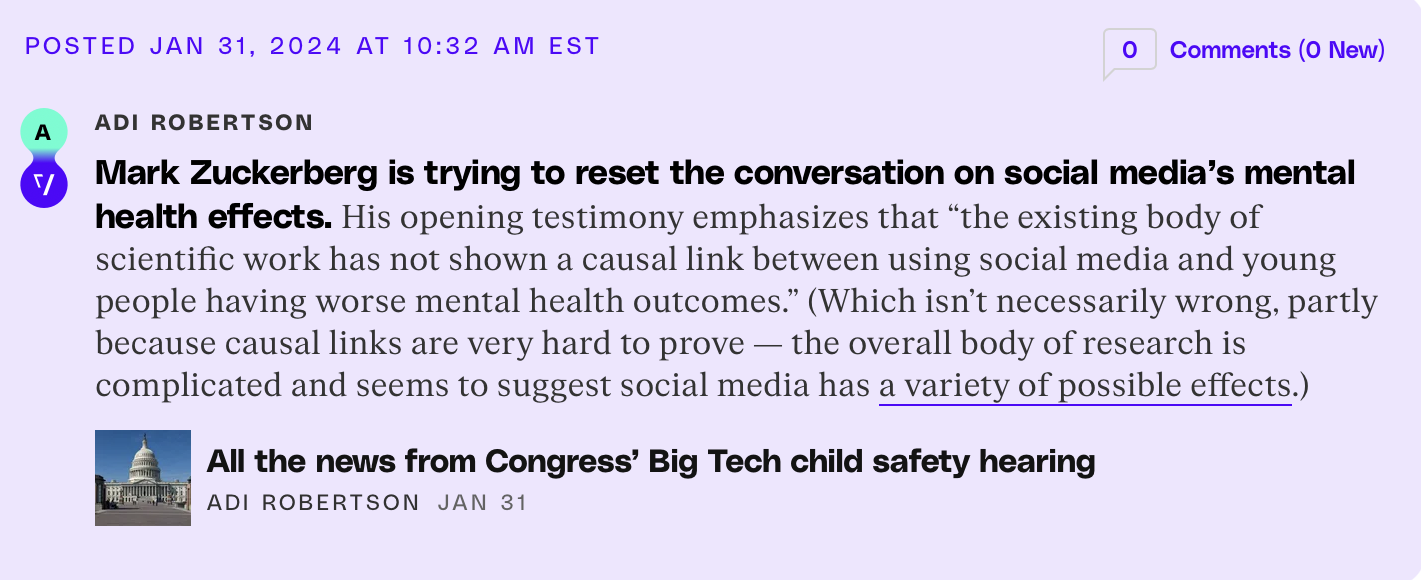
\includegraphics[scale=0.35]{./lecture_includes/facebook_quote}
\end{center}
\end{frame}



\begin{frame}{Mental health and Social Media}

\begin{itemize}
\item Unclear what he means; he may mean there is no experimental evidence
\item Very difficult to imagine a convincing randomized experiment passing IRB now at this point
\item Quasi-experimental evidence can step in to answer important questions like this
\item Braghieri, Levy and Makarin (2022), ``Social Media and Mental Health'', \emph{American Economic Review}, 112(11): 3660-3693


\end{itemize}

\end{frame}

\begin{frame}{Overview of design and data}

\begin{itemize}
\item Authors take advantage of a clever quirk in Facebook (then ``theFacebook'') targeted different universities from 2004 to 2006
\item They found an online data source that allowed them to pin point precisely when a university was ``treated'' with theFacebook
\item They then linked that data with a longrunning health survey of college students (both before and after) in a very clever way
\item Estimated the effect of a new social media platform's presence at a university on student revealed mental health problems

\end{itemize}

\end{frame}


\begin{frame}{Evidence I like to see}

\begin{enumerate}

\item \textbf{Bite}: \textcolor{red}{Nothing}. They cannot really show much here.  No data on Facebook usage.  They had to rely on anecdote and Facebook as a ``first mover'', but there had been Friendster and MySpace so this does weaken the paper maybe
\item \textbf{Main Results}: Very strong evidence, mostly expressed using rich survey data and questions transformed into z-scores (standard deviations)
\item \textbf{Falsifications}: \textcolor{red}{None}. Authors do not perform falsifications. Remember Miller, Johnson and Wherry looking at Medicaid's effect on Medicare eligible population?  There isn't anything like that here.
\item \textbf{Event studies}: Extremely compelling evidence and robustness across a half dozen different models
\item \textbf{Mechanism}: \textcolor{red}{Very weak in my opinion}

\end{enumerate}

\end{frame}

\begin{frame}{DiD in Court}

\begin{itemize}

\item So in many ways the strength of the project lies in a few areas:
	\begin{enumerate}
	\item Important question -- social media and youth mental health problems is a major policy question (see Zuckerberg testifying before Congress about it)
	\item Excellent research design -- difference-in-differences
	\item Meticulous data collection
	\item Data visualization is compelling
	\end{enumerate}
\item And it publishes in the premiere journal in economics, which I think shows that the research question and high quality data combined with research design can lift a paper

\end{itemize}

\end{frame}







\begin{frame}{TWFE}

\begin{equation}
Y_{icgt} = \alpha_g + \delta_t + \beta \times Facebook_{gt} + X_i \times \gamma + X_c \times \psi + \varepsilon_{icgt}
\end{equation}

\bigskip

Authors make the decision to lead with TWFE, most likely because the new methods have not yet fully been adopted and there is delayed "literacy" around the biases of TWFE

\end{frame}


\begin{frame}{Data on Facebook}

\begin{itemize}

\item When does Facebook appear at a school?  
	\begin{itemize}
	\item Facebook only publishes a fraction of that information
	\item They came up with a workaround
	\end{itemize}
\item The Wayback Machine has been taking almost daily photographs of every website since the Internet's beginning -- including the frontpage of ``TheFacebook'', which held some surprises


\end{itemize}

\end{frame}

\begin{frame}
\begin{center}
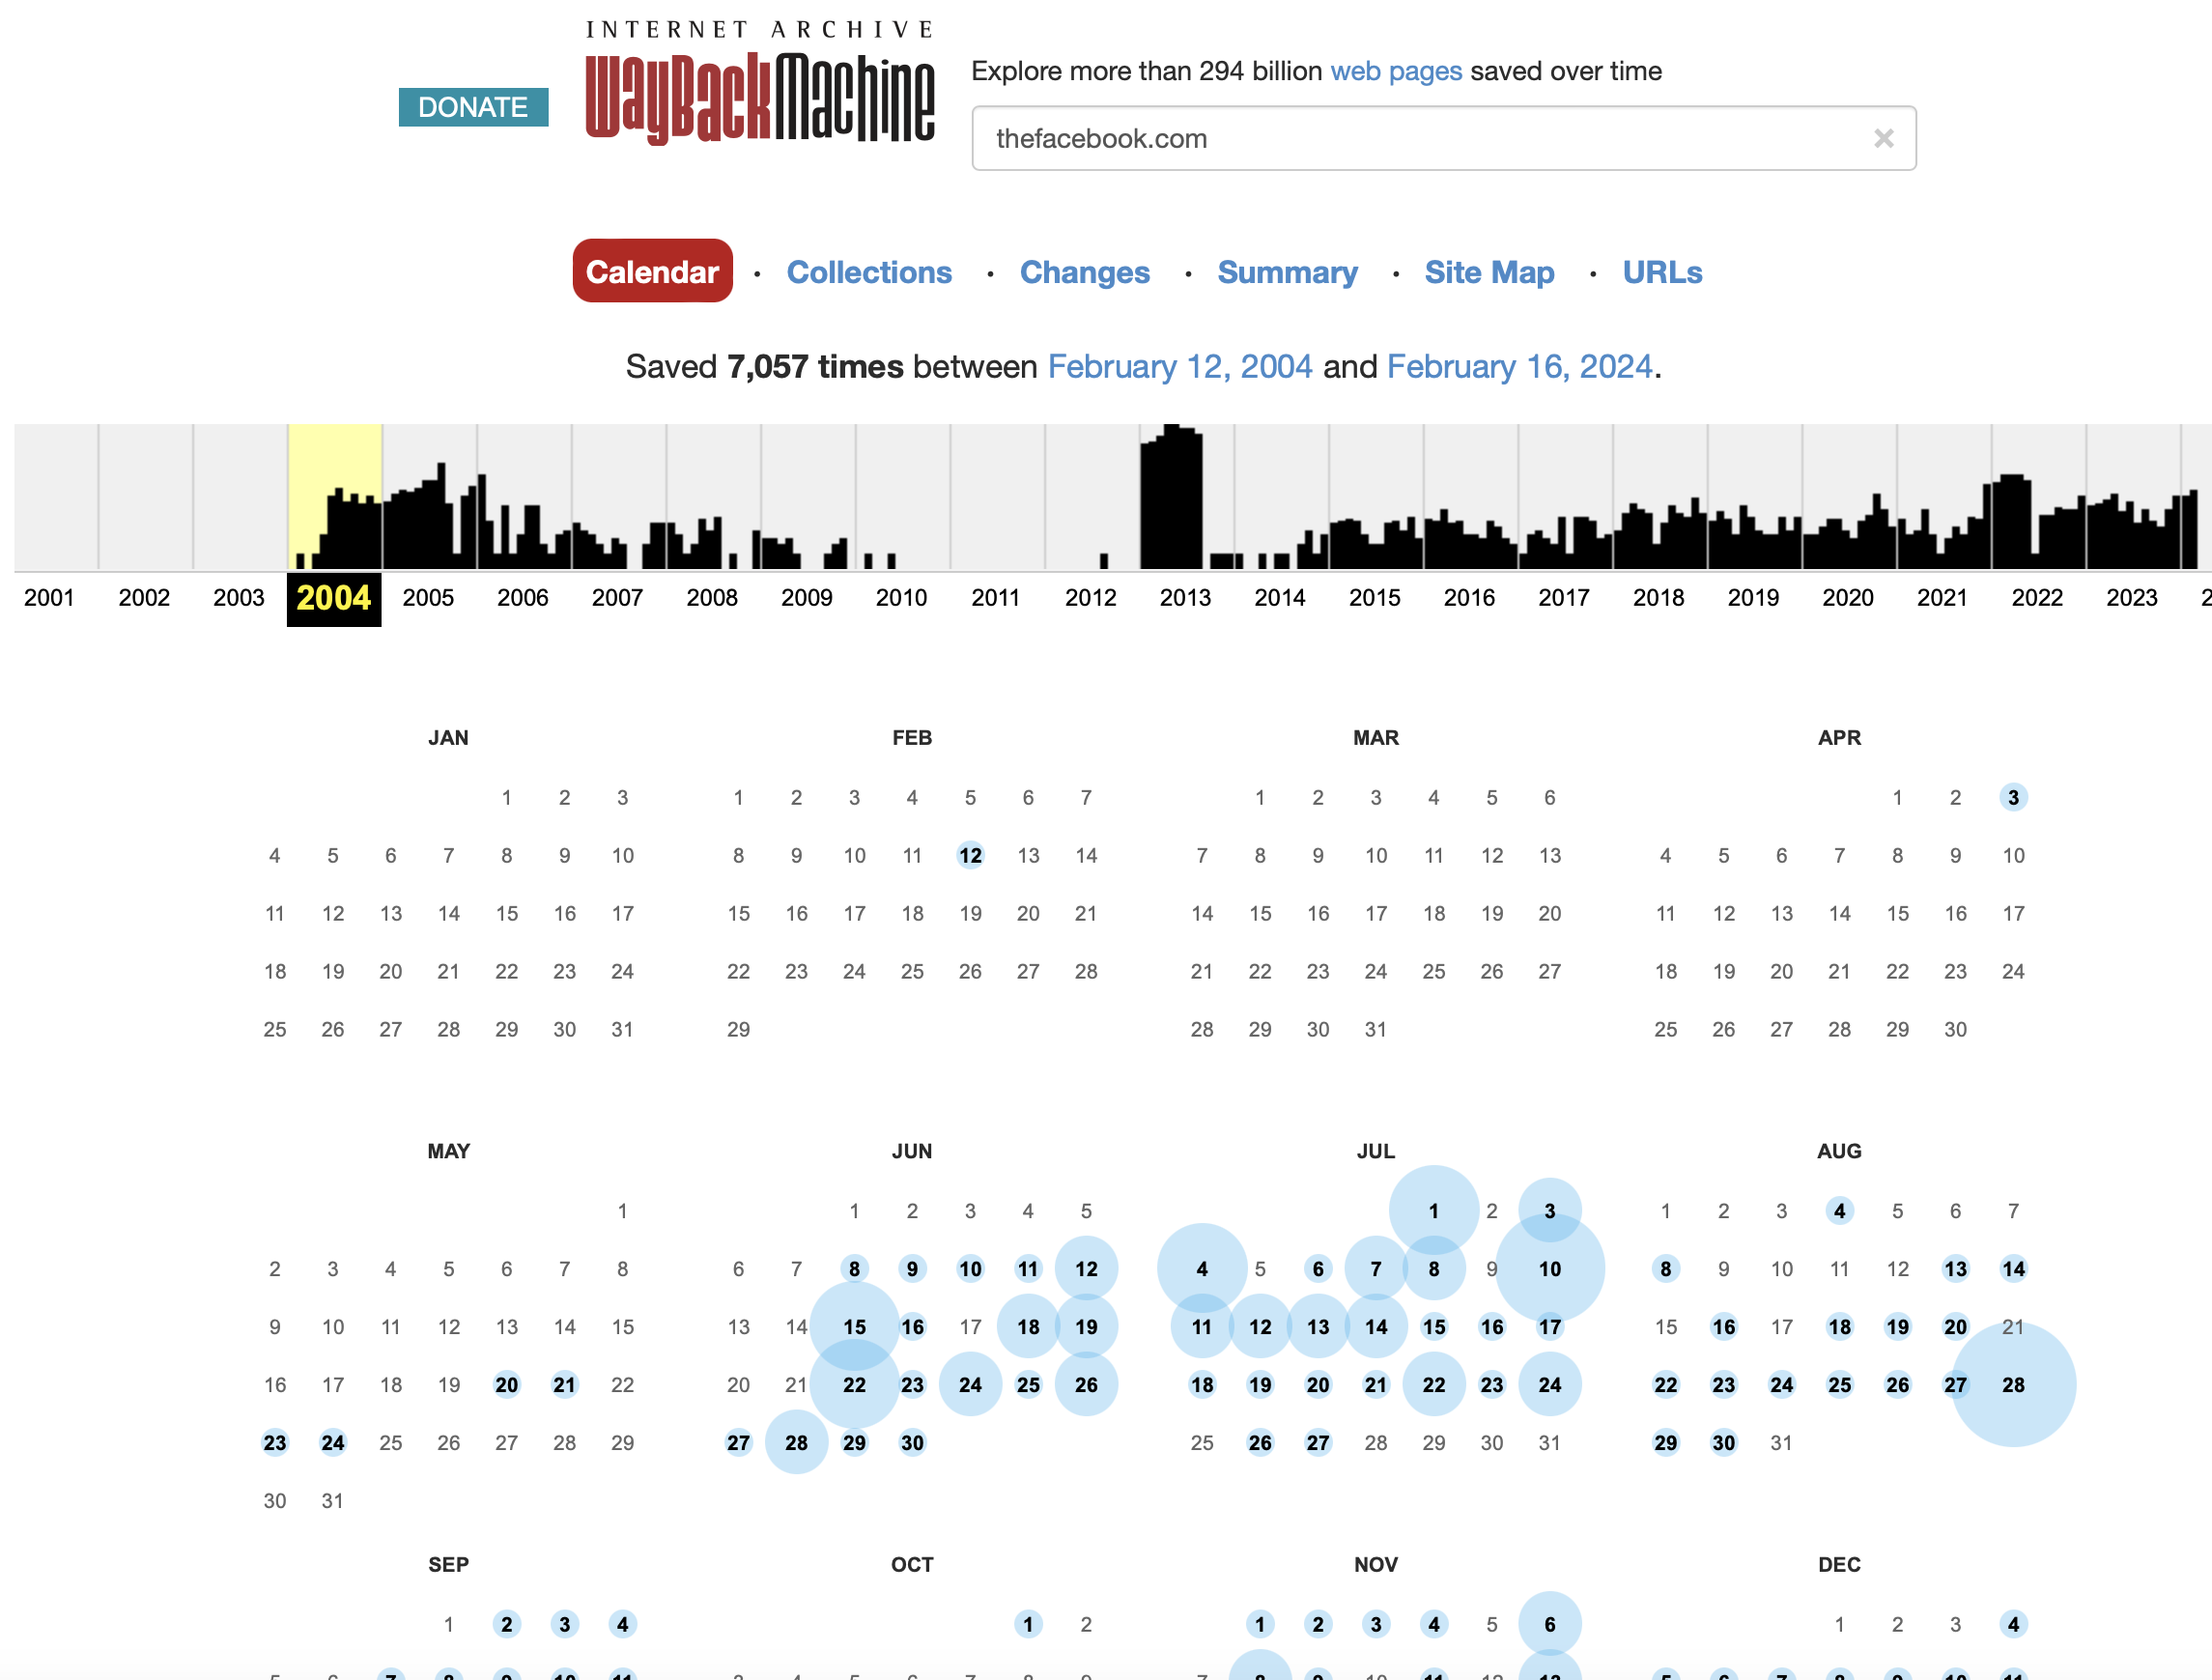
\includegraphics[scale=0.25]{./lecture_includes/wayback1}
\end{center}
\end{frame}

\begin{frame}
\begin{center}
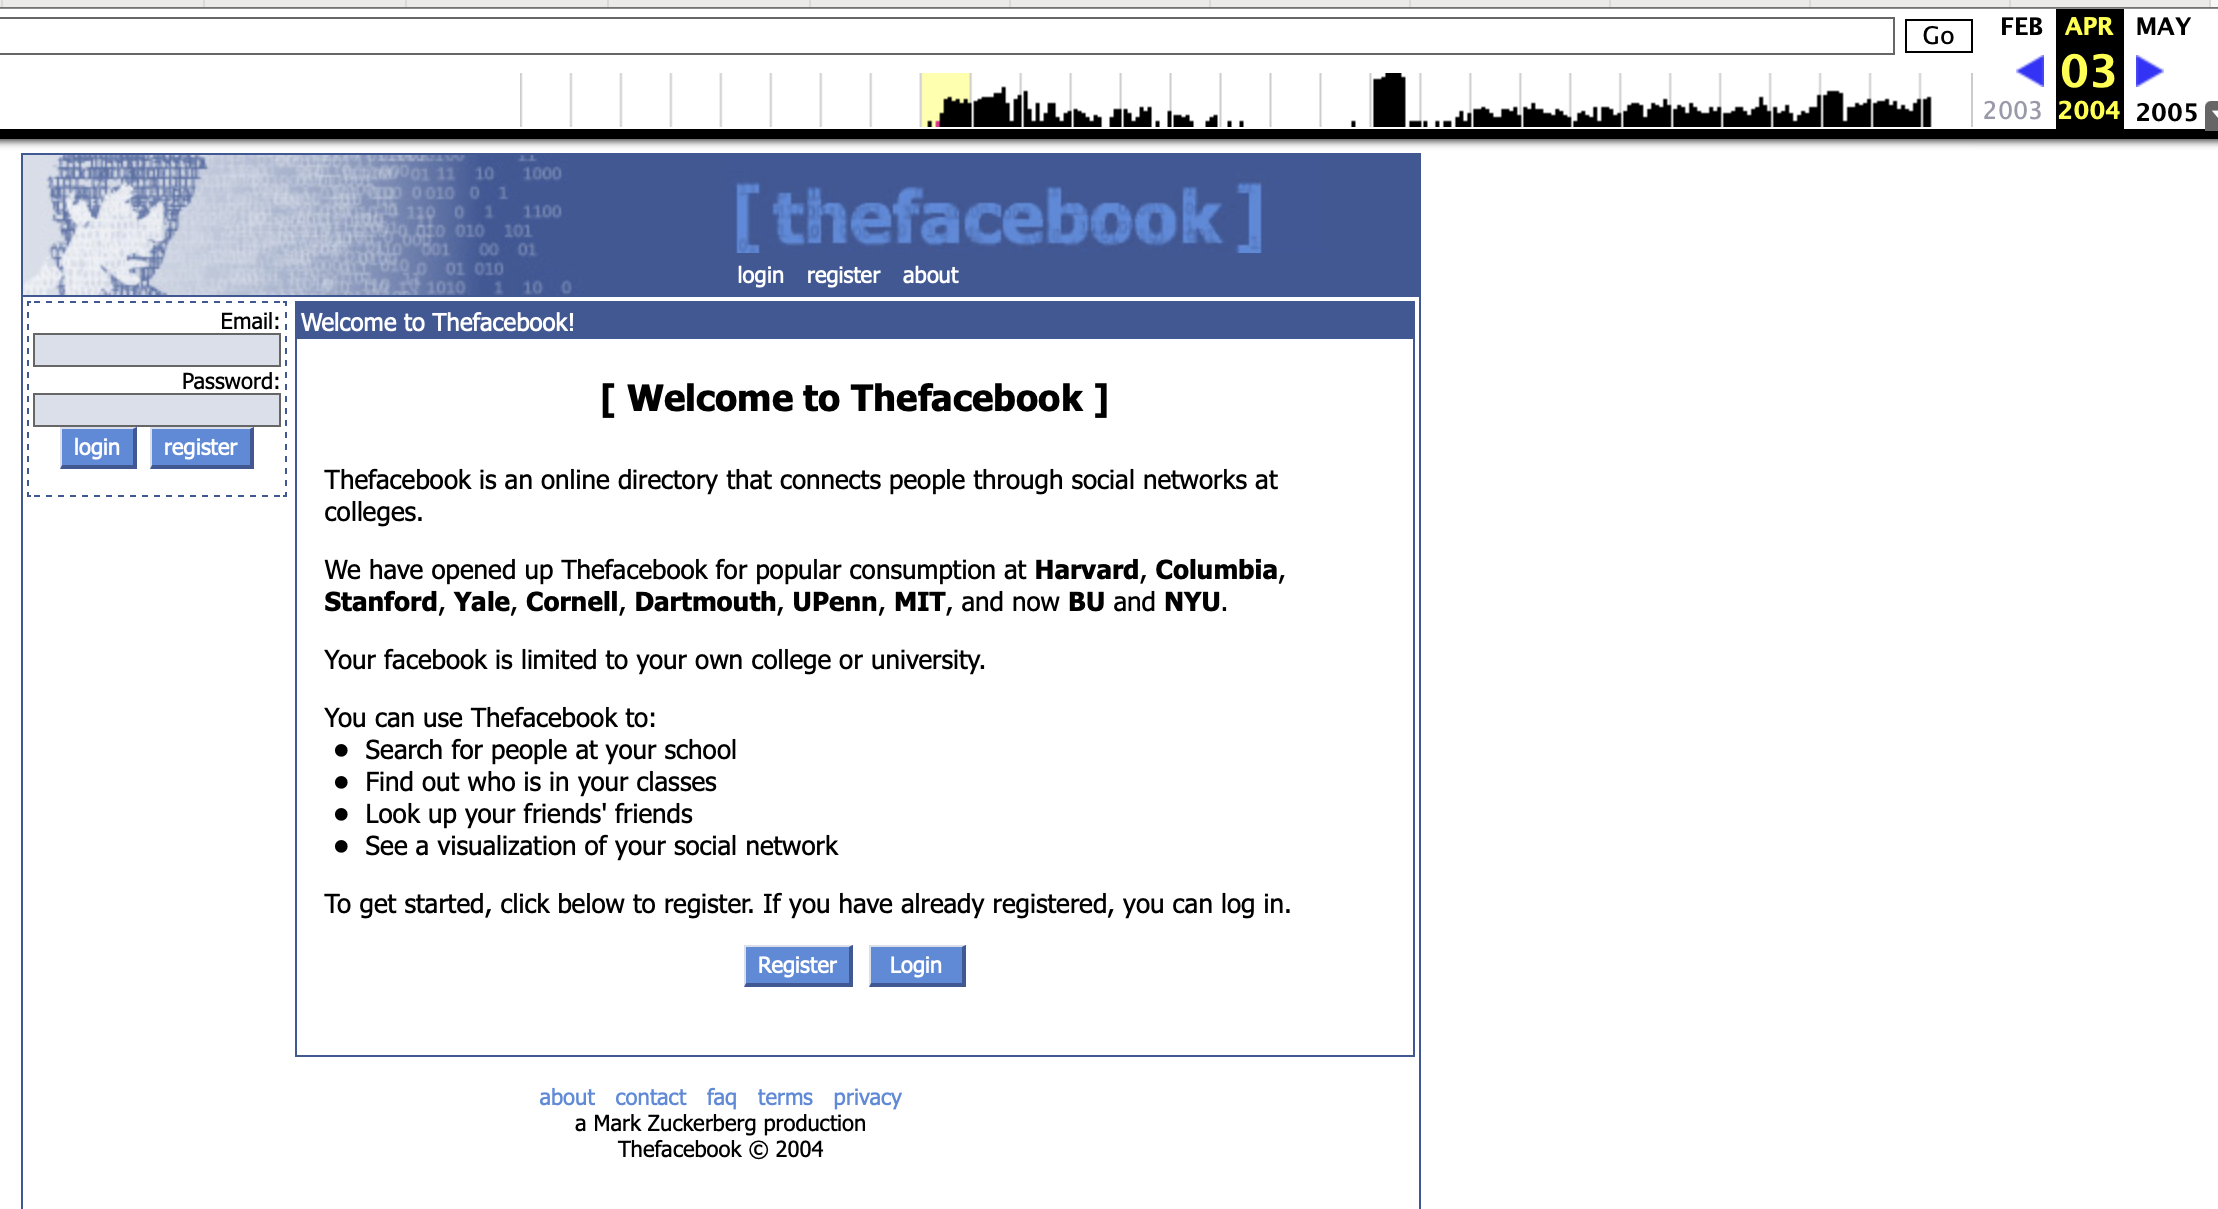
\includegraphics[scale=0.35]{./lecture_includes/wayback2}
\end{center}
\end{frame}

\begin{frame}
\begin{center}
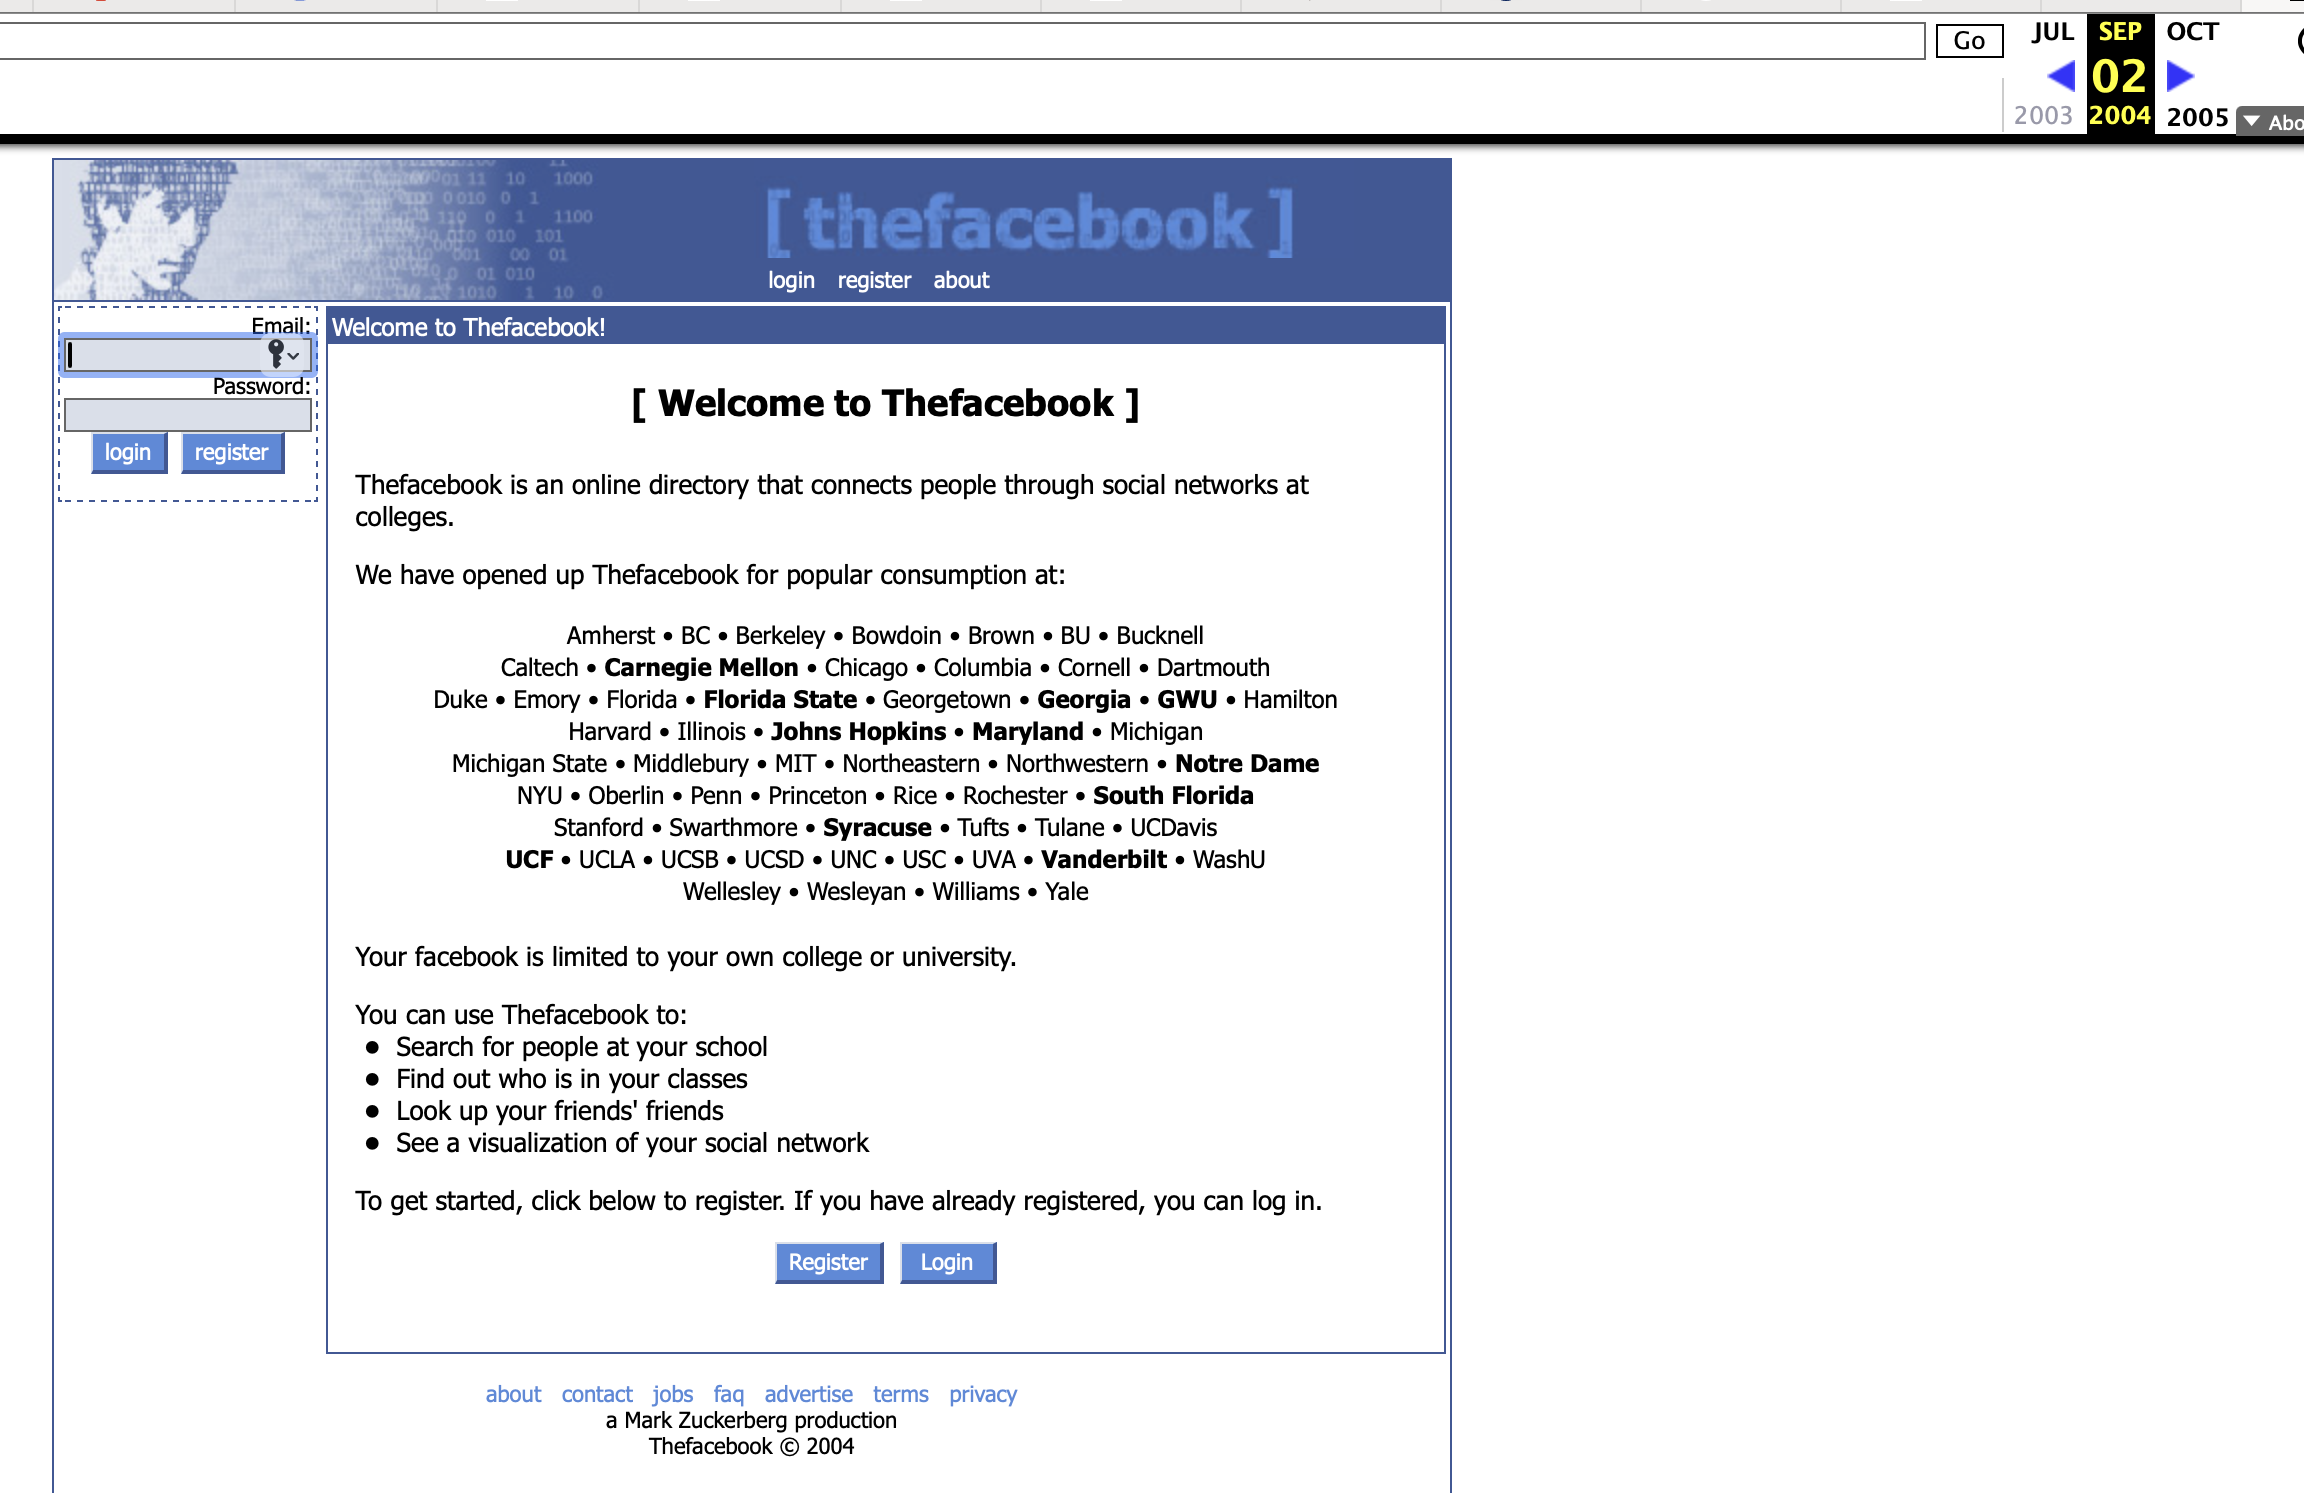
\includegraphics[scale=0.25]{./lecture_includes/wayback3}
\end{center}
\end{frame}

\begin{frame}
\begin{center}
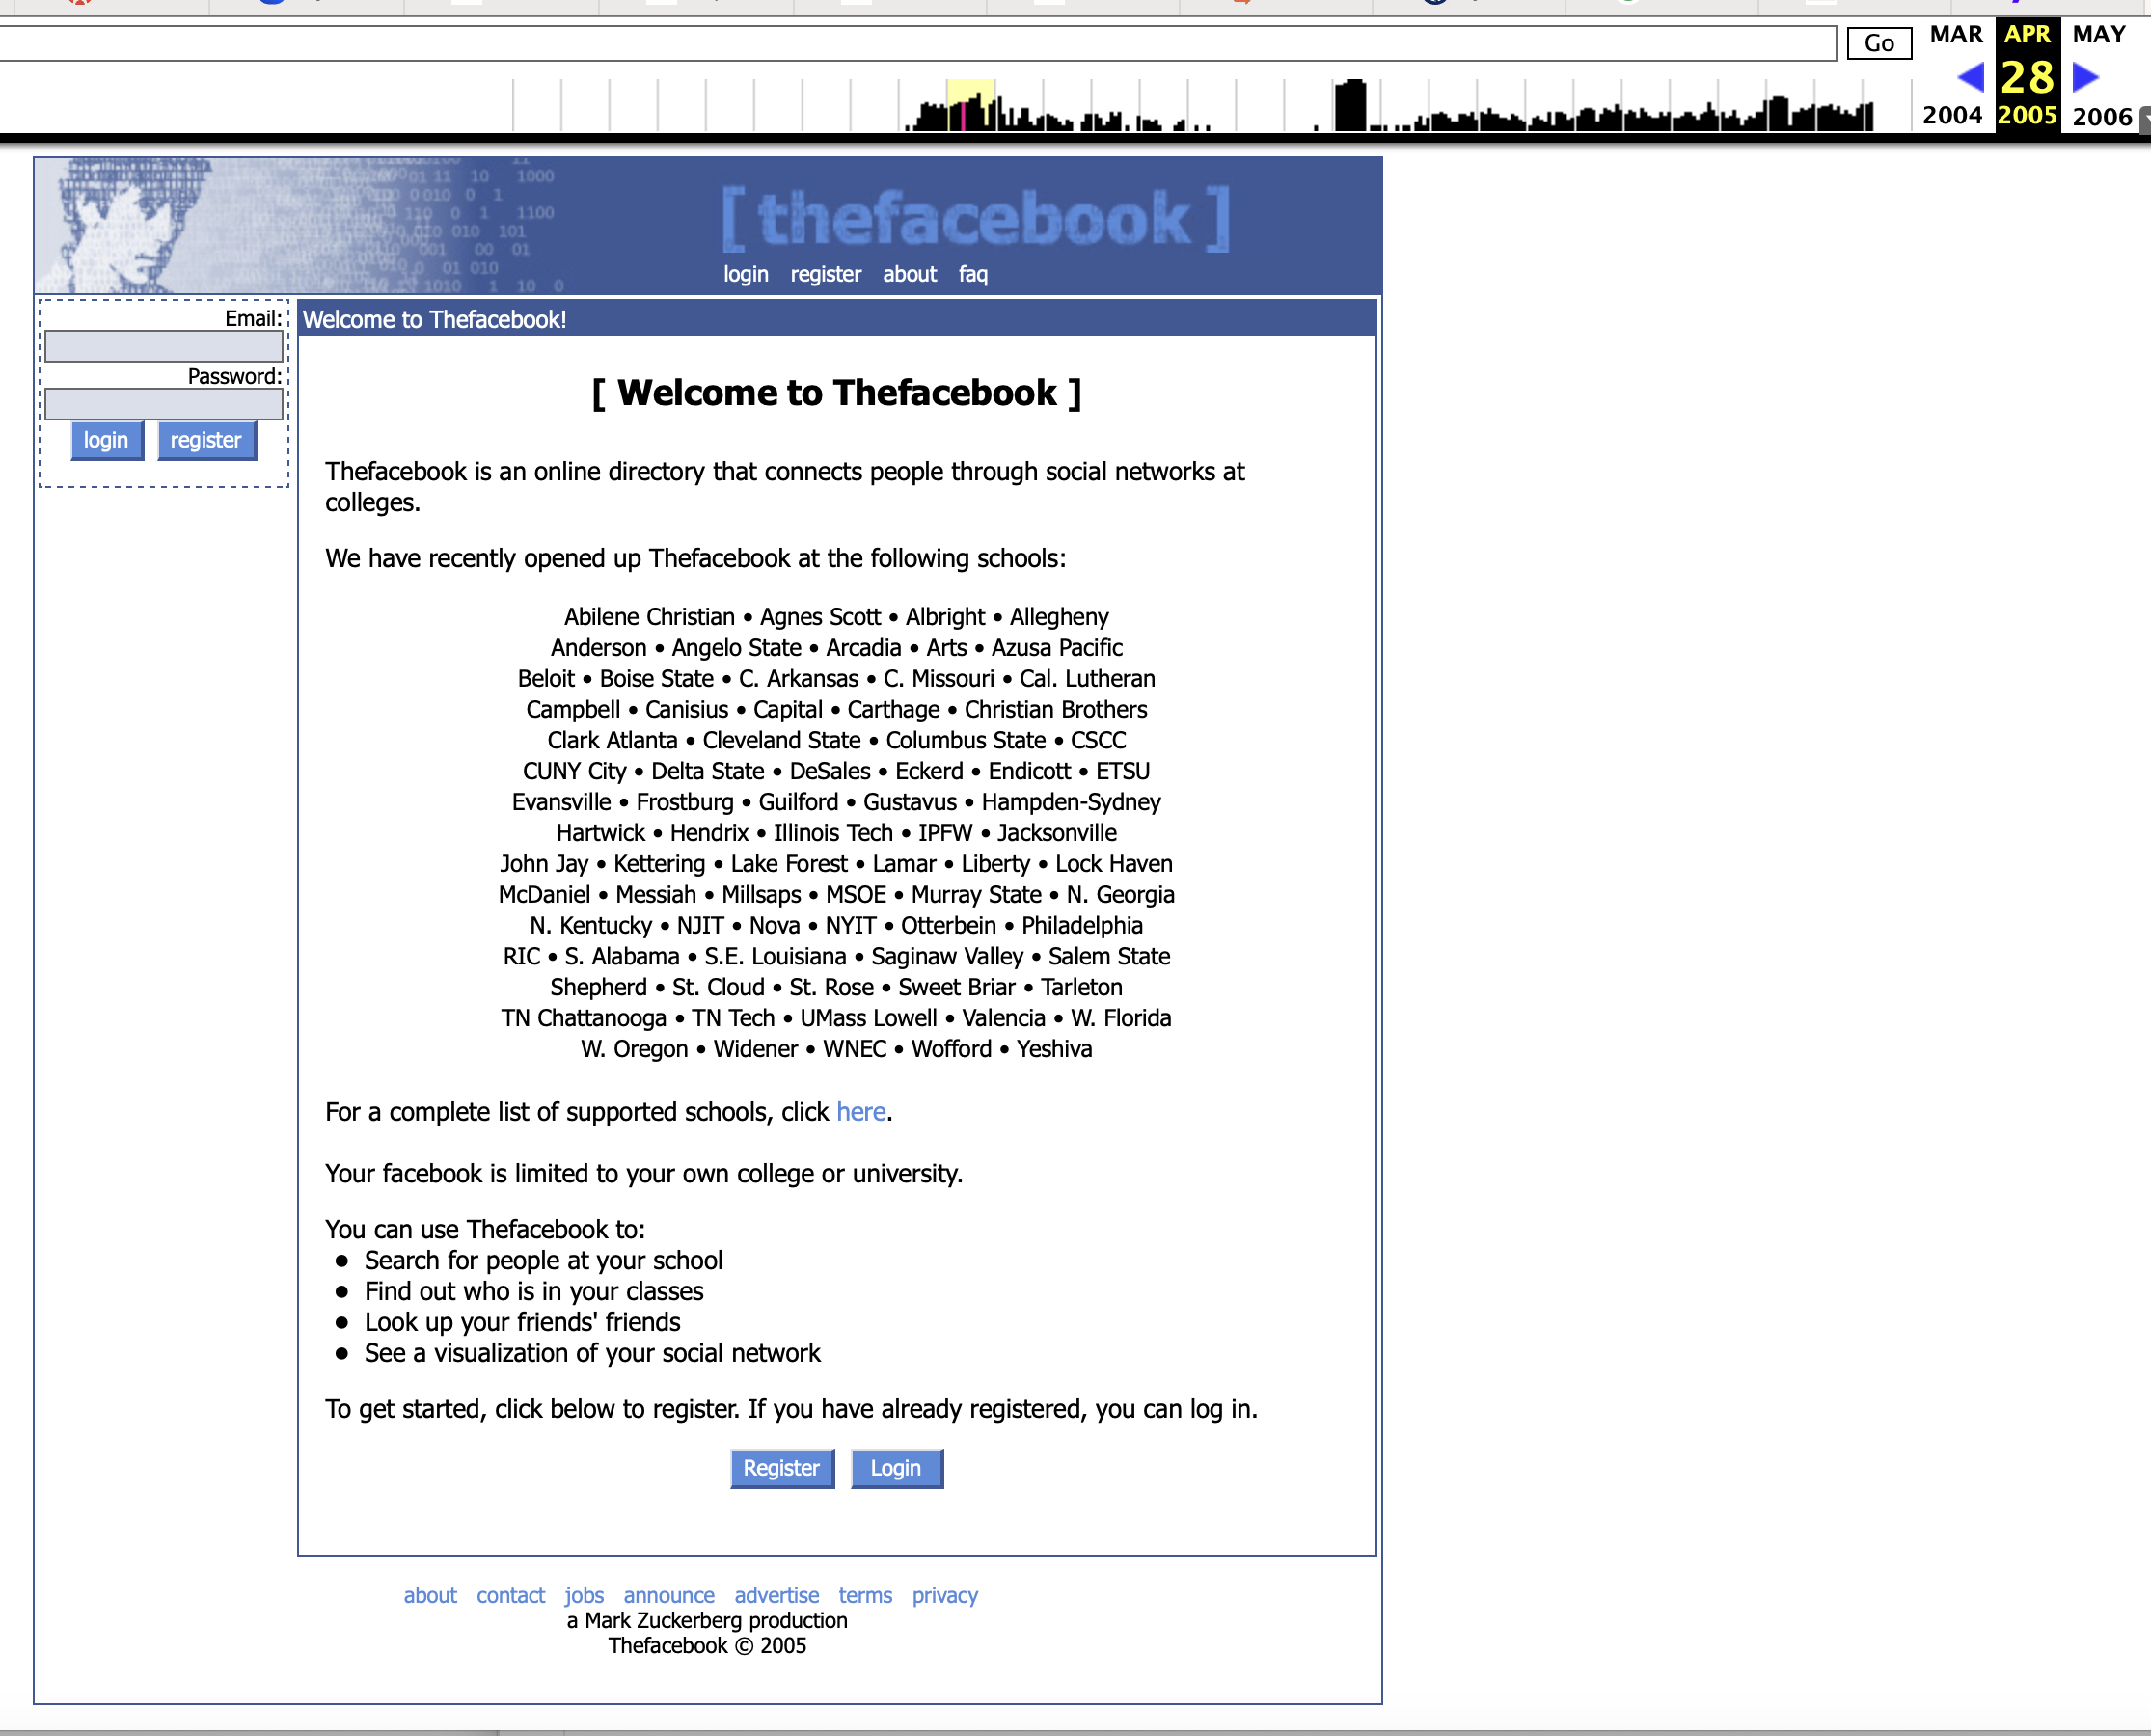
\includegraphics[scale=0.25]{./lecture_includes/wayback4}
\end{center}
\end{frame}

\begin{frame}{Timing Dates}

\begin{itemize}
\item They went through three years of daily screenshots on Wayback machine to find when a school appeared on the front page
\item The first time Penn State appears on the front page, the authors mark that as the date when the school got Facebook
\item But now they need information on mental health outcomes
\item They find it with an old long running repeated cross section survey of college students
\end{itemize}

\end{frame}

\begin{frame}{NCHA survey by ACHA}

\begin{quote}
Our second main data source consists of more than 430,000 responses to the NCHA survey, a survey administered to college students on a semi-annual basis by the American College Health Association (ACHA). The NCHA survey was developed in 1998 by a team of college health professionals with the purpose of obtaining information from college students about their mental and physical health. Specifically, the NCHA survey inquires about demographics, physical health, \textbf{mental health}, alcohol and drug use, sexual behaviors, and perceptions of these behaviors among one’s peers.
\end{quote}

\end{frame}

\begin{frame}{No evidence of bite}

\begin{quote}
The NCHA survey does not include any questions on social media use; therefore, it is not possible for us to determine whether a particular survey respondent had a Facebook account.
\end{quote}

\bigskip

This is probably the problem in any study in which your treatment is more or less the first of its kind -- most likely the standard surveys have not yet incorporated the questions into their surveys

\end{frame}

\begin{frame}{Linking Facebook data with NCHA data}

\begin{quote}
In order to protect the privacy of the institutions that participate in the NCHA survey while still allowing us to carry out the analysis, the ACHA kindly agreed to provide us with a customized dataset that includes a variable indicating the semester in which Facebook was rolled out at each college. Specifically, the ACHA adopted the following procedure: (i) merge our dataset containing the Facebook introduction dates to the NCHA dataset; (ii) add a variable listing the semester in which Facebook was rolled out at each college;15 (iii) strip away any information that could allow us to identify colleges (including the specific date in which Facebook was introduced at each college).
\end{quote}

\end{frame}

\begin{frame}{Basic facts about early and late adopters}

\begin{itemize}
\item Colleges in earlier Facebook expansion groups are more selective in terms of test scores, larger, more likely to be on the East Coast, and have more residential undergraduate programs than colleges in later Facebook expansion groups. 

\item Colleges in earlier Facebook expansion groups enroll students from relatively more advantaged economic backgrounds. 

\item Students in colleges that received Facebook relatively earlier have worse baseline mental health outcomes than students attending colleges in later Facebook expansion groups. 

%The baseline differences across Facebook expansion groups may lead one to wonder about the plausibility of the parallel trends assumption in this setting; we address concerns related to parallel trends in Section III.

\end{itemize}

\end{frame}

\begin{frame}{Measurement}

\begin{itemize}
\item The survey data is very rich with a lot of questions about mental health with different scales
\item They create their own combinations of these questions into aggregate indices -- ``index of poor mental health'' where higher numbers mean worse mental health
\item Each outcome survey question is normalized into what is called a ``z-score'' which is interpreted as a fraction of a standard deviation
\item Estimates are ATT parameters -- average effect of Facebook on students at schools that got Facebook
\end{itemize}

\end{frame}


\begin{frame}
\begin{center}
\includegraphics[scale=0.35]{./lecture_includes/facebook_1}
\end{center}
\end{frame}

\begin{frame}
\begin{center}
\includegraphics[scale=0.35]{./lecture_includes/facebook_2}
\end{center}
\end{frame}

\begin{frame}
\begin{center}
\includegraphics[scale=0.35]{./lecture_includes/facebook_3}
\end{center}
\end{frame}

\begin{frame}
\begin{center}
\includegraphics[scale=0.35]{./lecture_includes/facebook_4}
\end{center}
\end{frame}

\begin{frame}
\begin{center}
\includegraphics[scale=0.35]{./lecture_includes/facebook_5}
\end{center}
\end{frame}

\begin{frame}
\begin{center}
\includegraphics[scale=0.35]{./lecture_includes/facebook_6}
\end{center}
\end{frame}

\begin{frame}
\begin{center}
\includegraphics[scale=0.35]{./lecture_includes/facebook_7}
\end{center}
\end{frame}

\begin{frame}{Questions and Comments}

\begin{itemize}
\item Had this study been done five years ago, the conclusion of the event study would've been much different, and the paper may not have been as easily published let alone in the AER
\item No doubt more work is needed, but you can see here the power of the well designed DID and its acceptance at answering causal questions for major policy problems 
\item While the RCT would definitively answer nearly anything we can imagine, it is oftentimes not practical or even sometimes ethical raising the marginal value of the quasi-experimental design
\item But these are not straightforward either and can be easily done badly even in good faith

\end{itemize}

\end{frame}





\begin{frame}{My Preferred Ladder of Evidence}

\begin{enumerate}
\item Main results are your claim, not your evidence
\item Show bite -- first order effects are essential evidence
\item Event study graphs are one of your strongest pieces of evidence
\item Falsifications -- If you can find falsifications, use them
\item Mechanisms -- can you find any explanation?
\end{enumerate}

\end{frame}

\begin{frame}{Synthetic control}

\begin{itemize}

\item But what if parallel trends really isn't realistic -- what then?
\item Then you may need to create your own control group that follows the same approximately trajectory as your treatment group pre-treatment
\item A method by Abadie and Gardazebal (2003) and follow up papers worked out a method for this called synthetic control

\end{itemize}

\end{frame}






\end{document}


